%% ----------------------------------------------------------------
%% Thesis.tex -- MAIN FILE (the one that you compile with LaTeX)
%% ---------------------------------------------------------------- 

% Set up the document
\documentclass[a4paper, 11pt, oneside]{Thesis}  % Use the "Thesis" style, based on the ECS Thesis style by Steve Gunn
\graphicspath{{Figures/}}  % Location of the graphics files (set up for graphics to be in PDF format)

%Rearrange the CMAP
%\usepackage[resetfonts]{cmap}

%Add XMP data need to include file call metadata.xmp
\usepackage{xmpincl}
\includexmp{metadata}


\usepackage[usenames,dvipsnames]{xcolor}

\usepackage{pdfpages}



% Include any extra LaTeX packages required
\usepackage[square, numbers, comma, sort&compress]{natbib}  % Use the "Natbib" style for the references in the Bibliography
\usepackage{verbatim}  % Needed for the "comment" environment to make LaTeX comments
\usepackage{vector}  % Allows "\bvec{}" and "\buvec{}" for "blackboard" style bold vectors in maths

\hypersetup{allcolors=Blue, colorlinks=true}  % Colours hyperlinks in blue, but this can be distracting if there are many links.

%Tabulary for Scrivener MMD compatibility
\usepackage{tabulary}

%dcolumn for stargazer - delete if not required
\usepackage{dcolumn}

% Change default Bibliography name to References
\renewcommand{\bibname}{References}

%\usepackage{subfig}
%\captionsetup{belowskip=4pt,aboveskip=4pt}

\usepackage{etoolbox}% http://ctan.org/pkg/etoolbox
\AtBeginEnvironment{figure}{\addvspace{5mm}}\AtEndEnvironment{figure}{\addvspace{5mm}}
\AtBeginEnvironment{table}{\addvspace{5mm}}\AtEndEnvironment{figure}{\addvspace{5mm}}
%\AtBeginEnvironment{figure}{\addvspace{5mm}}


%% ----------------------------------------------------------------
\begin{document}
\frontmatter	  % Begin Roman style (i, ii, iii, iv...) page numbering
% Set up the Title Page
\title  {Recognition of STEMI by Paramedics and the Effect of Computer inTerpretation (RESPECT) pilot study}
\addresses  {\groupname\\\deptname\\\univname}  % Do not change this here, instead these must be set in the "Thesis.cls" file, please look through it instead
\authors  {\texorpdfstring
            {\href{http://uk.linkedin.com/pub/richard-pilbery/6b/828/413}{Richard Pilbery}}
            {Richard Pilbery}
            }

\date       {\today}
\subject    {A dissertation submitted in partial fulfilment for the degree of Masters of Clinical Research}
\keywords   {Paramedic, 12-lead ECG, STEMI, clinical research, decision making, myocardial infarction, heart attack, Randomised controlled trial, crossover, pilot}

\maketitle
%% ----------------------------------------------------------------

\setstretch{1.3}  % It is better to have smaller font and larger line spacing than the other way round

% Define the page headers using the FancyHdr package and set up for one-sided printing
\fancyhead{}  % Clears all page headers and footers
\rhead{\thepage}  % Sets the right side header to show the page number
\lhead{}  % Clears the left side page header

\pagestyle{fancy}  % Finally, use the "fancy" page style to implement the FancyHdr headers

\setcounter{page}{2}
% The "Funny Quote Page"
\pagestyle{empty}  % No headers or footers for the following pages

\null\vfill
% Now comes the "Funny Quote", written in italics
\textit{As with many interventions intended to prevent ill health, the effectiveness of parachutes has not been subjected to rigorous evaluation by using randomised controlled trials. Advocates of evidence based medicine have criticised the adoption of interventions evaluated by using only observational data.  We think that everyone might benefit if the most radical protagonists of evidence based medicine organised and participated in a double blind, randomised, placebo controlled, crossover trial of the parachute.}

\begin{flushright}
CS Smith and JP Pell \cite{smith_parachute_2003}
\end{flushright}

\vfill\vfill\vfill\vfill\vfill\vfill\null
\clearpage  % Funny Quote page ended, start a new page
%% ----------------------------------------------------------------

% The Abstract Page
\addtotoc{Abstract}  % Add the "Abstract" page entry to the Contents
\abstract{
\addtocontents{toc}{\vspace{1em}}  % Add a gap in the Contents, for aesthetics

\textbf{Background}
Timely diagnosis and appropriate management of patients with ST-segment elevation myocardial infarction (STEMI) depends on accurate interpretation of the 12-lead ECG by paramedics. Computer interpretation messages on ECGs are often provided, but the effect they exert on paramedics' decision making is not known. The pilot study objective is to assess the feasibility of conducting a trial using an online assessment tool, to determine the effect of computer interpretation messages on paramedics' diagnosis of STEMI from a 12-lead ECG.

\textbf{Methods}
The RESPECT pilot study is a randomised cross-over trial utilising a bespoke, web-based assessment tool. Participants were randomly allocated 12 of 48 ECGs, with an equal mix of correct and incorrect computer interpretation messages, and STEMI and STEMI-mimics. 

\textbf{Results}
254 Health and Care Professions Council (HCPC) registered paramedics in the UK consented into the study, 205 completing the first phase and 156 completing phase two; an attrition rate of 24\%. The ICC for participants was 0.05 and for ECGs, 0.41. Overall, participant accuracy was 80\% when the computer message was visible and 79\% when hidden. In the subset of correct computer interpretations, accuracy was 84\% (message hidden) and 87\% (message visible). The subset of incorrect computer interpretations resulted in an accuracy of 77\% (message hidden) and 71\% (message visible). Overall, the unadjusted odds ratio (OR) of a correct interpretation with a computer message was 0.94 (95\%CI 0.77--1.10, p=0.44) and adjusted OR, 0.92 (95\%CI 0.77--1.10, p=0.38). For the subset of correct computer interpretation, the unadjusted OR was 1.31 (95\%CI 1.01--1.71, p=0.04) and adjusted OR, 1.42 (95\%CI 1.06--1.89, p=0.02). Incorrect computer interpretations had an unadjusted OR of 0.76 (95\%CI 0.61--0.93, p=0.01) and adjusted OR, 0.70 (95\%CI 0.56--0.88, p=0.00).

\textbf{Conclusion}
Data from the pilot study suggests the main study is feasible, assuming the sample size calculation for the main study is not prohibitively large.


}

\clearpage  % Abstract ended, start a new page
%% ----------------------------------------------------------------

\setstretch{1.3}  % Reset the line-spacing to 1.3 for body text (if it has changed)

% The Acknowledgements page, for thanking everyone
\acknowledgements{
\addtocontents{toc}{\vspace{1em}}  % Add a gap in the Contents, for aesthetics

First and foremost I would like to thank my supervisor, Steve Goodacre, for his enthu-siasm and advice, and for re-reading endless drafts of various chapters of this dissertation.  In addition, he and Francis Morris assumed the role of `senior doctors with specialist knowledge of ECGs', providing the reference standard for the ECGs used in the study.  Indeed, this study would not have got very far without the ECGs used in the assessment tool and thanks need to go to Tom Bouthillet and Chris Watford for providing a number of these.

Whoever advised me to consult a statistician during the planning of a study also deserves much praise, although I cannot recollect where I first heard those words.  A seemingly simple study that recorded binary responses to a question about the presence of STEMI, turned out to have a rather complex analysis, involving clustering and cross-classified modelling, and I am indebted to Dawn Tere for assisting me through the minefield of binary logistic regression with random effects.  

Friends and colleagues also deserve thanks, not least those who gave up their time to undertake the ECG `quiz' and generate the data I needed, as does the College of Paramedics Research and Development Committee, who were very supportive in advertising the study.

}
\clearpage  % End of the Acknowledgements
%% ----------------------------------------------------------------

\pagestyle{fancy}  %The page style headers have been "empty" all this time, now use the "fancy" headers as defined before to bring them back


%% ----------------------------------------------------------------
\lhead{\emph{Contents}}  % Set the left side page header to "Contents"
\tableofcontents  % Write out the Table of Contents

%% ----------------------------------------------------------------
\afterpage{\blankpage}

%% ----------------------------------------------------------------
\lhead{\emph{List of Figures}}  % Set the left side page header to "List if Figures"
\listoffigures  % Write out the List of Figures

%% ----------------------------------------------------------------
\lhead{\emph{List of Tables}}  % Set the left side page header to "List of Tables"
\listoftables  % Write out the List of Tables

%% ----------------------------------------------------------------
\setstretch{1.5}  % Set the line spacing to 1.5, this makes the following tables easier to read
\clearpage  % Start a new page
\lhead{\emph{Abbreviations}}  % Set the left side page header to "Abbreviations"
\listofsymbols{ll}  % Include a list of Abbreviations (a table of two columns)
{
\textbf{ACI-TIPI} & Acute cardiac ischaemia time-insensitive predictive instrument \\
\textbf{ACS} & Acute coronary syndrome \\
\textbf{AMI} & Acute myocardial infarction \\
\textbf{ASA} & Ambulance services association \\
\textbf{CAD} & Coronary artery disease \\
\textbf{CASP} & Critical appraisal skills programme  \\
\textbf{CCU} & Coronary care unit \\
\textbf{CINAHL} & Cumulative index to nursing and allied health literature \\
\textbf{CONSORT} & Consolidated standards of reporting trials \\
\textbf{CPD} & Continuous professional development \\
\textbf{CSE} & Common standard for quantitative electrocardiography \\
\textbf{CSV} & Comma-separated values \\
\textbf{ECG} & Electrocardiogram \\
\textbf{ED} & Emergency department \\
\textbf{EMS} & Emergency medical service \\
\textbf{ESC} & European society of cardiology \\
\textbf{GLM} & Generalised linear model \\
\textbf{HCPC} & Health and care professions council \\
\textbf{ICC} & Intra-class correlation coefficient \\
\textbf{IEC} & International electrotechnical commission \\
\textbf{IMMEDIATE} & Immediate myocardial metabolic enhancement during \\
\textbf{ } & initial assessment and treatment in emergency care \\
\textbf{IVCD} & Interventricular conduction delay \\
\textbf{JRCALC} & Joint royal colleges ambulance liaison committe \\
\textbf{LBBB} & Left bundle branch block \\
\textbf{LVH} & Left ventricular hypertrophy \\
\textbf{MEDLINE} & Medical literature analysis and retrieval system online \\
\textbf{MI} & Myocardial infarction \\
\textbf{MySQL} & My structured query language \\
\textbf{NAEMT} & National association of emergency medical technicians\\
\textbf{NHS} & National Health Service \\
\textbf{NIAP} & National infarct angioplasty project \\
\textbf{NSR} & Normal sinus rhythm \\
\textbf{OR} & Odds ratio \\
\textbf{PCP} & {Primary care paramedic} \\
\textbf{PDF} & {Portable document format} \\
\textbf{PHP} & {PHP: Hypertext Preprocessor (a recursive acronym)} \\
\textbf{PICO} & Population, intervention, comparison and outcome \\
\textbf{pPCI} & Primary percutaneous coronary intervention \\
\textbf{PRISMA} & Preferred reporting items for systematic reviews and meta-analyses \\
\textbf{PVC} & Premature ventricular contraction \\
\textbf{REC} & Research ethics committee \\
\textbf{RESPECT} & Recognition of STEMI by paramedics and the effect of \\
  & computer interpretation \\
\textbf{RVH} & Right ventricular hypertrophy \\
\textbf{SHO} & Senior house officer \\
\textbf{STEMI} & ST-segment elevation myocardial infarction \\
\textbf{TPI} & Thrombolytic predictive instrument \\
\textbf{UK} & United Kingdom \\
\textbf{URL} & Uniform resource locator \\
\textbf{YAS} & Yorkshire ambulance service \\
}

%% ----------------------------------------------------------------
% End of the pre-able, contents and lists of things
% Begin the Dedication page

\setstretch{1.5}  % Return the line spacing back to 1.3

%\pagestyle{empty}  % Page style needs to be empty for this page
%\dedicatory{For/Dedicated to/To my\ldots}

\addtocontents{toc}  % Add a gap in the Contents, for aesthetics


%% ----------------------------------------------------------------
\mainmatter	  % Begin normal, numeric (1,2,3...) page numbering
\pagestyle{fancy}  % Return the page headers back to the "fancy" style

% Include the chapters of the thesis, as separate files
% Just uncomment the lines as you write the chapters

\chapter{Introduction}
\label{introduction}

 \lhead{\emph{Introduction}} % Write in your own chapter title to set the page header 

\section{Health burden of coronary artery disease}
\label{healthburdenofcoronaryarterydisease}

Worldwide, coronary artery disease (CAD) is the most common cause of death, with around seven million people dying each year~\citep{steg_esc_2012}. In Europe, every sixth man and seventh woman will die from an acute myocardial infarction (AMI), or heart attack~\citep{widimsky_reperfusion_2009}. In developed countries, including the United Kingdom (UK), the incidence of myocardial infarction has been decreasing over the past 30 years~\citep{bilgi_interpretation_2012}, but there were still 125,245 inpatient episodes at National Health Service (NHS) facilities with a primary diagnosis of AMI in 2010\slash 11~\citep{british_heart_foundation_health_promotion_research_group_coronary_2012}. 

\section{Pathophysiology of myocardial infarction}
\label{pathophysiologyofmyocardialinfarction}

Coronary artery disease is almost always caused by atherosclerosis of the coronary arteries. This is a systemic, lipid (fat) driven immume\slash inflammatory disease of the medium and large arteries~\citep{falk_pathology_2003}. Over time (usually decades), atherosclerosis causes the formation of plaques; collections of lipids and cholesterol that accumulate in the intimal layer of
arteries, some of which attract macrophages (a type of white blood cell). The macrophages secrete protein dissolving enzymes and engulf the lipids, leaving behind a lipid-rich `necrotic core'. The interface between the plaque and the lumen of the artery is known as the fibrous cap.

Ruptured plaques are the most common cause of AMI~\citep{sakakura_pathophysiology_2013}, and typically involve a plaque with a thin fibrous cap~\citep{windecker_future_2013}. This rupture usually occurs during, or just after, a sympathetic nervous system trigger such as physical or sexual activity, anger, anxiety, work stress, temperature change or cocaine use~\citep{mittleman_physical_2011}. The exposed necrotic core is highly thrombogenic, leading to platelet aggregation and activation of the clotting cascade~\citep{curzen_what_2013}. Should the artery become completely occluded, blood proximal to the blockage will stagnate and may coagulate, extending the thrombosis along the artery and making subsequent reopening of the artery much more difficult~\citep{falk_pathology_2003}.

An occluded coronary artery will usually lead to myocardial cell death secondary to prolonged ischaemia, i.e. cause a myocardial infarction (MI). This process can begin in under 20 minutes, but complete necrosis of myocardial cells which have had their supplying coronary artery (or arteries) occluded, typically does not occur until 2--4 hours, and sometimes longer, have elapsed, depending upon the presence of collateral circulation, the pre-morbid state of the patient, the nature of the occlusion (intermittent or permanent) and the sensitivity of the myocytes to ischaemia, for example~\citep{thygesen_third_2012}. This provides an opportunity for timely salvage of the myocardium, improving heart function and reducing mortality, if blood flow can be restored~\citep{department_of_health_treatment_2008}. 

\section{The electrodcardiogram and AMI}
\label{theelectrodcardiogramandami}

The first step in the development of AMI is the onset of myocardial ischaemia, as oxygen delivery fails to meet demand. Clinically, this is typically identified from the patient history, presenting signs and symptoms, and interpretation of the 12-lead electrocardiogram (ECG). The ECG is a recording of the electrical activity generated by the cells of the heart, and is obtained by the placement of a number of electrodes around the heart, which provide different ‘views’ of this electrical activity~\citep{kligfield_recommendations_2007}. The resulting output on a screen or paper plots the voltage generated against time. Characteristic components of the ECG enable a clinician to recognise a number of medical conditions, including AMI. \autoref{ecgcomplex} shows the components of the ECG, including the ST segment and T wave, which are important in the recognition of a specific type of AMI, ST-segment elevation MI (STEMI)~\citep{thomas_garcia_12-lead_2000}. Ordinarily, the ST-segment is level with the baseline (typically measured at the level of the PR segment), as shown in the the normal 12-lead ECG in \autoref{ecgsegment}.

\begin{figure}[htbp]
\centering
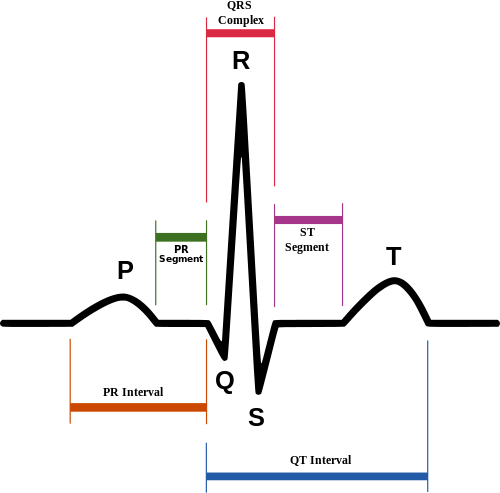
\includegraphics[keepaspectratio,width=0.6000\textwidth,height=0.75\textheight]{ECG.png}
\caption{The components of an ECG complex}
\label{ecgcomplex}
\end{figure}



\begin{figure}[htbp]
\centering
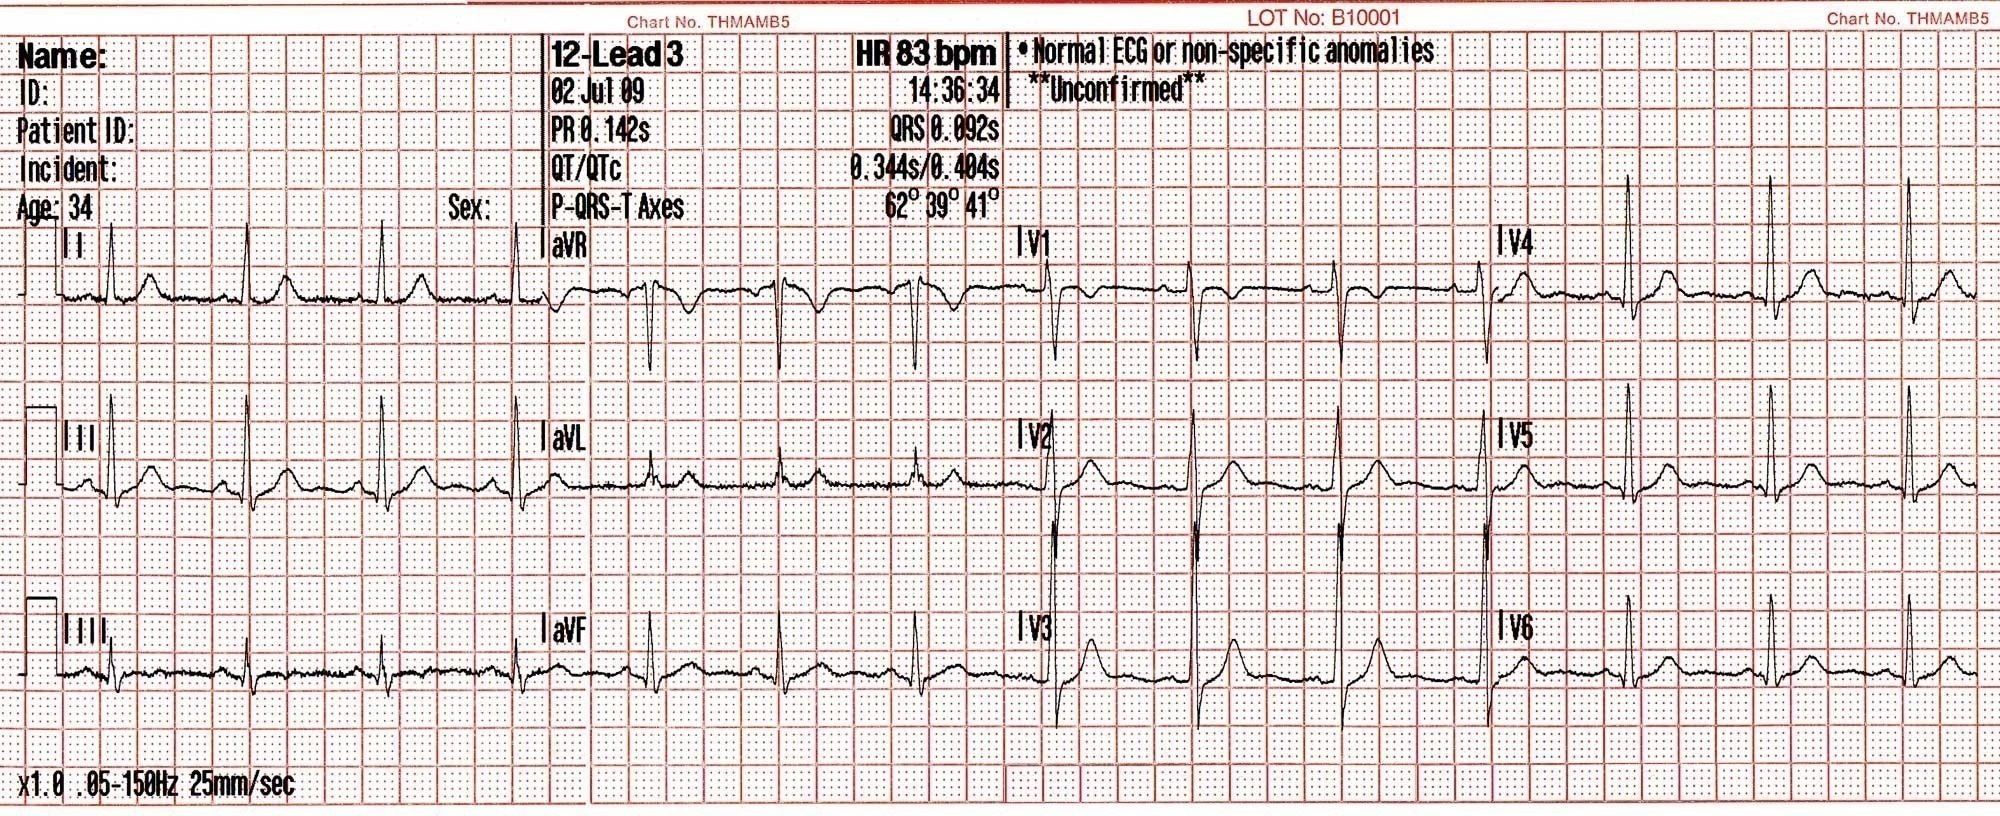
\includegraphics[keepaspectratio,width=0.9900\textwidth,height=0.75\textheight]{my-ecg-anon.jpg}
\caption{A normal 12-lead ECG}
\label{ecgsegment}
\end{figure}




During a period of myocardial ischaemia, myocardial injury often produces a characteristic rise in the ST-segment from the baseline. Criteria vary, but typically if the ST-segment rises 2mm or more in two or more leads looking at the same area of the heart, then the patient is said to be having a STEMI, even if myocardial necrosis has not yet occurred~\citep{association_of_ambulance_chief_executives_uk_2013}. \autoref{ecgstemi} shows an example of this ST-segment rise and the computer interpretation message, which is printed at the top of the 12-lead ECG.

\begin{figure}[htbp]
\centering
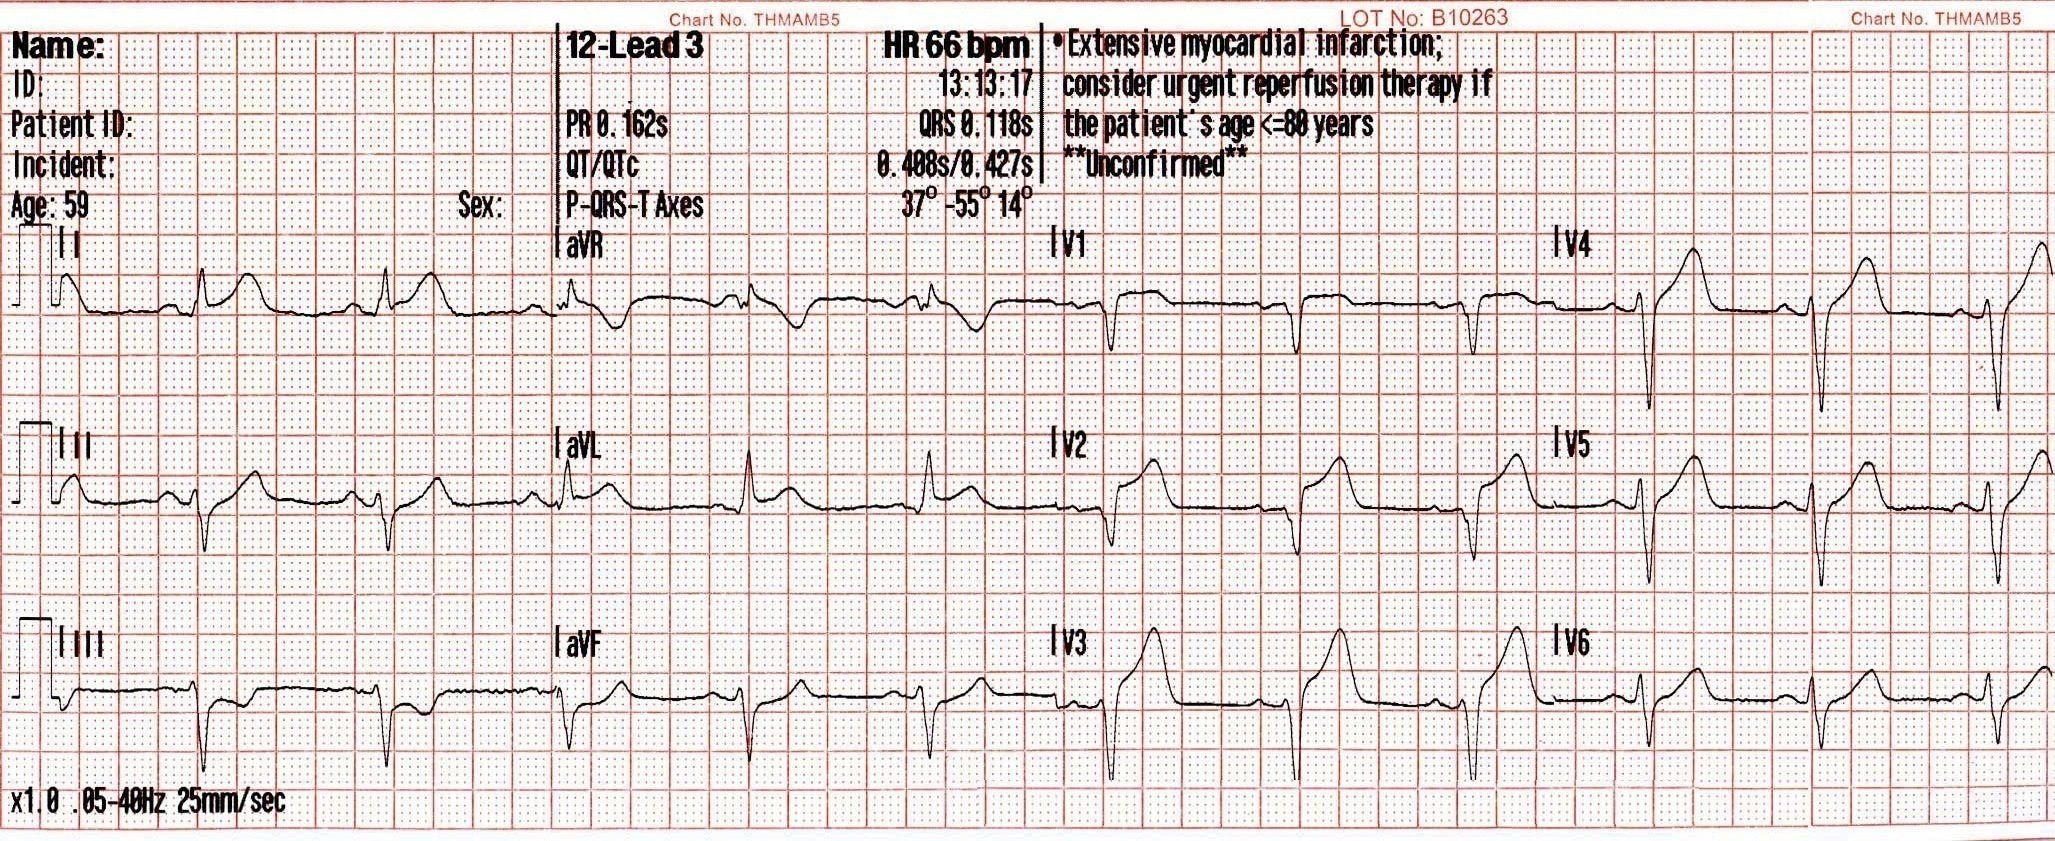
\includegraphics[keepaspectratio,width=0.9900\textwidth,height=0.75\textheight]{Sample-MI.jpg}
\caption{A 12-lead ECG with ST-segment elevation}
\label{ecgstemi}
\end{figure}



\section{Treatment of STEMI}
\label{treatmentofstemi}

Clinical trials have demonstrated a clear link between patient outcome and time to reperfusion in STEMI~\citep{department_of_health_treatment_2008}, which heightened interest in the prehospital recognition and treatment of STEMI. In 2001, prehospital thrombolysis was introduced, a technique previously only used in hospital, to chemically clear the blockage in the patient's coronary arteries. Initially, diagnosis was supported by the use of telemetry, whereby the ECG would be sent to the local hospital for diagnosis. Subsequent studies demonstrated that paramedics' diagnosis of STEMI was highly sensitive and specific~\citep{swor_prehospital_2006,feldman_real-time_2005}, leading some to question the need for telemetry with its associated costs and technical issues~\citep{woollard_limited_2005,keeling_safety_2003,johnston_paramedics_2006}. However, thrombolysis is associated with increased risk of bleeding, including haemorrhagic strokes, and is not always successful in clearing the affected coronary arteries. Fortunately, there is an alternative, mechanical clearance of coronary arteries with a balloon catheter and stent, collectively known as primary percutaneous coronary intervention (pPCI). In 2008, the National Infarct Angioplasty Project (NIAP) concluded that numerous international trials demonstrated reduced mortality and improved long-term outcome of pPCI compared with thrombolysis. However, this is time dependent, and delays beyond 90 minutes from when thrombolysis could have been administered, is considered to be point at which the benefit of pPCI is negated. In addition, NIAP also demonstrated that in order to achieve this, bypassing local hospitals in favour of a regional centre which had a cardiac catheter lab was the most effective (and cost-effective) method~\citep{department_of_health_treatment_2008}.

As with the early administration of thrombolysis, ambulance services now have an important role in minimising the time from a patient's call for professional help, to undergoing pPCI (the call-to-balloon time). In the UK, 95\% of STEMI patients are treated with pPCI, and 77.5\% of patients with STEMI are taken directly to the cardiac catheter labs by the ambulance service~\citep{ludman_national_2013}. The current European Society of Cardiology (ESC) guidelines for the management of patients presenting with STEMI, advocate the recording of a 12-lead ECG within 10 minutes of first medical contact, and direct transfer to a pPCI capable centre, if this is possible, within 120 minutes. If this is not possible, then the administration of thrombolysis should be achieved within 30 minutes~\citep{steg_esc_2012}. This guidance has been incorporated into the current UK ambulance service clinical guideline for the management of STEMI~\citep{association_of_ambulance_chief_executives_uk_2013}.

\section{Computer interpretation of ECGs}
\label{computerinterpretationofecgs}

Since Augustus Waller first demonstrated the measurement of electrical current produced by the human heart in 1887 (\autoref{jimmie})~\citep{waller_demonstration_1887,herring_ecg_2006}, ECG recording fidelity has improved considerably, as has the portability of the hardware required to produce the waveforms. 

\begin{figure}[htbp]
\centering
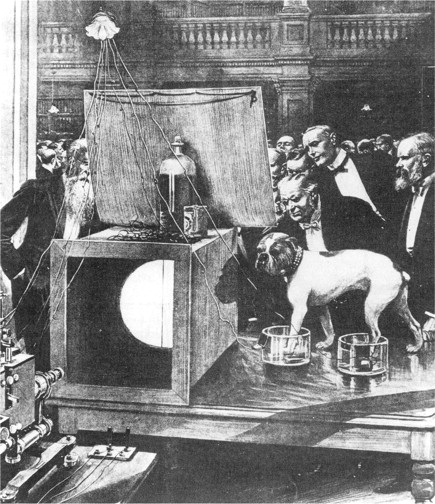
\includegraphics[keepaspectratio,width=0.5000\textwidth,height=0.75\textheight]{bulldog.jpg}
\caption{Waller demonstrating at the Royal London Society with his bulldog Jimmie}
\label{jimmie}
\end{figure}



However, recording the ECGs is just the first step, since they also require interpretation. Since skilled personnel are not universally available, computers have been seen as a possible solution. In the 1960s, computer interpretation of ECGs was introduced, although this was typically only available at larger hospitals with large, dedicated computers~\citep{willems_computer_1981}. Today, computer interpretation of ECGs is possible at the patient's side, thanks to the increased power and reduced size of computers.

In order to interpret an ECG, a computer needs to complete five steps~\citep{kligfield_recommendations_2007}:

\begin{enumerate}
\item Obtaining and filtering the signal

\item Identifying and sorting complexes in order to create an average (typically median) complex for each lead

\item Recognising the waveform and identifying the onset and offset of a single complex

\item Extracting features from complexes and measuring amplitudes and intervals

\item Utilising heuristic or statistical methods to allocate diagnoses.

\end{enumerate}

\subsection{ECG standards}
\label{ecgstandards}

In order to introduce a standard performance benchmark for the first four steps, a Common Standard for Quantitative Electrocardiography (CSE) database was created in the late 1980s (and finalised in 1990). This consists of 1220 calibrated ECGs which are provided to manufacturers to test their ECG hardware and software~\citep{willems_comparison_1991,willems_diagnostic_1991}. These ECGs were subsequently incorporated into the International Electrotechnical Commission standard IEC 60601--2--51 (superseded by IEC 60601--2--25 ed2.0 in 2011), which also includes acceptable tolerances in mean and standard deviation differences from the published measurements~\citep{international_electrotechnical_commission_medical_2011}. In addition, there are also standards relating to the messages produced by the computer interpretation algorithm. Examples of these are shown in \autoref{bethesda}~\citep{rautaharju_task_1978}.

\begin{table}[htbp]
\begin{minipage}{\linewidth}
\setlength{\tymax}{0.5\linewidth}
\centering
\small
\caption{ECG computer interpretation statements}
\label{bethesda}
\begin{tabulary}{\textwidth}{@{}CLL@{}} \toprule
\textbf{Type}&\textbf{Description}&\textbf{Example}\\
\midrule
A&Diagnosis of an anatomical lesion relating to pathophysiological state&Interior infarct\\
B&Diagnosis of electrophysiological changes&Left bundle branch block\\
C&Descriptive ECG features&Nonspecific ST abnormality\\

\bottomrule

\end{tabulary}
\end{minipage}
\end{table}


\subsection{Computer interpretation algorithms}
\label{computerinterpretationalgorithms}

Probably the most ubiquitous ECG interpretation algorithm in use by UK ambulance personnel is the General Electric (GE) Healthcare Marquette 12SL ECG analysis program~\citep{ge_healthcare_marquette_2010}. This is a heuristic algorithm, utilising experience-based, deterministic rules that incorporate measurements from the median waveform into a decision tree and boolean combinations of criteria~\citep{kligfield_recommendations_2007}.

Other algorithms adopt alternative approaches, such as statistical methods, which generate probability statements. An example is the acute cardiac ischaemia time-insensitive predictive instrument (ACI-TIPI)~\citep{selker_use_1998}. At least one algorithm in use by prehospital healthcare professionals utilises algorithms trained using artificial neural networks~\citep{eggers_artificial_2007}, although in practice, these have been found to work better if combined with more traditional, deterministic, methods rather than as a standalone method~\citep{physio_control_glasgow_2009-1}. 

\subsection{Validation of ECG algorithms}
\label{validationofecgalgorithms}

Irrespective of the method used by the ECG interpretation algorithm, there is a need for training and testing in order to validate its use more generally. This typically consists of training the algorithm on databases containing ECGs with specific, often single, pathophysiologies, for example an MI or a specific arrhythmia. Subsequent testing usually utilises much larger ECG databases, containing a wide spectrum of ECG electrophysiologies, in order to calculate sensitivity and specificity statistics. The gold standard varies, depending on what characteristic is being tested. For example, the expert opinion of a cardiologist might be appropriate for conditions such as arrhythmias whereas, in acute coronary syndromes, it is more typical for cardiac enzymes or angiography confirmation of diagnosis to be used~\citep{ge_healthcare_marquette_2008,ge_healthcare_marquette_2007}. 

\section{Recognition of STEMI by paramedics}
\label{recognitionofstemibyparamedics}

Timely diagnosis and appropriate management of patients with STEMI depends on accurate interpretation of the 12-lead ECG by paramedics. However, since only 4--6\% of chest pain calls to emergency services are actually acute coronary syndromes, this is not always straightforward~\citep{deakin_does_2006}. Thus, initial and ongoing training in the accurate acquisition and interpretation of 12-lead ECGs by paramedics, is important~\citep{ting_implementation_2008,ducas_transmit_2012}.

There is little published literature about the training provided to UK ambulance personnel in relation to ECG interpretation. The most credible is arguably a 2001 technology appraisal process document, authored by the Joint Royal College Ambulance Liaison Committee (JRCALC) and the Ambulance Services Association (ASA), which set out a suggested syllabus for a prehospital thrombolysis course~\citep{the_joint_royal_colleges_ambulance_liaison_committee_pre-hospital_2001}. This itself, was based on existing courses being run at the time by four ambulance services and included the following topic areas:

\begin{enumerate}
\item ECG acquisition

\item Components of a `normal' ECG

\item Arrhythmias

\item Coronary artery disease

\item The ECG in coronary artery disease

\item Management of MI including thrombolytics and other drugs.

\end{enumerate}

Two courses were created by pharmaceutical companies who manufactured thrombolysis drugs, namely Fast Track to Thrombolysis by Roche, and Thrombolysis Up Front by Boehringer Ingelheim. These courses were provided free of charge to UK ambulance services, and although there are no national statistics regarding the utilisation of such course material, Thrombolysis Up Front was used by every UK ambulance service at that time~\citep{watts_thrombolysis_2013}.

In the absence of telemetry, computer aided interpretation of the 12-lead ECG is an attractive option, and is available on all ECG monitors carried by UK ambulance services (although at extra cost). Depending on the study, computer interpretation alone is 58--78\% sensitive and 90--100\% specific, with false positive rates varying between 19--39\%~\citep{bhalla_prehospital_2013,clark_automated_2010,youngquist_comparison_2008}. Most studies consist of a mixture of paramedic and computer interpretation combined, either embedded in a protocol (usually requiring paramedic and computer agreement), or available for the paramedic to optionally utilise as a diagnostic tool. Sensitivities in this instance fall in the range 68--99.6\%, specificities 68--97\% and false positive rates 12--40\%~\citep{cantor_prehospital_2012,ducas_transmit_2012,ioannidis_accuracy_2001,mixon_retrospective_2012,ting_abstract_2009,young_paramedics_2011}. However, with the exception of one study, in which the computer interpretation was deliberately switched off, it is difficult to unpick what effect the computer interpretation, and the paramedic's own diagnostic skills, contribute to the figures mentioned. If it is the case that computer interpretation is adversely affecting accurate interpretation of the ECG, then it can be switched off. It may be the case, that the initial, and continuing, education of paramedics is the key. However, it is also possible that maintaining the status quo (i.e. a combination of paramedic and computer interpretation) is the best option. 

\section{Consequences of false negatives and positives}
\label{consequencesoffalsenegativesandpositives}

In contrast to early studies examining paramedics' safe administration of thrombolysis, false-positive rates for pPCI referral, have been reported to be 20--31\%~\citep{young_paramedics_2011,davis_positive_2007,rokos_appropriate_2010,swan_factors_2009}, possibly due to poor ECG recording, mis-interpretation of the ECG and\slash or the perception that pPCI is less risky than administering thrombolytics~\citep{smith_st-elevation_2001}. Inappropriate referral to pPCI centres has potential cost implications, may contribute to staff burnout, particularly for hospital staff who are called in from home out-of-hours, and result in longer patient transport times to a regional pPCI centre, rather than the local emergency department (ED), which is associated with an increased risk of mortality~\citep{nicholl_relationship_2007}.

False negatives are equally undesirable, since failure to identify and appropriately manage patients with STEMI, is more likely to result in delayed time to reperfusion, with the subsequent negative impact on mortality and morbidity~\citep{department_of_health_treatment_2008}. However, existing research has not explored this in any detail. Work on thrombolysis perhaps unsurprisingly focussed on ensuring the patients paramedics choose to thrombolyse had been selected appropriately, ignoring those who may have been inappropriately missed~\citep{khan_paramedic-led_2009,pitt_prehospital_2002,smith_paramedic_2010}. In addition, research examining the prehospital activation of cardiac catheter labs, perhaps unsurprisingly, focussed on false positive rates and the impact this would have on pPCI services. However, only recruiting participants on a pPCI pathway meant that none of the studies were able to identify patients who were missed (with the exception of the Ting study~\citep{ting_abstract_2009}, which did record patients who had been taken to the ED at the study hospital). 

\section{Research focus}
\label{researchfocus}

The Recognition of STEMI by Paramedics and the Effect of Computer inTerpretation (RESPECT) aims to answer the following research question:

\begin{quote}

Do computer interpretation messages have an effect on paramedics' diagnosis of STEMI from a 12-lead ECG?
\end{quote}
 % Introduction - 2446 words

\chapter{Literature review}
\label{literaturereview}

 \lhead{\emph{Literature Review}} % Chapter title for thesis template 

\section{Search strategy}
\label{searchstrategy}

In order to identify an appropriate set of key search terms for the literature review, a population, intervention, comparison and outcome (PICO) framework was utilised (\autoref{tablepico})~\citep{sayers_tips_2008}. A brief scoping study identified that there were likely to be few studies focussing exclusively on paramedics, so the population definition was expanded to include all healthcare professionals, on the basis that although the results may not be directly applicable, they would assist in study planning. The remaining elements of the PICO framework utilised the research question as a guide.

\begin{table}[htbp]
\begin{minipage}{\linewidth}
\setlength{\tymax}{0.5\linewidth}
\centering
\small
\caption{PICO framework for RESPECT research question}
\label{tablepico}
\begin{tabulary}{\textwidth}{@{}LL@{}} \toprule
\textbf{Framework element}&\textbf{Description}\\
\midrule
Population&Healthcare professionals who are required to interpret 12-lead ECGs and recognise STEMI.\\
Intervention&Computer assisted interpretation of a 12-lead ECG by healthcare professionals to determine the presence of STEMI.\\
Comparison&An appropriate reference standard e.g. blood cardiac enzymes, angiography, expert opinion.\\
Outcome&Diagnostic accuracy of healthcare professionals' diagnosis of STEMI\\

\bottomrule

\end{tabulary}
\end{minipage}
\end{table}


The medical literature analysis and retrieval system online (MEDLINE), cumulative index to nursing and allied health literature (CINAHL), Cochrane library and Google scholar databases were searched between the 1st of December 2012 and 31st July, 2013, with no language or publication restrictions. 

\section{Inclusion and exclusion criteria}
\label{inclusionandexclusioncriteria}

Full-text articles were obtained for systematic reviews and studies that were randomised, quasi-experimental, observational or diagnostic cohort in design. Consensus statements or guidelines, which related to the prehospital management of patients with acute coronary syndrome, were reviewed in order to identify further relevant studies, but excluded from the final analysis. For a study to be considered for the final analysis, it had to be randomised, quasi-experimental, observational or diagnostic cohort in design, and include a comparison between healthcare professionals and a reference standard, in the diagnosis of STEMI. Studies which only included process measures, such as door-to-balloon or door-to-needle times, were excluded. No geographical or service type (for example public versus private) restrictions were placed on the studies. 

\section{Assessment of quality}
\label{assessmentofquality}

To aid in the evaluation of the research studies identified by the literature search, the Critical Appraisal Skills Programme (CASP) checklist was utilised~\citep{critical_appraisal_skills_programme_appraising_2013}. This evaluates published research by asking three general questions about the study and providing additional questions under each heading, to aid critical appraisal:

\begin{enumerate}
\item Is the study valid?

\item What are the results?

\item Are the results applicable to my needs?

\end{enumerate}

\section{Data extraction}
\label{dataextraction}

Although the literature review was not systematic, the methodology used to identify and extract information from the review was informed by a prehospital systematic literature review and the Cochrane handbook of systematic reviews~\citep{jensen_comparison_2010,the_cochrane_collaboration_cochrane_2011}. 

\section{Results}
\label{results}

A total of 147 titles and abstracts were obtained using the search strategy specified. Five full-text articles and one conference abstract met the inclusion criteria (see the Preferred Reporting Items for Systematic Reviews and Meta-Analyses [PRISMA] flow diagram in \autoref{prismalit})~\citep{goodacre_computer_2001,massel_observer_2003,tsai_computer_2003,ting_abstract_2009,selker_emergency_2011,cantor_prehospital_2012}. One further article was obtained, which explained the methodology used for the conference abstract study, enabling a critical appraisal of the study to be undertaken, since the lead author of the conference abstract did not reply to an email request for further information~\citep{nestler_impact_2011}.

\begin{figure}[htbp]
\centering
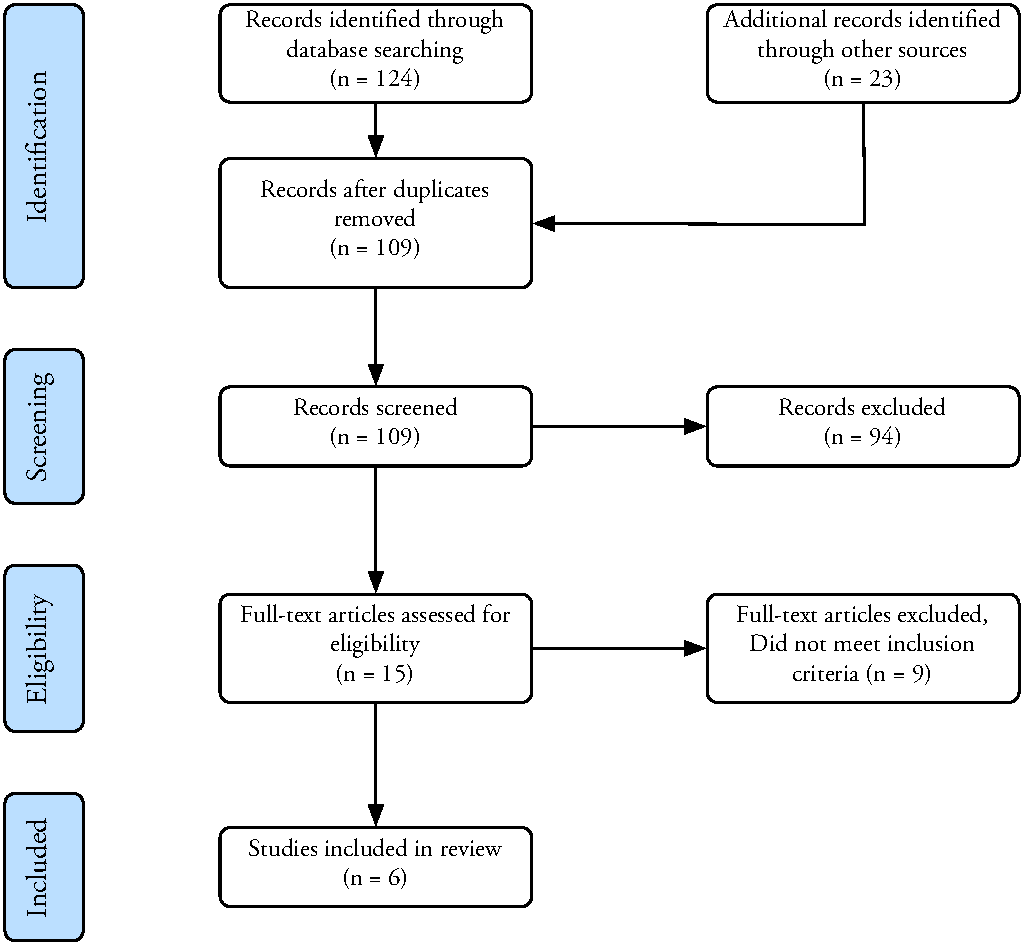
\includegraphics[keepaspectratio,width=0.9500\textwidth,height=0.75\textheight]{prismalit.pdf}
\caption{PRISMA flow diagram of search results}
\label{prismalit}
\end{figure}



\subsection{Description of studies}
\label{descriptionofstudies}

The six studies can be split into two groups, both in terms of their respective populations and methodologies. Three of the studies (Ting~\citep{ting_abstract_2009}, Selker~\citep{selker_emergency_2011} and Cantor~\citep{cantor_prehospital_2012}), included paramedics as participants and were not randomised. Instead, two were prospective diagnostic studies (Ting and Cantor) and the third, a before and after, quasi-experimental design (Selker). These studies are summarised in \autoref{tabledataextraction}.

 \renewcommand{\arraystretch}{2.0}
\newcolumntype{L}{>{\raggedright\arraybackslash}p{0.15\textwidth}}
\newcolumntype{A}{>{\raggedright\arraybackslash}p{0.24\textwidth}}
\tiny
\begin{longtable}{LAAA}
\label{tabledataextraction} \\
\caption{Summary of literature review studies (paramedic participants)} \\
\hline
\textbf{Study}&\textbf{Cantor 2012}~\citep{cantor_prehospital_2012}&\textbf{Selker 2011}~\citep{selker_emergency_2011}&\textbf{Ting 2009}~\citep{ting_abstract_2009}\\
\hline
\endfirsthead
\multicolumn{3}{l}
{\tablename\ \thetable\ -- \textit{Continued from previous page}} \\
\hline
\textbf{Study}&\textbf{Cantor 2012}&\textbf{Selker 2011}&\textbf{Ting 2009} \\
\hline
\endhead
\hline \multicolumn{4}{r}{\textit{Continued on next page}} \\
\endfoot
\hline
\endlastfoot
Population&134 consecutive patients with suspected STEMI taken for pPCI.&437 patients over three phases.&2,007 patients but only 54 patients with suspected STEMI.\\
Intervention&New protocol for primary care paramedics. Computer interpretation of 12-lead ECG (GE Marquette 12SL).&Computer interpretation using ACI-TIPI and TPI diagnostic tools. Usual computer interpretation message provided provided (GE Marquette 12SL).&Prehospital ECG protocol. Computer interpretation message provided (GE Marquette 12SL).\\
Comparison&Blinded doctor interpretation of prehospital 12-lead ECG. Final diagnosis confirmed with angiography and cardiac biomarkers.&Blinded doctor with access to patients clinical records, ECGs and cardiac biomarkers.&Diagnosis determined by angiography.\\
Outcomes&Accuracy of STEMI recognition, complications during transfer and treatment times.&Percentage of true and false positive patients identified by paramedics as having ACS or STEMI.&Accuracy of STEMI recognition by paramedics.\\
EMS system, skill level and training&Single site in Canada.  Primary care paramedics in study received 4 hours training on 12-lead ECG STEMI recognition.&11 sites throughout USA.  NAEMT certified paramedics received 4 hours training in ACS and STEMI recognition and ACI-TIPI and TPI tools.&Single site in USA.  67 NAEMT certified paramedics received 3 hours training on protocol, ECG acquisition and interpretation.\\
Results&Doctor agreed with paramedic 121\slash 134 (90\%) participants. Final diagnosis: STEMI 106\slash 134, false positive 28\slash 134. 11\slash 28 false positives could have been excluded if only computer interpretation utilised. 8 true STEMIs missed by computer interpretation.&Comparison between phase 1 and 2: STEMI identification increased from 40.8\% to 68.4\% (p$<$0.01). Retrospective analysis of ACI-TIPI and TPI gave true positive rate for STEMI as 73\%.&Prehospital recognition of STEMI: sensitivity 48.0\%, specificity 99.6\%, Positive predictive value 86.7\%, Negative predictive value 97.4\%. False negatives: 57\% due to inaccurate computer interpretation, 21\% due to cardiac arrest where no ECG recorded.\\
Notes&Primary care paramedics are equivalent to EMT-B in USA and ambulance technicians in the UK.&Training for new (to study) paramedics reduced to 1.5 hours in phase 3. Only study which utilised ACI-TIPI and TPI tools. Analysis of phases retrospective. Patients not required to have chest pain.&Only post-implementation data usable. No record of missed STEMIs not using protocol. Not clear what demographic data recorded for patients who were not in the protocol.\\
\end{longtable}
\renewcommand{\arraystretch}{1}
\normalsize 

The three remaining studies utilised doctors as participants and were randomised, utilising experimental survey designs rather than actual patient episodes (Goodacre~\citep{goodacre_computer_2001}, Massel~\citep{massel_observer_2003} and Tsai~\citep{tsai_computer_2003}). A summary of these doctor studies is provided in \autoref{tabledataextraction1}.

 \renewcommand{\arraystretch}{2.0}
\newcolumntype{P}{>{\raggedright\arraybackslash}p{0.15\textwidth}}
\newcolumntype{Q}{>{\raggedright\arraybackslash}p{0.24\textwidth}}
\tiny
\begin{longtable}{PQQQ}
\label{tabledataextraction1} \\
\caption{Summary of literature review studies (doctor participants)} \\
\hline
\textbf{Study}&\textbf{Tsai 2003}~\citep{tsai_computer_2003}&\textbf{Massel 2003}~\citep{massel_observer_2003}&\textbf{Goodacre 2001}~\citep{goodacre_computer_2001} \\
\hline
\endfirsthead
\multicolumn{4}{l}
{\tablename\ \thetable\ -- \textit{Continued from previous page}} \\
\hline
\textbf{Study}&\textbf{Tsai 2003}&\textbf{Massel 2003}&\textbf{Goodacre 2001} \\
\hline
\endhead
\hline \multicolumn{4}{r}{\textit{Continued on next page}} \\
\endfoot
\hline
\endlastfoot
Population&30 doctors (internal medical residents) in second or third year of training.&9 doctors. 3 medical residents, 3 cardiology fellows and 3 consultant cardiologists.&10 doctors, all senior house officers.\\
Intervention&23 ECGs (11 in group A, 12 in group B) with computer interpretation message.&75 ECGs with typical history, checklist and computer interpretation.&25 ECGs with computer interpretation message.\\
Comparison&23 ECGs (11 in group A, 12 in group B) with computer interpretation message hidden.&75 ECGs with atypical history, no checklist and no computer interpretation.&25 ECGs without computer interpretation message.\\
Outcomes&Interpretative accuracy of the medicine residents. Secondary outcome measure: the effect of incorrect computer interpretation.&Intra- and inter-observer variability and bias measurements.&Proportion of major errors missed in each group. Secondary outcome measure: number of completely correct ECGs, without major or minor errors.\\
Site(s)&US university department of medicine.&Single tertiary care centre in Canada.&Single emergency department in a UK teaching hospital.\\
Results&Without computer interpretation, accuracy 48.9\% (95\% CI, 45.0-52.8\%). With computer interpretation, 55.4\% (95\% CI, 51.9-58.9\%; p$<$0.0001). When the correct computer interpretation included, accuracy 68.1\% (95\% CI, 63.2-72.7\%; p$<$0.0001).  Participants wrongly agreed with incorrect computer interpretation more often when visible 67.7\% (95\% CI, 57.2-76.7\%) than when it was not 34.6\% (95\% CI, 23.8-47.3\%; p$<$0.0001).&When all doctors considered as a group, improvement in inter-observer ECG interpretation when computer message provided (p=0.0001).  Medical residents biased by computerised ECG (p$<$0.001) and less likely to recommend thrombolysis.&Major errors found in 46\slash 250 (18.4\%) ECG interpretations made by SHOs with computer interpretation visible. 56\slash 250 (22.4\%) major errors found in interpretations without computer message visible. No evidence of relationship between computer interpretation use and major errors by SHOs.\\
Notes&Computer algorithm not identified. ECGs not restricted to STEMI.&GE Marquette 12SL algorithm used. ECGs were not restricted to STEMI.&GE Marquette 12SL algorithm used. ECGs were not restricted to STEMI.\\


\end{longtable}
\renewcommand{\arraystretch}{1}
\normalsize 

\subsubsection{Paramedic studies}
\label{paramedicstudies}

The Cantor study~\citep{cantor_prehospital_2012} was a prospective diagnostic study, and enrolled 134 patients who were taken directly for pPCI at one Canadian hospital. The intervention was a newly introduced prehospital protocol, allowing primary care paramedics (PCP) to bypass local EDs in order to take patients directly to the pPCI centre. Prior to the study, PCPs received three hours training relating to 12-lead ECG interpretation.

The primary outcome was accuracy of prehospital STEMI recognition, which was compared to an experienced cardiologist who had access to the prehospital ECG, but not the angiography or cardiac biomarker results, and final diagnosis, as determined by cardiac biomarker results and angiography. Secondary outcomes included the number of complications en route and various treatment timings. In addition, computer interpretative accuracy alone, was calculated.

The Selker study~\citep{selker_emergency_2011} was a three phase, before and after quasi-experimental study, to test the use of the acute cardiac ischaemia time-insensitive predictive instrument ~\citep{selker_use_1998} and thrombolytic predictive instrument by paramedics~\citep{selker_use_2002}, to identify suitable participants for the Immediate Myocardial Metabolic Enhancement During Initial Assessment and Treatment in Emergency Care (IMMEDIATE) trial.~\citep{selker_out--hospital_2012} It was conducted in multiple sites throughout the US, with paramedics who were National Association of Emergency Medical Technicians (NAEMT) registered, and so roughly equivalent to UK paramedics. Prior to the study commencing, four hours of ECG interpretation and study tool training were provided.

The primary outcomes were proportions of patients correctly and incorrectly identified by paramedics as having an ACS, with a subsequent sub-group analysis of patients with STEMI. In addition, a retrospective analysis was conducted to determine the accuracy of the ACI-TIPI and TPI alone.

The Ting study~\citep{ting_abstract_2009} was a prospective diagnostic study conducted in the US, which collected demographic data from 2,007 patients taken by a single ambulance service to the study hospital, who were diagnosed with STEMI and underwent pPCI. The intervention was a new prehospital protocol which allowed study paramedics (NAEMT registered) to bypass the local ED and take patients directly to the study hospital's cardiac catheter lab. Prior to the start of the study, paramedics received three hours training, including familiarisation with the study protocol and 12-lead ECG acquisition and interpretation.

The primary outcome was accuracy of paramedic recognition of STEMI, which was compared to final hospital discharge diagnosis determined by ECG findings, angiography and successful reperfusion with pPCI. 

\subsubsection{Doctor studies}
\label{doctorstudies}

The Tsai study~\citep{tsai_computer_2003} was a randomised crossover controlled trial with 30 internal medicine residents from a single US university medical centre, who were in their second or third year of training. The participants were stratified according to year of training and then randomly allocated into one of two groups, which determined in which order the ECGs with computer interpretation would be viewed. Group A contained 11 ECGs and group B, 12, making a total of 23 ECGs. The study took place over a five-month period, with the ECG interpretation being conducted as a one-hour, supervised session.

The primary outcome was interpretative accuracy of the medicine residents, with a secondary outcome of the effect of incorrect computer interpretation on the participant's interpretations which were incorrect.

The Massel study~\citep{massel_observer_2003} was a two-by-two-by-two factorial randomised control trial (RCT) with nine participants from a single tertiary teaching hospital in Canada. There were three doctors from each of the following grades:

\begin{itemize}
\item Medical resident

\item Cardiology fellow

\item Consultant cardiologist.

\end{itemize}

The participants reviewed 75 ECGs, selected from the coronary care unit (CCU) and hospital patients by the researchers. Due to the factorial design, they were required to review the ECGs eight times over an eight-month period.

The primary outcome was the reliability and accuracy of ECG interpretation and the effect of three contributing factors (clinical history, a checklist developed as part of the study and computer interpretation).

The Goodacre study~\citep{goodacre_computer_2001} was an RCT with 10 participants, all junior doctors, working at a single UK teaching hospital emergency department. They reviewed 50 ECGs (half with the computer interpretation message visible and half without) at a single sitting, and under examination conditions.

The primary outcome was the proportion of major errors missed in each group, with a secondary outcome measure of the number of completely correct ECG interpretations (i.e. those without major and minor errors specified by the study design). 

\subsection{Methodological quality}
\label{methodologicalquality}

\subsubsection{Validity}
\label{validity}

All six studies had a clear research question, which conformed to the population, intervention, comparison, outcome (PICO) model. Only one of the studies~\citep{goodacre_computer_2001} was conducted in the UK, with the remainder conducted in North America (three from the US~\citep{tsai_computer_2003,ting_abstract_2009,selker_emergency_2011} and two from Canada~\citep{massel_observer_2003,cantor_prehospital_2012}). There was a clear distinction between the studies involving paramedics, which included patients with suspected acute coronary syndromes (ACS), and those with doctors as participants, which utilised previously obtained ECGs.

The eligibility criteria in the paramedic studies were typically two-fold, since both para-medics and patients were required. Skill levels were specified, with paramedics in the Selker and Ting studies having comparable qualifications to that of UK paramedics (i.e. NAEMT paramedic registration), whereas the Cantor study utilised Canadian primary care paramedics, equivalent to UK ambulance technicians, the tier below paramedics. The patients in the paramedics studies also had slightly differing eligibility criteria, with Selker and Cantor not stipulating an age limit, but specifying a requirement for patients to present with signs and symptoms of ACS, whereas the Ting study only considered the ECG criteria, and patients were only eligible for entry into the study if there was agreement between paramedic and computer interpretation. The Selker and Cantor studies also allowed local protocols and the paramedic's judgement to override the study criteria. 

A key omission in determining the accuracy of paramedic's interpretation in all studies, was the omission of patients who did not undergo pPCI at the study hospital, or, in the case of the Selker study, were not identified as having an ACS and so not enrolled. In addition, none of the studies compared paramedics’ diagnoses alone. Therefore, without the benefit of computer interpretation, differentiating the effect that paramedic and computer interpretations had on the accuracy of diagnosis is difficult to determine, even when the computer interpretation accuracy rates were reported separately.

The doctor studies all involved junior doctors (defined as being 2--3 years post-graduation), although Massel also included middle and senior grades. No information was provided about how the participants were recruited, but the randomisation strategy was clearly laid out in all studies, although none included a consolidated standards of reporting trials (CONSORT) flow diagram~\citep{schulz_consort_2010}. All participants were accounted for and none were lost to follow-up.

In the paramedic studies, it was apparent that some patients did not receive the diagnostic test and\slash or had the reference standard applied. Nine patients in the Ting study did not have a prehospital 12-lead ECG, but were subsequently taken for pPCI and included in the results as false negatives. No two-by-two table was included, although it is possible to calculate this from the sensitivity, specificity, negative and positive predictive values provided. Almost 3\% of patients in the Selker study did not have an ACI-TIPI score calculated, leading to a risk of verification bias~\citep{lijmer_empirical_1999}. A two-by-two table was not provided in the results, as only the test positive results were included. There was no missing data in the Cantor study, although one patient did not receive the reference standard test (pPCI) since the patient was considered to be a false positive and so not appropriate for pPCI.

The reference standard for the doctor studies were senior cardiologists or ED consultants, who independently reviewed the study ECGs prior to the study commencing, and who were blinded to the computer interpretation result. Their responses were collated and any disagreements were resolved by discussion. When assessing the participants' responses, only the Tsai study made it clear that the marker was blinded to the participant identity and computer interpretation message. However, the marking in this study was conducted by only one researcher. The Goldacre study blinded the assessors to the computer report, but it was not clear whether they were blinded to the participant identity. However, in contrast to the Tsai study, both ED consultants independently reviewed the participants' results and their agreement was measured by the calculation of the $  \kappa  $ statistic, with disagreements resolved by discussion. The Massel study provides no information about whether the researchers were blinded to the participant identity or the presence of the computer interpretation message, which could be a source of review bias~\citep{whiting_sources_2004}. However, the participants were blinded to their previous answers and those of fellow participants. 

All three paramedic studies used angiography and cardiac biomarkers as the reference standard for diagnosis. In addition, two of the paramedic studies (Selker and Cantor), also used a doctor with access to the patients' notes, but blinded to the paramedic's study results as an additional reference standard. The Ting study did not specify whether the research staff accessing the patients' notes were blinded.

Four of the studies utilised the GE Marquette 12SL algorithm, with the Tsai and Massel studies failing to identify the algorithm used. In addition, the Selker study also utilised two additional novel algorithms (ACI-TIPI and TPI) in the latter phases of their study.

The study procedures were clearly outlined in all studies, although in the case of the Ting study (published as a conference abstract), it was necessary to obtain a further article to review the protocol, after the lead author failed to respond to direct communication~\citep{nestler_impact_2011}. Eligibility criteria were provided for all of the paramedic studies, but little explanation was provided in the doctor studies. Baseline characteristics of patients were provided in two of the paramedics studies, with only Cantor failing to provide any demographic or co-morbidity information, making assessment of spectrum bias impossible~\citep{whiting_sources_2004}. All of the doctor studies provided current job role and years since graduation, but only Massel provided additional data about average ECG interpretations conducted by the participant per week. This was lacking in the Goodacre and Tsai studies, making it difficult to determine whether control and intervention groups were equivalent. The Tsai study describes the design as a matched pairs crossover design, but the only matching that appears to have been conducted was years since graduation. In addition, a single participant did not see the same ECG twice, once with and without the computer interpretation, but instead saw an equivalent set of ECGs for each phase. Massel used a crossover design, and participants saw the same ECG on multiple occasions, both with and without the computer interpretation. These issues aside, all of the doctor studies did treat the intervention and control arms of the studies in the same way, except for applying the intervention.

\subsubsection{Results}
\label{results}

While all three of the paramedic studies provided information about the accuracy of computer interpretation alone, it was not possible to determine the accuracy of the paramedics alone, since all were exposed to the computer interpretation when making a diagnosis. The doctor studies in comparison, thanks to their randomised control trial design, provide responses with and without the computer interpretation.

In the Cantor study, paramedics identified 134 patients as suspected STEMI and were correct in 106 (79\%) of cases. If the diagnosis had been made by computer interpretation alone, 98\slash 106 (92\%) of patients with STEMI would have been correctly identified, correctly excluding a further 11\slash 28 (39\%) of the false positives.

The three phase design of the Selker study makes analysis of the results rather more complicated. All three phases provided paramedics with computer interpretation, however in the latter phases, the criteria were amended to require an ACI-TIPI prediction of 75\% or more, or a TPI prediction of STEMI. Despite this, paramedics were still able to activate their local pPCI pathway if the local emergency medical service (EMS) protocol eligibility criteria was met. The study found a statistically significant increase in the percentage of patients with STEMI between phases 1 and 2, rising from 40.8\% to 68.4\%. However, since the study also included patients with ACS and not just STEMI, it makes direct comparison with the other paramedic studies difficult. A retrospective analysis by the researchers explored the ACI-TIPI and TPI across all three phases and found that, in cases of confirmed ACS, the computer correctly identified 226\slash 284 (80\%) of patients, compared with paramedics with computer interpretation, who correctly identified 296\slash 437 (68\%).

The Ting study was the only one to provide sufficient information to construct a two-by-two table. In addition, although study protocol required that paramedic and computer interpretation had to agree in order for the patient to be considered for direct admission to the cardiac catheter unit, patients who were taken to the study hospital and who had a final diagnosis of STEMI were also included. This made it possible to identify occurrences when the paramedic and computer disagreed. Paramedics agreed with the computer interpretation in 26\slash 54 (48.1\%) of STEMI cases. If only the paramedic's interpretation had been required, correct recognition would have increased to 43\slash 54 (79.6\%).

The Tsai study reported correct and incorrect results for computer interpretation alone, participants alone, and participants with the computer message. However, only 18\slash 54 of the study ECGs could be considered to be STEMI or STEMI-mimic in morphology, which limits the results' applicability to the RESPECT study. Results were reported as average (presumably means, although this was not stated) values. In the sub-category of correct computer interpretation, 53\% of participants correctly interpreted the ECG without the computer message, with a statistically significant increase to 68\%, when it was visible. However, when the computer interpretation was incorrect, participants were incorrect 35\% of the time when the message was hidden, rising to a statistically significant 68\% when the incorrect message was shown.

The Massel study utilised a two-by-two-by-two factorial design, requiring participants to view ECGs on four separate occasions with and without the computer interpretation, and with differing combinations clinical history and the presence (or absence) of a checklist. Results were reported using inter- and intra-class reliability measures ($  \kappa $ statistics) and tendencies of bias. Mean overcalls and undercalls for thrombolysis eligibility were also reported, including 95\% confidence intervals. Only the medical residents had statistically significant effects caused by the presence of the computer interpretation message. They were biased by the computer interpretation and more likely to undercall thrombolysis (the mean undercall rose from 5.4\% to 8.5\% in the presence of the computer interpretation message). In the sub-group of ECGs which were accompanied by a typical history of AMI, medical residents were more likely to change their decision in favour of thrombolysis if the computer interpretation was provided.

The Goodacre study consisted of 10 junior ED doctors who each interpreted 50 ECGs, 25 with a computer interpretation and 25 without. As with the Massel study, ECGs were not exclusively limited to STEMI and the breakdown of ECG findings was not reported. Interpretations were classified into three categories: completely correct, major errors and minor errors. The criteria for major errors did include ST-segment elevation of $>$1mm. Results were reported as proportions, with confidence intervals and p-values provided. Overall, the computer interpretation messages had no statistically significant effect on the participants. Major errors occurred in 46\slash 250 (18\%) of interpretations with the computer message, which rose to 56\slash 250 (22\%) without (p=0.13). Participants correctly interpreted 104\slash 250 (42\%) ECGs with the computer message and 91\slash 250 (36.4\%) without (p=0.15).

Only the Goodacre study provided a power calculation to justify the sample size chosen, but this did not account for the clustering of data in the study. In fact, none of the studies took clustering into account in the analysis of data. The Tsai study did acknowledge the multi-level nature of the data, but assumed that this would not have any effect. This is unwise, since not accounting for clustering leads to smaller standard errors (and confidence intervals), increasing the likelihood that chance findings will be considered to be statistically significant~\citep{bland_statistics_1997}. 

\subsubsection{Context}
\label{context}

The literature review has highlighted the absence of studies directly examining the effect of computer interpretation messages on paramedic's recognition of STEMI. The paramedic studies identified in the review do have a clinically relevant context, but the lack of results of paramedic interpretation alone, makes it impossible to isolate the effect of the computer interpretation. The studies do suggest that computer interpretation has an effect, but not whether this is clinically significant.

The doctor studies are able to determine the effect of computer interpretation alone, however, this is a distinctly different population to paramedics, and the results of the studies lack generalisability, due to the small numbers of participants. In addition, ECG interpretation was not limited to STEMI or STEMI-mimics in two of the studies (Goodacre and Tsai), further reducing their applicability to the research question. This is compounded by the failure to account for the clustering effects of the data.

Only one of the studies was based in the UK (Goodacre, a doctor study), and one of the paramedic studies was conducted with paramedics who have a skill equivalent of ambulance technicians in the UK.

In conclusion, the methodology of the doctor studies provides a good indication about how this research question could be answered if the correct population is identified. Thus, a sufficiently powered randomised crossover trial with UK paramedics would provide an sound basis on which to answer the research question for this dissertation.
 % Lit Review - 3529 words

\chapter{RESPECT study and pilot}
\label{respectstudyandpilot}

 \lhead{\emph{RESPECT study and pilot}} % Chapter title for thesis template 

Given the doubt surrounding the effect of computer interpretation on paramedic accuracy in recognising STEMI, and the importance of minimising false positives and negatives, this study will focus on the effect that computer interpretation has on a paramedic's accurate recognition of STEMI. From the literature review, it is clear that the study design needs to take account of clustering. However, in the absence of existing studies to provide insight into intra-class correlation coefficients to determine design effects, a pilot study is necessary. In addition, the pilot provides an opportunity to test a customised, web-based assessment tool, which will record the paramedic participant's ability to correctly diagnose STEMI and exclude STEMI-mimics, both with and without a computer message, using a randomised crossover design~\citep{arain_what_2010}. 

\section{Aims and objectives}
\label{aimsandobjectives}

Pilot study aims: 

\begin{itemize}
\item To create and test a web-based assessment tool, suitable to address the main study aim

\item To determine the feasibility of the main study.

\end{itemize}

 \clearpage 

Pilot study objectives:

\begin{itemize}
\item Source at least 48 ECGs, with a proportional mix of STEMI and STEMI-mimic patterns, all with computer diagnostic messages

\item Obtain a gold-standard diagnosis of each ECG

\item Create custom database-driven website to administer the study

\item Conduct the pilot study to:

\begin{itemize}
\item Determine recruitment rates and identify incentives to minimise attrition in the main study

\item Check the randomisation procedure

\item Test that the assessment tool works correctly

\item Obtain preliminary estimates of the accuracy, sensitivity and specificity of paramedic's interpretation, to determine whether it is appropriate to conduct the main study

\item Estimate intra-class correlation coefficients for participants and ECGs, and the number of discordant proportions, in order to provide guidance in determining the sample size for an appropriately powered main study

\item Construct a generalised linear model to determine the odds ratios relating to paramedics accuracy in recognising STEMI, taking into account the clustering of participant responses and ECG.

\end{itemize}

\end{itemize}

Main study aim: To examine the effect of computer interpretation messages printed on ECGs on the accuracy of paramedics’ recognition of STEMI.

Objectives:

\begin{itemize}
\item Estimate an appropriate sample size to ensure the study is adequately powered, taking into account the clustering of data

\item Recruit paramedics from Yorkshire Ambulance Service to take part in the study

\item Obtain precise estimates of the accuracy, sensitivity and specificity of paramedic's interpretation

\item Estimate the effect of computer-generated messages on paramedic interpretation (overall and
stratified by correct and incorrect computer interpretation)

\item Disseminate the results.

\end{itemize}

\section{Value of this research}
\label{valueofthisresearch}

The results from this pilot study will demonstrate whether an online assessment tool can appropriately test paramedics' accuracy in STEMI recognition. The estimation of intra-class correlation coefficients will help determine appropriate sample sizes for an adequately powered, main study. In addition, the publication of the pilot data will also assist other researchers conducting studies in this area, given the paucity of published studies relating to this topic.

Assuming that the main study is feasible, the results will provide information about the effect that computer interpretation messages has on paramedics' recognition of STEMI. This should assist ambulance services determine whether computer interpretation should continue to be provided to their paramedics and provide insight into the current interpretation accuracy of UK paramedics. 
 % RESPECT study and pilot - 522 words

\chapter{Research methods}
\label{researchmethods}

 \lhead{\emph{Research methods}} % Chapter title for thesis template 

\section{Study design}
\label{studydesign}

This pilot study is a randomised crossover trial, utilising a bespoke, \href{http://respect.ambulanceresearch.co.uk}{web-based assessment tool}\footnote{\href{http://respect.ambulanceresearch.co.uk}{http:/\slash respect.ambulanceresearch.co.uk}} to enrol participants, randomise them appropriately, and track their progress through the study. The pilot has been designed to mirror the main study, enabling the testing of the assessment tool, data collection and analysis methods, and the statistical methods required for hypothesis testing.

\section{12-lead electrocardiograms}
\label{leadelectrocardiograms}

A key component of the assessment tool is a database of 48 12-lead ECGs showing a STEMI or STEMI-mimic waveform morphology. These are classified into four categories, based on the computer interpretation message on the ECG: true positive, true negative, false positive and false negative, when compared to the reference standard for ECGs in this study. Note that there are 12 ECGs for each classification.

\subsection{Reference standard}
\label{referencestandard}

In order to qualify for inclusion in the study, the ECGs had to meet the following reference standard set for the study:

\begin{itemize}
\item The ECG had to be a 12-lead ECG recorded in the out-of-hospital environment

\item The ECG had to display a wave morphology consistent with either a STEMI or STEMI-mimic, and a computer diagnostic message printed on the ECG.

\item The diagnosis of the ECG (i.e. STEMI or not-STEMI) had to be determined by the independent assessment and agreement of two senior doctors with specialist knowledge of ECGs. Any disagreements on diagnosis were resolved by discussion between the doctors. An option for subsequent review by an independent third party, was provided, but not required.

\end{itemize}

Information relating to the 48 ECGs that met the reference standard and were included in the pilot study, can be found in \autoref{appendixa}. 

\section{Participants}
\label{participants}

Participants for the pilot study were Health and Care Professions Council (HCPC) registered paramedics working in the United Kingdom, but not employed with Yorkshire Ambulance Service NHS Trust at the time of the study. The main study, planned to commence once the pilot data has been completed, will consist of Yorkshire Ambulance Service paramedics only. Approval has already been granted by the Service research and development department for the main study (\autoref{appendixc}). 

\section{Recruitment}
\label{recruitment}

A number of strategies were employed to recruit the target number of paramedics into the study. Firstly, the study was advertised on the \href{https://www.collegeofparamedics.co.uk/}{College of Paramedics website}\footnote{\href{https://www.collegeofparamedics.co.uk/}{https:/\slash www.collegeofparamedics.co.uk\slash }} (with the support of the College Research and Development Advisory Committee). In addition, paramedics were notified about the study via the \href{http://www.ukambulanceforum.com}{UK Ambulance Forum}\footnote{\href{http://www.ukambulanceforum.com}{http:/\slash www.ukambulanceforum.com}}, an online \href{http://www.resuscitate.me.uk}{continuing professional development portfolio builder}\footnote{\href{http://www.resuscitate.me.uk}{http:/\slash www.resuscitate.me.uk}} for ambulance staff, social media outlets such as \href{http://www.twitter.com}{Twitter}\footnote{\href{http://www.twitter.com}{http:/\slash www.twitter.com}}, email and word of mouth. 

\section{Ethical concerns}
\label{ethicalconcerns}

The confidentiality of the participants was maintained primarily through anonymity. The only potential source of personally identifiable data, the participant's email address, was encrypted on the pilot study database using a Rijndael 256-bit cypher and was not known to the researcher. In addition, there was no personal contact between participants and the researcher during the pilot study, since the website handled all communication with the participant, such as sending out reminder emails, for example. Access to the study database was limited to the chief investigator only. Once the study was completed, participants' email addresses and data were removed within one calendar month, unless express consent had been obtained from a participant to be contacted about involvement in a subsequent study.

The HCPC standards of conduct, performance and ethics, states that paramedic (and other) registrants must act in the best interests of service users, which includes reporting on the conduct, performance and health of colleagues if there is a cause for concern~\citep{health_and_care_professions_council_standards_2008}. This raised a potential ethical issue within the RESPECT pilot study, since paramedic participants' ability to interpret ECGs was tested, and since the chief investigator is a registrant of the HCPC, a dilemma about whether to report poorly performing participants arose. In actuality, since participants' identities were anonymised, and no overall score for an individual participant was calculated, it was not possible identify poorly performing participants individually.

Since the study was not conducted on NHS patients, there was no need for NHS research ethics committee (REC) approval as this is not required for research conducted on NHS staff~\citep{nhs_research_ethics_service_does_2012}. However, the study was approved by the University of Sheffield ethics committee (\autoref{appendixd}), and the University acted as the study's research governance sponsor (\autoref{appendixe}). In addition, a risk assessment was conducted, in keeping with University policy (\autoref{appendixf}). 

\section{Informed consent}
\label{informedconsent}

Participants in the RESPECT study consented online. Although, arguably, this raised an issue of ensuring that the participants were fully informed, comprehensive participant information was provided on the website (\autoref{appendixg}). Obtaining consent in this way, meant that no pressure to enrol in the study was exerted on the participant, which can occur in face-to-face consenting methods~\citep{fielding_handbook_2008}. Participants who submitted the consent form webpage (\autoref{consentform}), were considered to have provided informed consent. Additional consent was also obtained for the use of anonymised data from the study to be used in subsequent research, and for participants to be contacted for potential enrolment into a subsequent, qualitative study. These were both optional and not required to participate in the pilot.

\begin{figure}[htbp]
\centering
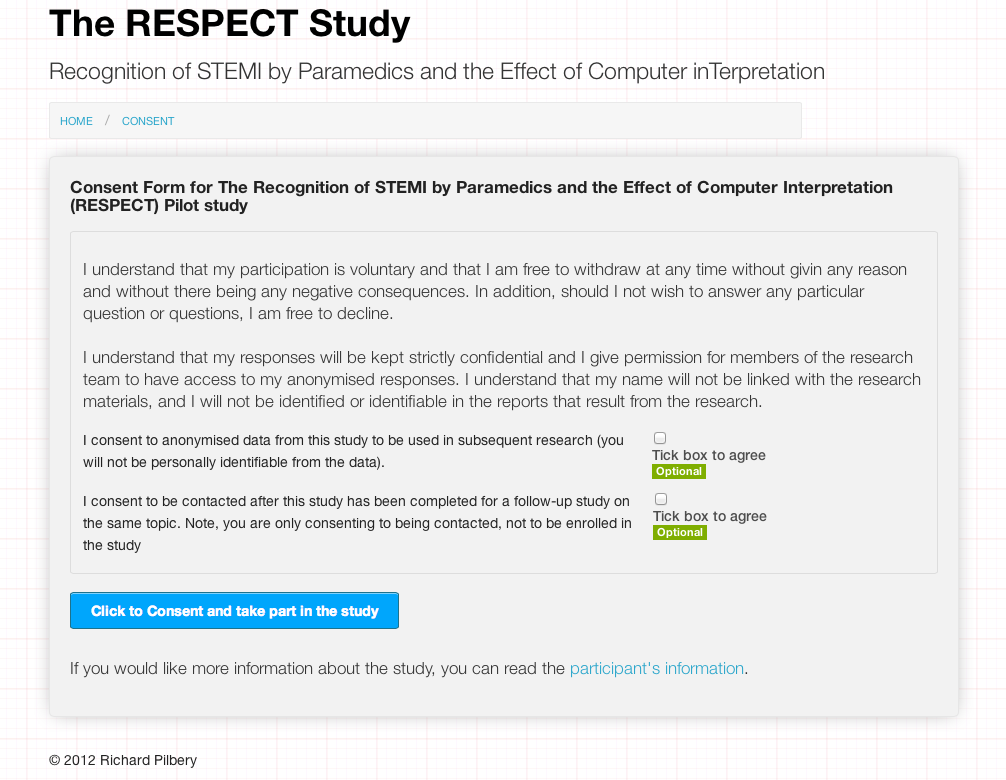
\includegraphics[keepaspectratio,width=1.0000\textwidth,height=0.75\textheight]{consent-screen.png}
\caption{Online consent form for RESPECT pilot study}
\label{consentform}
\end{figure}



\section{Research tool}
\label{researchtool}

Since it was anticipated that participants would be geographically dispersed, an online assessment tool was identified as the most efficient method to collect the data. Existing services were examined, including \href{http://www.surveymonkey.com}{Survey Monkey}\footnote{\href{http://www.surveymonkey.com}{http:/\slash www.surveymonkey.com}} and the forms tool in the \href{http://docs.google.com}{Google Docs}\footnote{\href{http://docs.google.com}{http:/\slash docs.google.com}} suite, but none met the needs of the study. Instead, a custom website was created by the researcher, coded using a \href{http://php.net}{PHP}\footnote{\href{http://php.net}{http:/\slash php.net}} framework, \href{http://cakephp.org}{cakePHP}\footnote{\href{http://cakephp.org}{http:/\slash cakephp.org}}, with a \href{http://www.mysql.com}{MySQL}\footnote{\href{http://www.mysql.com}{http:/\slash www.mysql.com}} database to record and collate the data. To ensure maximum browser and device capability, the Zurb \href{http://foundation.zurb.com}{Foundation}\footnote{\href{http://foundation.zurb.com}{http:/\slash foundation.zurb.com}} responsive front-end framework was used.

In an effort to make the ECGs used in the study as life-size as possible, participants were not permitted to use mobile devices, such as smart phones and tablets, to undertake the study. The study tool calculated the correct size to display the ECGs, based on the participant's computer screen size and resolution. This was achieved by asking participants to resize a virtual bank card displayed on the screen, to a real bank or ID card that they placed on the screen (\autoref{calibrationscreen}). Once this was submitted by the participant, the correct dimensions of the ECG image were calculated.

\begin{figure}[htbp]
\centering
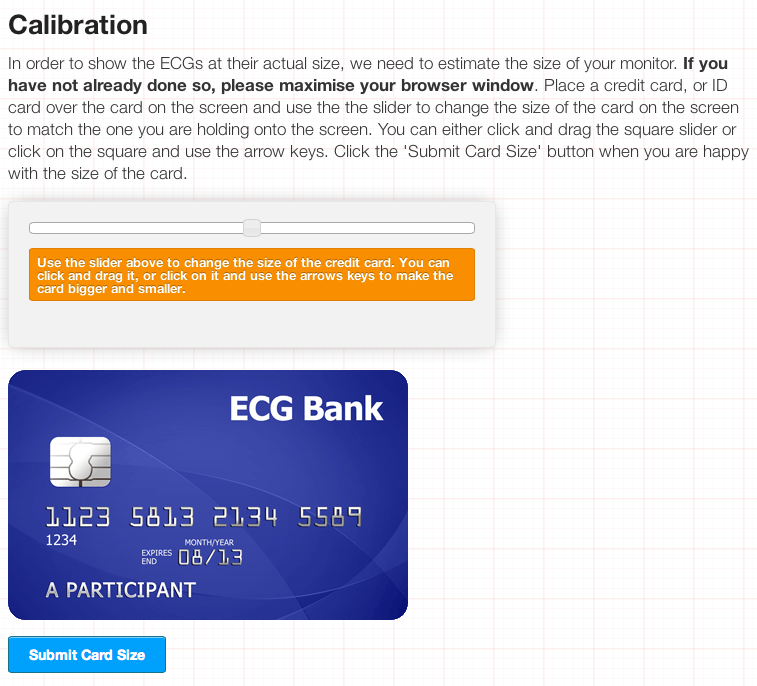
\includegraphics[keepaspectratio,width=1.0000\textwidth,height=0.75\textheight]{calibration.png}
\caption{The RESPECT study calibration screen}
\label{calibrationscreen}
\end{figure}



\subsection{Randomisation}
\label{randomisation}

The study website obtained random numbers from the true random number service \href{http://www.random.org}{RANDOM.ORG}\footnote{\href{http://www.random.org}{http:/\slash www.random.org}}, which generates random numbers from atmospheric noise. These were then utilised by the website to allocate ECGs to participants, to determine ECG and message visibility order, and determine the block randomisation sequence. 

\section{Procedure}
\label{procedure}

The participant flow through the study is shown in \autoref{partsummary}. Paramedics interested in taking part in the pilot study, were invited to visit the study website, read the participant information and enter a contact email address on the sign-up form. Once completed, the website created an entry for the potential participant and sent them an email containing a unique uniform resource locator (URL) web link, as well as links to the participant information sheet and webpage. When the participant clicked the link within the email, they were directed to the consent page (\autoref{consentform}), where informed consent was considered to have been obtained once participants submitted the consent form. Participants were also asked to optionally consent to the use of their anonymised data in subsequent research, and to be contacted about becoming involved in a future, qualitative, study.

\begin{figure}[htbp]
\centering
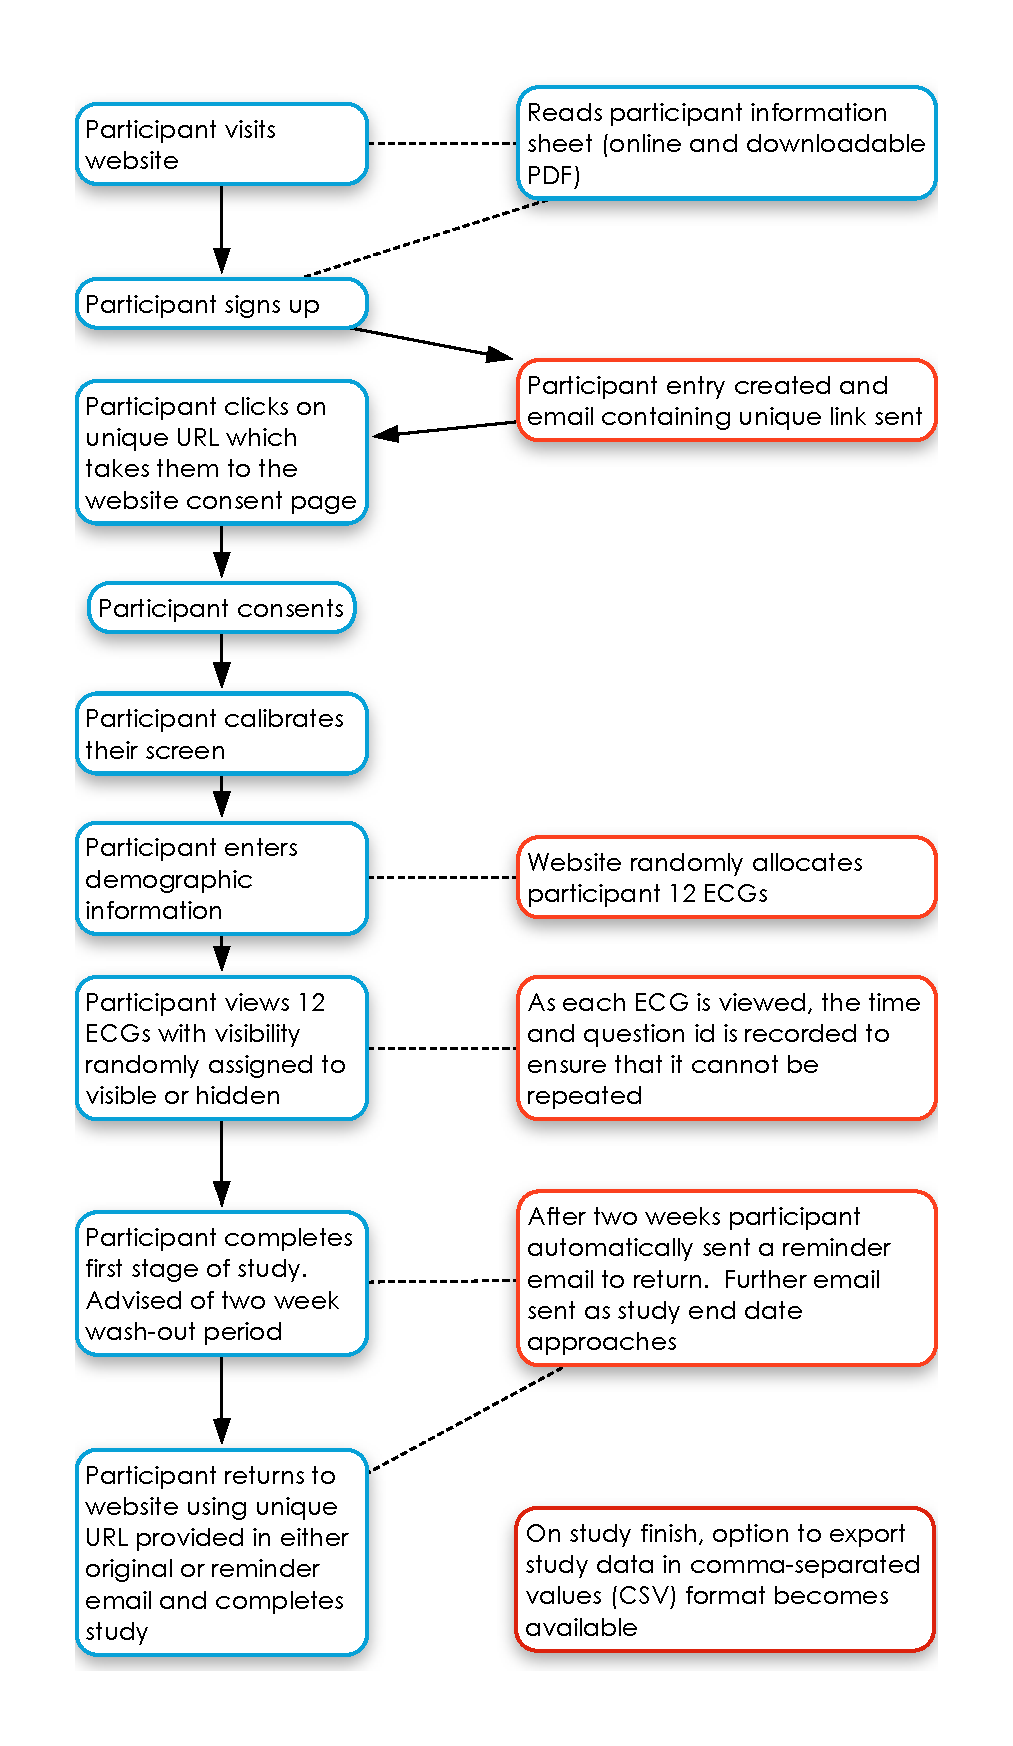
\includegraphics[keepaspectratio,width=\textwidth,height=0.9900\textheight,]{Participant-flow.pdf}
\caption{Flow of participant and website actions during the study}
\label{partsummary}
\end{figure}



After consenting, the participants calibrated their monitor. If the website was accessed using a tablet or mobile device, participants were informed that this could not be used to complete the study, and they were advised to use a desktop or laptop computer. 

The next step was to gather some basic demographic data about the participants, which took the form of four questions:

\begin{enumerate}
\item Which educational route did you take to become a paramedic (traditional\slash vocational, university)

\item How long have you been a paramedic (in years)?

\item How much time have you spent on 12-lead ECG training\slash continuous professional development (CPD) in the past 12 months (in hours)?

\item How many patients have you taken for primary percutaneous coronary intervention or thrombolysed in the past 12 months?

\end{enumerate}

Once completed, participants were randomly allocated 12 ECGs from the study pool of 48. These included three ECGs from each of the following four sub-groups:

\begin{itemize}
\item Patient has a STEMI and computer interpretation states STEMI (true positive)

\item Patient does not have a STEMI and computer interpretation states STEMI (false positive)

\item Patient has a STEMI and computer interpretation states no STEMI (false negative)

\item Patient does not have a STEMI and computer interpretation states no STEMI (true negative).

\end{itemize}

Note that the terms in brackets (e.g. true positive) refer to the computer interpretation in relation to the reference standard.

The ECGs were displayed on a pop-up webpage (\autoref{ecgform}), complete with countdown timer and a form to record the participant responses.

\begin{figure}[htbp]
\centering
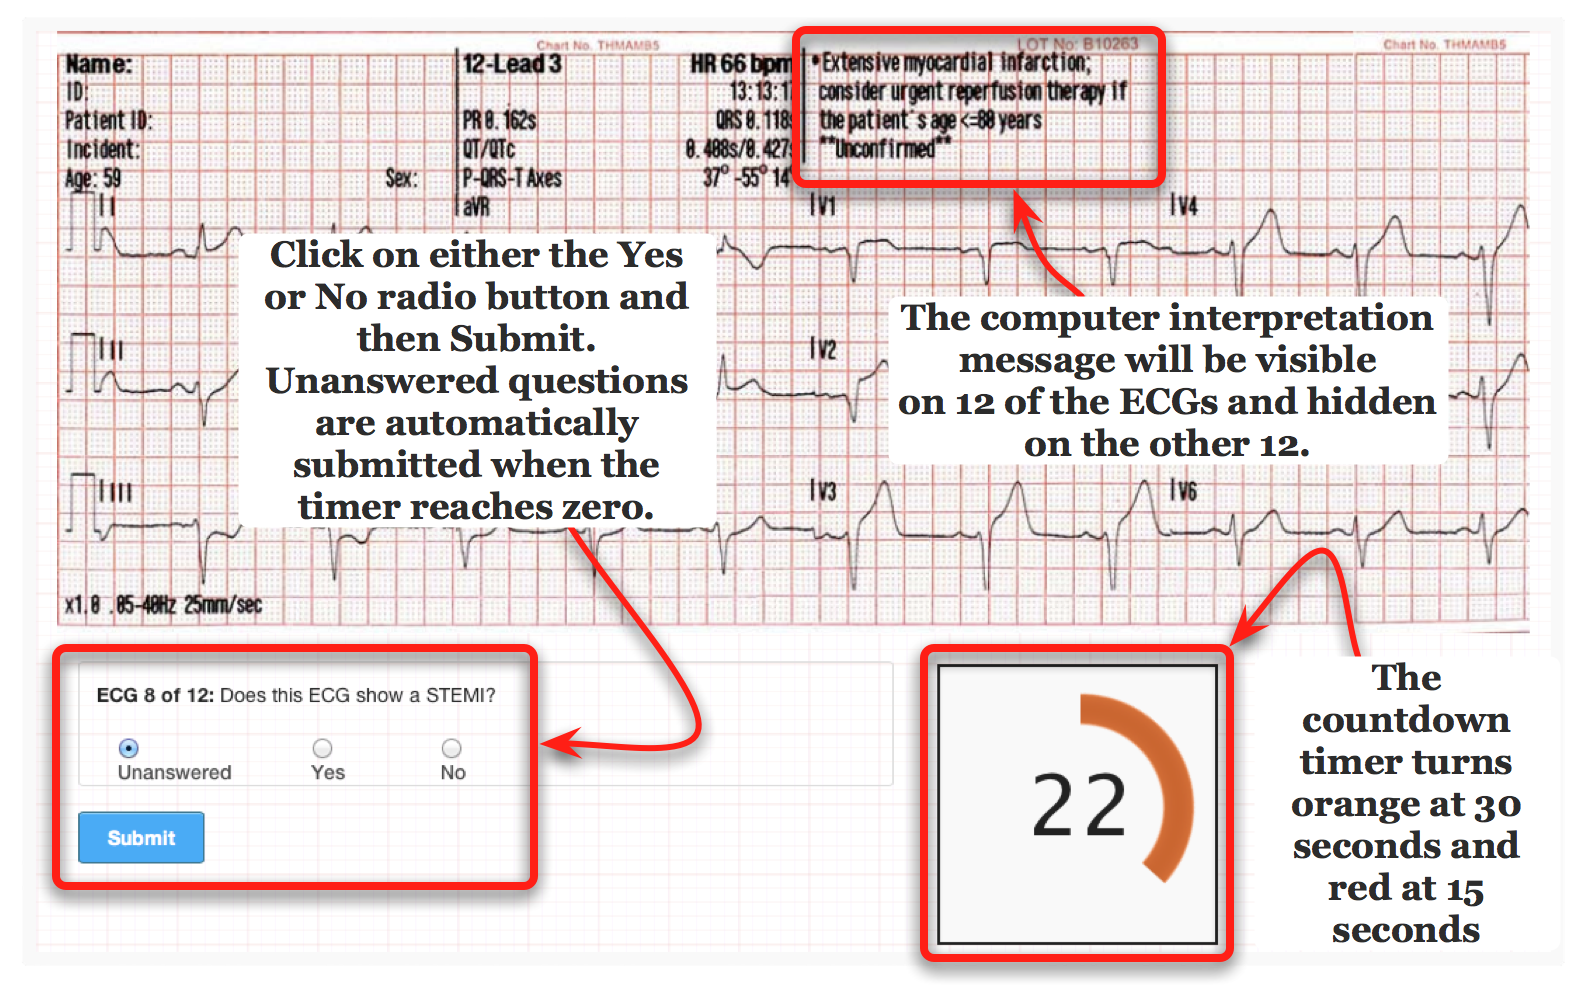
\includegraphics[keepaspectratio,width=1.0000\textwidth,height=0.75\textheight]{ecg-explain.png}
\caption{The RESPECT study ECG webpage}
\label{ecgform}
\end{figure}



Each ECG was viewed by the participant twice, once with and without the message, and the order that these ECGs were shown, was randomised. Participants were informed that the ECGs would be a mixture of STEMI and STEMI-mimic patterns, but not how many of each would be seen. In addition, they were advised that after the wash-out period, they would see the same ECGs again, but with the message visibility reversed. Incentives for completion were randomised in the pilot study, with participants either offered a CPD certificate, entered into a prize draw to win an paramedic textbook, or nothing.

To ensure that all ECGs were viewed in roughly equal numbers, block randomisation of the ECGs was used~\citep{sedgwick_block_2011}. This meant that all 48 ECGs were allocated after every forth participant, assuming that they completed the study. To minimise the chance of subversion bias, allocation was completely automated and the researcher unaware of the randomisation sequence~\citep{torgerson_designing_2008}.

Once the allocation of ECGs was completed, participants were presented with 12, 12-lead ECGs, each having a time limit of 60 seconds to interpret the ECG and submit a response. As soon as an ECG was displayed on the participant's screen, the record for that attempt was updated and no subsequent attempt was allowed, even if the participant failed to answer the question. After 60 seconds, or on submission of the form on the page, the ECG and submission form were removed from the screen and the participant was invited to view the next ECG. 

Once the first 12 ECGs had been reviewed, participants were given a two-week wash-out period and not allowed to progress until this time period had elapsed. Once the wash-out period was over, participants were contacted by email and invited to take part in the second phase (i.e. the crossover). Participants reviewed the same 12 ECGs as before, but in a random order, and with the computer message visibility the opposite of that viewed in the first phase. 

\section{Analysis plan}
\label{analysisplan}

\subsection{Data checking}
\label{datachecking}

Prior to analysing the results, the data was checked to ensure that categorical data (training route and the ECG answers) had allowed values, and numerical variables (CPD hours, service years, number of thrombolysis\slash pPCI patients) were within appropriate ranges. In addition, question start and finish times were reviewed to ensure that finish times occurred after start times. 

\subsection{Missing data}
\label{missingdata}

Due to the crossover nature of the design, each ECG viewed by an individual participant should have a paired response. Where this did not occur, the responses for the specific individual were excluded. This was on the basis that the data were unlikely to be missing at random and the statistical analysis required to account for this is well beyond the capabilities of a non-statistician~\citep{ho_dropouts_2012}. In addition, continuing with the analysis on the assumption that the data was missing at random would have resulted in bias~\citep{baraldi_introduction_2010}.

Responses which timed out (i.e. were not answered within 60 seconds) were coded differently in order to differentiate them from active participants responses. However, for the analysis, these were treated as providing an incorrect answer on the basis that a delayed response reflected the participant's uncertainty regarding the interpretation. 

\subsection{Data description}
\label{datadescription}

Since the data were clustered around participants (who viewed multiple ECGs) and ECGs (which were viewed by multiple participants), a modified Consolidated Standards of Reporting Trials (CONSORT) flow diagram~\citep{campbell_consort_2012} was created to clearly identify participant flow through the study, and provide summary information for the ECGs, including details about the characteristics of the clusters. 

\subsection{Participants}
\label{participants}

As part of the consenting process, participants were asked if they were prepared to allow their anonymised data to be used in future studies, and for permission to contact them for a subsequent, qualitative study. Since the demographic-type data collected from participants was not expected to be normally distributed, it was summarised using median values. 

\subsection{Electrocardiograms}
\label{electrocardiograms}

Two summary tables containing participant responses for each of the ECGs was created to provide overall completion rates for individual ECGs and a descriptive analysis of the responses. These tables are best utilised alongside the summary ECG data in \autoref{appendixa}, which provides the characteristics of the ECGs themselves, including the classification and the actual, and computer, interpretation. 

\subsection{Data analysis}
\label{dataanalysis}

Statistical data analysis was conducted using the \href{http://www.r-project.org}{R}\footnote{\href{http://www.r-project.org}{http:/\slash www.r-project.org}} statistics package and proceeded in an incremental fashion, commencing with the calculation of participant accuracy, sensitivity and specificity values and intra-class correlation coefficients, before fitting generalised linear regression models (GLM) with and without random effects (multilevel) modelling, to take account of the clustering of data around the participants and ECGs~\citep{petrie_medical_2000}. Although it is not possible to analyse the results of these models, due the lack of \emph{a priori} power calculations, it provided an opportunity to test the analysis methods that will be adopted in the main study. The results of the GLM analysis were verified with another statistics package, \href{http://www.bristol.ac.uk/cmm/software/mlwin/}{MLWin}\footnote{\href{http://www.bristol.ac.uk/cmm/software/mlwin/}{http:/\slash www.bristol.ac.uk\slash cmm\slash software\slash mlwin\slash }}, using the procedure described in \autoref{appendixb}.

\subsubsection{Hypotheses}
\label{hypotheses}

The following hypotheses are to be tested in the main study, and so were tested in the pilot study, to ensure that accurate data preparation and analysis could be conducted:

\begin{quote}

Null hypothesis \textbf{1} - Computer interpretation messages have no effect on paramedics' correct diagnosis of STEMI from a 12-lead ECG 

Alternative hypothesis \textbf{1} - Computer interpretation messages have an effect on paramedics' correct diagnosis of STEMI from a 12-lead ECG.
\end{quote}

The first hypothesis includes all computer interpretation messages, irrespective of classification (true positive, false positive etc). However, the subsequent hypotheses (2 and 3), aim to examine two subsets of the data: accurate (true positive and true negative) and inaccurate (false positive and false negative) computer interpretations: 

\begin{quote}

Null hypothesis \textbf{2} - \emph{Accurate} computer interpretation messages have no effect on paramedics' correct diagnosis of STEMI from a 12-lead ECG 

Alternative hypothesis \textbf{2} - \emph{Accurate} computer interpretation messages have an effect on paramedics' correct diagnosis of STEMI from a 12-lead ECG

Null hypothesis \textbf{3} - \emph{Inaccurate} computer interpretation messages have no effect on paramedics' correct diagnosis of STEMI from a 12-lead ECG 

Alternative hypothesis \textbf{3} - \emph{Inaccurate} computer interpretation messages have an effect on paramedics' correct diagnosis of STEMI from a 12-lead ECG.
\end{quote}

\subsubsection{Generalised linear modelling}
\label{generalisedlinearmodelling}

Regression models that require a transformation (via a link function) of the outcome are known as generalised linear models (GLM). For the binary outcome of a correct (or incorrect) diagnosis, logistic regression was used. Logistic regression is so called because the link function is the logit (or log odds)~\citep{kirkwood_essential_2003}. Thus the first model to be tested (which ignores the clustering of ECGs and participants) takes the form:

\[  logit(\pi) = log\left(\frac{\pi}{(1-\pi)}\right)=\beta_0+\beta_1MESSAGE \] 

where $ \pi $ is the probability of a correct answer when the message is visible, $ \beta $s are the regression coefficients and MESSAGE denotes whether the message is visible (1) or hidden (0)~\citep{campbell_medical_2007}. All data and sub-groups, consisting of accurate computer interpretation only and inaccurate computer interpretation only, were modelled. The Odds ratio, regression coefficient standard error and 95\% confidence interval, z statistic and p-values were calculated and summarised. 

\subsubsection{Generalised linear modelling with random effects}
\label{generalisedlinearmodellingwithrandomeffects}

Regression modelling assumes that the outcome and parameters are independent and identically distributed~\citep{goldstein_multilevel_2002}. However, that is not the case in this study, as each participant response is clustered around the participant and the ECG. Ignoring clustering generally leads to underestimation of regression coefficient standard errors, which in turn leads to overly narrow confidence intervals, and p-values which are too small. Ultimately, coefficients could erroneously be assumed to be significant effects, when in fact the results occurred by chance~\citep{clements_using_2007}.

Clustering can be accounted for by adding random effects to the model. This is achieved by the inclusion of a parameter which varies randomly between clusters, and is assumed to be normally distributed with a mean zero, and a variance equal to the intra-parameter variance. Including random effects in this way, allows observations within the same cluster to be assumed to be independent. Models using random effects are often called multi-level models, since the observations (a participant's individual response to a single ECG) is nested within clusters of the participant and ECG.

The participants and the ECGs are nested within a hierarchy, with each participant response belonging to a participant and an ECG. This is known as a cross-classified structure~\citep{leckie_cross-classified_2013} and can be expressed, using classification notation~\citep{browne_multiple_2001}, as:

$   y_i \thicksim Binomial(1,\pi_i)  $

$ logit(\pi_i) = \beta_0+\beta_1MESSAGE_i+u^{(3)}_{ecg(i)}+u^{(2)}_{participant(i)} $

$  u^{(3)}_{ecg(i)} \thicksim N\left(0,\sigma^2_{u(3)}\right)  $

$   u^{(2)}_{participant(i)} \thicksim N\left(0,\sigma^2_{u(2)}\right)  $

where $  u^{(3)}_{ecg(i)} $ is the random effect for ecg(i), and is assumed to be normally distributed with a mean of zero and variance, $ \sigma^2_{u(3)} $. Likewise, $  u^{(3)}_{participant(i)} $ is the random effect for participant(i), and is assumed to be normally distributed with a mean of zero and variance, $ \sigma^2_{u(2)} $.

\subsubsection{Intra-class correlation coefficients}
\label{intra-classcorrelationcoefficients}

The intra-class correlation coefficient (ICC) is a measure of the degree of similarity in ECG interpretation attempts within a cluster~\citep{eldridge_intra-cluster_2009}, and is used to calculate the design effect, by which sample size estimates are multiplied, in order to account for clustering~\citep{yelland_adjusted_2011}.

Three ICCs were calculated from the random effects models. The first, examined the correlation between two randomly selected responses from the same participant:
\[ \frac{\sigma^2_{participant}}{\left(\sigma^2_{ecg}+\sigma^2_{participant}+\frac{\pi^2}{3}\right)} \]

The second ICC, measured the correlation between two randomly selected responses from the same ECG:
\[ \frac{\sigma^2_{ecg}}{\left(\sigma^2_{ecg}+\sigma^2_{participant}+\frac{\pi^2}{3}\right)} \]

Finally, the correlation between two randomly selected responses from the same participant, and same ECG (sometimes called the interaction ICC) was calculated:
\[ \frac{\sigma^2_{ecg}+\sigma^2_{participant}}{\left(\sigma^2_{ecg}+\sigma^2_{participant}+\frac{\pi^2}{3}\right)} \]

In all cases, $  \sigma^2_{participant} $ is the variance between participants, $  \sigma^2_{ecg} $ the variance between ECGs and $  \frac{\pi^2}{3} $ is the residual variance for a logit model. 

\subsubsection{Incentives}
\label{incentives}

Participants who consented to take part in the study were randomly assigned one of three incentive options (no incentive, a downloadable continuing professional development certificate and a prize draw for a paramedic textbook). A participant was eligible for the incentive IF they completed both parts of the study. To determine the potential impact of offering incentives on retention, the following hypothesis was proposed:

\begin{quote}

Null hypothesis \textbf{4} - The proportion of study completion does not differ between the incentive options

Alternative hypothesis \textbf{4} - The proportion of study completion is different between the incentive options.
\end{quote}

This was tested using a chi-squared test for independence. 

\section{Limitations and potential problems}
\label{limitationsandpotentialproblems}

Since this study is a pilot, the results, will require confirmation in a subsequent study~\citep{torgerson_designing_2008}. No clinically important results were determined prior to the study commencement, which means that an appropriate sample size calculation to improve statistical rigour, was not calculated.

Recruiting participants was anticipated to be a significant problem~\citep{watson_increasing_2006}. Although there was an incentive, it could not be advertised, since 1 in 3 participants were not going to receive one. Given that there was no budget for marketing, social networking tools were utilised, including \href{http://twitter.com}{Twitter}\footnote{\href{http://twitter.com}{http:/\slash twitter.com}}, the \href{http://www.ukambulanceforum.com}{UK Ambulance Forum}\footnote{\href{http://www.ukambulanceforum.com}{http:/\slash www.ukambulanceforum.com}} and personal contacts throughout the UK. In addition, support was obtained from the College of Paramedics who advertised the study on the \href{https://www.collegeofparamedics.co.uk/home/}{College website}\footnote{\href{https://www.collegeofparamedics.co.uk/home/}{https:/\slash www.collegeofparamedics.co.uk\slash home\slash }}.

There was a risk that the web-based assessment tool could prove difficult to use and\slash or suffer from technical glitches, making data collection problematic. However, the tool was extensively tested prior to the start of the pilot to ensure it captured data reliably. Furthermore, limited usability testing on paramedics who were not taking part in the pilot study was undertaken to ensure that the instructions were clear and the assessment tool straightforward to use. These issues are precisely why conducting a pilot study is a good idea, and should ensure that the tool is robust enough for use in the main study.

With a web-based assessment tool, there was a risk that the participant might have utilised a textbook or sought advice from others. In order to minimise this, a unique universal resource locator (URL) was included in the emails sent to each participant, preventing unauthorised access to the study website. In addition, each ECG, once viewed by the participant, could not be answered again, and a time limit was imposed for each question, after which the website automatically removed the ECG and the response form from view.

The study's crossover design required participants to return to the website, to repeat the assessment, two weeks after completing the first stage. This did present an issue, since if participants did not return, then there would be no paired data to analyse. In an effort to minimise this, automatically generated emails were sent to participants, reminding them to return to the study, and the aforementioned social networks were utilised in an ongoing effort not just to recruit new participants, but also to encourage existing participants to return after the wash-out period.

\section{Methods of dissemination}
\label{methodsofdissemination}

The results of the study are presented and discussed in detail in \autoref{results}. Since consent was obtained from participants to use an anonymised version of the dataset in subsequent research, the data will be made publicly available online, via the study website, to promote data sharing~\citep{ross_importance_2012}. However, in an attempt to reduce the likelihood of post-hoc data analysis (data-dredging)~\citep{lord_multiple_2004}, researchers who wish to access the study data will be required to submit a study protocol to the RESPECT chief investigator. In addition, to enable the research to be reproducible, a full summary of the statistical analysis will be presented using the R statistics package \href{http://yihui.name/knitr/}{knitr}\footnote{\href{http://yihui.name/knitr/}{http:/\slash yihui.name\slash knitr\slash }}, which enables a researcher to present the R scripts which conduct the analysis, and the results of that analysis, together (an example can be found in \autoref{appendixi}). More conventional methods of dissemination will also be utilised, including publishing findings in a peer-reviewed journal, such as the \emph{Emergency Medicine Journal}, presenting at conferences, and the publication of plain English summaries in the College of Paramedics newsletter and free ambulance magazines. 

\section{Timetable}
\label{timetable}

\autoref{gantt} shows the planned timeline for the RESPECT pilot study, which commenced in September 2012 and finished with the dissertation write up and submission towards the end of September, 2013. Regular meetings were scheduled with the dissertation supervisor. In addition, a statistician was periodically consulted during the design and analysis stages.

 \begin{figure}[htbp] 

 \centering 

 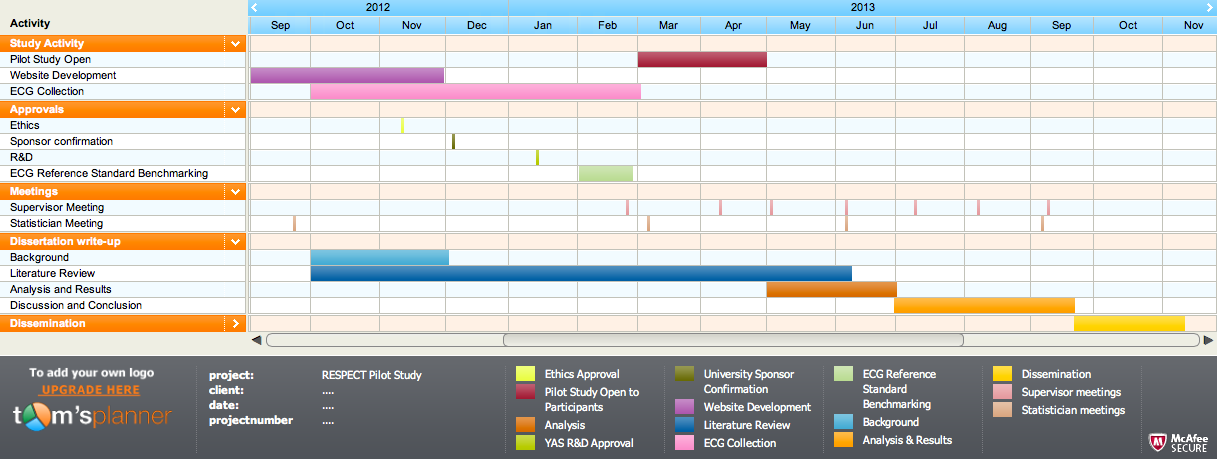
\includegraphics[keepaspectratio,width=1.50\textwidth,height=1.00\textheight, angle=90]{Gantt.png}  

 \caption{Gantt chart for RESPECT pilot study}  

 \label{gantt}  

 \end{figure}  
 % Research Methods - 3989 words

\chapter{Results}
\label{results}

 \lhead{\emph{Results}} % Chapter title for thesis template 

\section{Participants}
\label{participants}

\autoref{finalconsortpdf} shows the CONSORT diagram for the RESPECT pilot study. In total, 254 participants consented into the study, with 205 completing the first stage and 156 completing the second stage, an attrition rate of 23.9\%. Only ECG interpretation attempts from participants who had completed both stages were included in the final analysis. This necessitated the removal of 605 ECG interpretation attempts, leaving 1866 paired ECG attempts for the final analysis.

As part of the consenting process, participants were provided with two, optional, consent statements, allowing:

\begin{enumerate}
\item The use of anonymised data from the pilot to be used in subsequent research

\item Permission to contact the participant after the study to take part in a future, qualitative, study on the same topic.

\end{enumerate}

In all, 240\slash 254 (94.5\%) of participants agreed to have their data used in subsequent research and 230\slash 254 (90.6\%) agreed to be contacted with a view to participating in a future research study.

\begin{figure}[htbp]
\centering
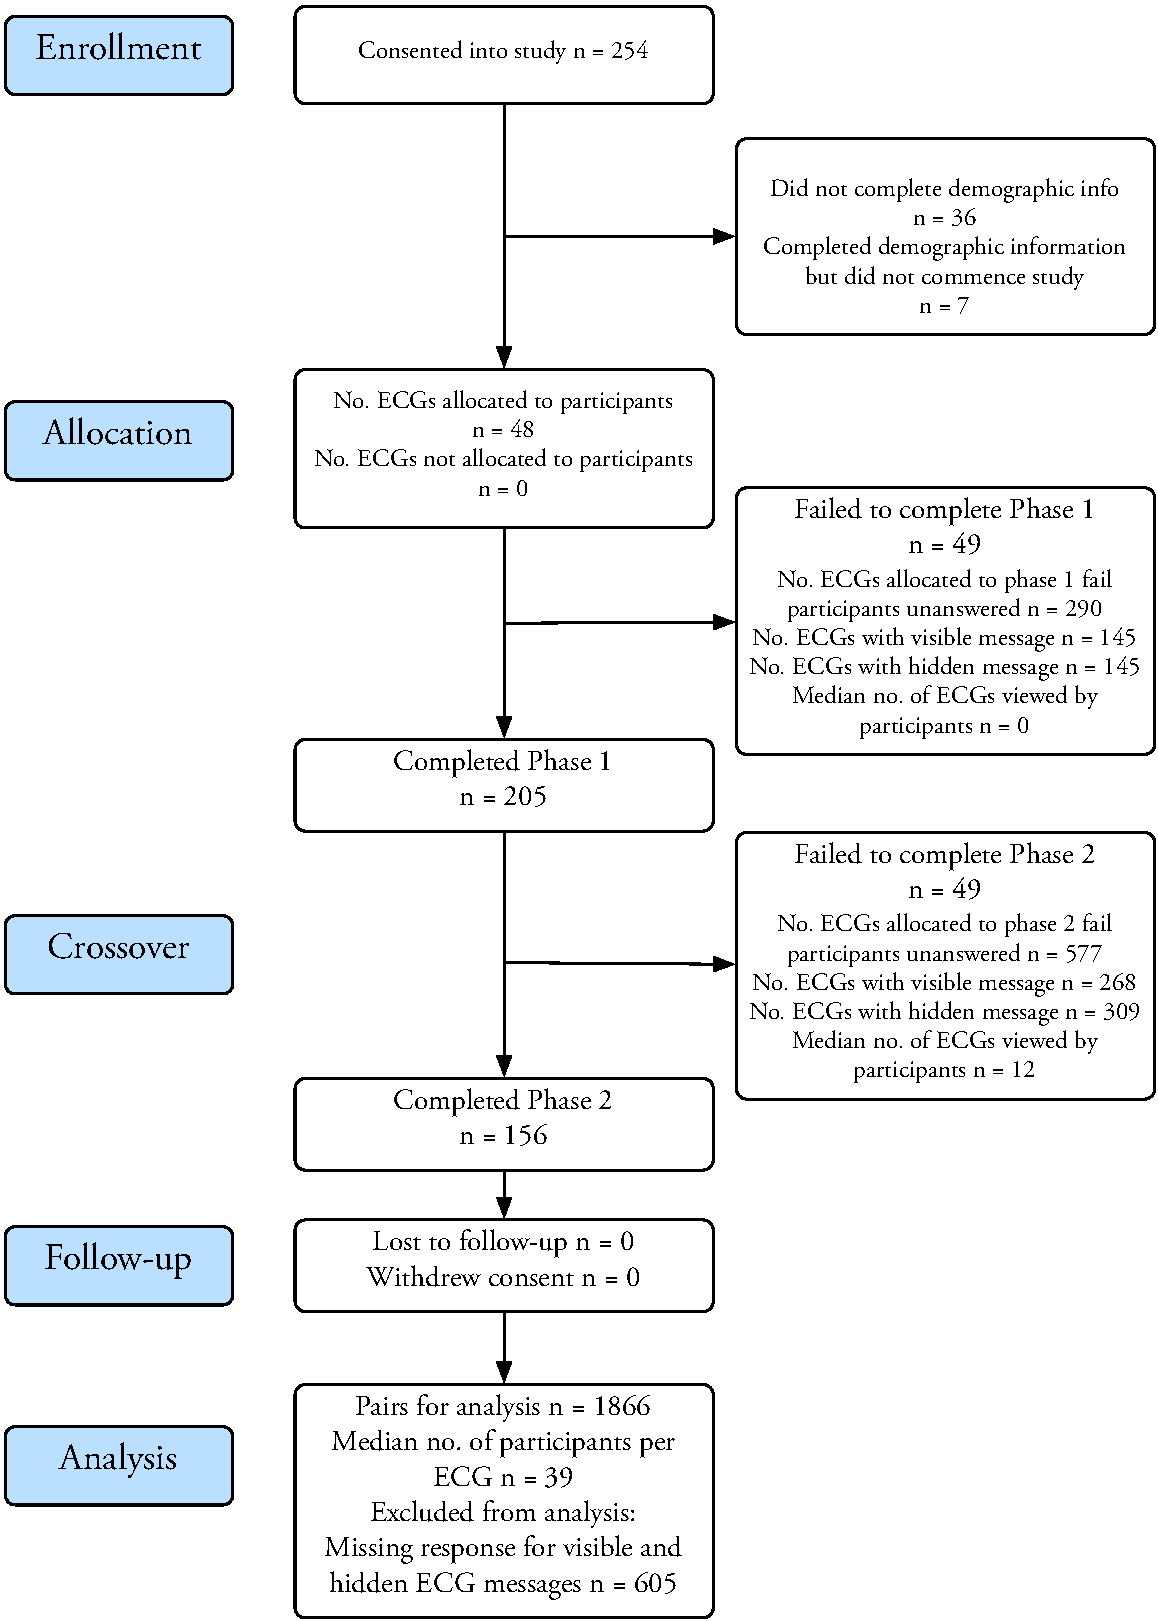
\includegraphics[keepaspectratio,width=\textwidth,height=0.9900\textheight,]{CONSORT-flow-diagram-pilot-completed.pdf}
\caption{CONSORT diagram for RESPECT pilot study}
\label{finalconsortpdf}
\end{figure}



 \newpage 

Demographic information was provided by 218 participants and this is summarised in \autoref{partcharfull}. There were 156 participants who completed both phases of the study and were included in the final analysis (\autoref{partcharfinish}), leaving 62 participants who did not complete the study (\autoref{partcharnofinish}). Aside from a lower median and interquartile range of CPD hours, they appear to have similar demographic characteristics. 

 % latex table generated in R 2.15.2 by xtable 1.7-1 package
% Mon Sep  2 18:40:13 2013
\begin{table}[htbp]
\centering
\caption{Summary of participant characteristics} 
\label{partcharfull}
\newcolumntype{K}{>{\centering\arraybackslash}p{0.13\textwidth}}
\newcolumntype{N}{>{\centering\arraybackslash}p{0.095\textwidth}}
\newcolumntype{B}{>{\arraybackslash}p{0.17\textwidth}}
\begin{tabular}{BKNNNNN}
  \hline
Characteristic & n & Lowest value & Lower quartile & Median & Upper quartile & Highest value \\ 
  \hline
Training route: &   &   &   &   &   &   \\ 
  Traditional & 134 (61\%) & - & - & - & - & - \\ 
  University & 84 (39\%) & - & - & - & - & - \\ 
  Service (yrs) & - & 0 & 2 & 5 & 10 & 32 \\ 
  CPD (hrs) & - & 0 & 1 & 4 & 10 & 160 \\ 
  pPCI patients & - & 0 & 2 & 4 & 6 & 41 \\ 
   \hline
\end{tabular}
\end{table}
 

 % latex table generated in R 2.15.2 by xtable 1.7-1 package
% Mon Sep  2 18:40:14 2013
\begin{table}[htbp]
\centering
\caption{Summary of participant characteristics who completed study} 
\label{partcharfinish}
\newcolumntype{K}{>{\centering\arraybackslash}p{0.13\textwidth}}
\newcolumntype{N}{>{\centering\arraybackslash}p{0.095\textwidth}}
\newcolumntype{B}{>{\arraybackslash}p{0.17\textwidth}}
\begin{tabular}{BKNNNNN}
  \hline
Characteristic & n & Lowest value & Lower quartile & Median & Upper quartile & Highest value \\ 
  \hline
Training route: &   &   &   &   &   &   \\ 
  Traditional & 96 (62\%) & - & - & - & - & - \\ 
  University & 60 (38\%) & - & - & - & - & - \\ 
  Service (yrs) & - & 0 & 2 & 5 & 10 & 32 \\ 
  CPD (hrs) & - & 0 & 2 & 5 & 11 & 160 \\ 
  pPCI patients & - & 0 & 1 & 3.5 & 5 & 41 \\ 
   \hline
\end{tabular}
\end{table}
 

 % latex table generated in R 2.15.2 by xtable 1.7-1 package
% Mon Sep  2 18:40:14 2013
\begin{table}[htbp]
\centering
\caption{Summary of participant characteristics who failed to complete study} 
\label{partcharnofinish}
\newcolumntype{K}{>{\centering\arraybackslash}p{0.13\textwidth}}
\newcolumntype{N}{>{\centering\arraybackslash}p{0.095\textwidth}}
\newcolumntype{B}{>{\arraybackslash}p{0.17\textwidth}}
\begin{tabular}{BKNNNNN}
  \hline
Characteristic & n & Lowest value & Lower quartile & Median & Upper quartile & Highest value \\ 
  \hline
Training route: &   &   &   &   &   &   \\ 
  Traditional & 38 (61\%) & - & - & - & - & - \\ 
  University & 24 (39\%) & - & - & - & - & - \\ 
  Service (yrs) & - & 0 & 2 & 5 & 10 & 30 \\ 
  CPD (hrs) & - & 0 & 0 & 2 & 6 & 120 \\ 
  pPCI patients & - & 0 & 3 & 4 & 6 & 30 \\ 
   \hline
\end{tabular}
\end{table}
 

\subsection{Incentives}
\label{incentives}

One of the aims of the pilot study was to examine the effect of incentives on attrition. To achieve this, participants were randomised into receiving one of the following incentive options:

\begin{itemize}
\item A CPD certificate

\item A prize draw for a paramedic textbook

\item Nothing.

\end{itemize}

\autoref{tableincentivefinal} shows the relation between randomised incentives and completion of the pilot study by participants. The chi-squared test for equality of proportions resulted in a p-value of 0.848, leading to the conclusion that there is no evidence that completion rates were dependent upon the incentive option.

\begin{table}[htbp]
\begin{minipage}{\linewidth}
\setlength{\tymax}{0.5\linewidth}
\centering
\small
\caption{Completion results by incentive offered}
\label{tableincentivefinal}
\begin{tabulary}{\textwidth}{@{}LLLL@{}} \toprule
&\multicolumn{2}{c}{Completed study}&\\
\textbf{Incentive}&\textbf{Yes}&\textbf{No}&\textbf{Total}\\
\midrule
Certificate&54 (74\%)&19 (26\%)&73\\
Prize draw&51 (71\%)&21(29\%)&72\\
None&51 (70\%)&22 (30\%)&73\\

\midrule
\textbf{Total}&156 (72\%)&62 (28\%)&218\\

\bottomrule

\end{tabulary}
\end{minipage}
\end{table}


\section{Electrocardiograms}
\label{electrocardiograms}

A complete set of summary statistics for each individual ECG, showing participant interpretation attempt and response times, can be found in \autoref{appendixh}. A concise synopsis of this data is shown in \autoref{meanpropecginteract}. 

 % latex table generated in R 2.15.2 by xtable 1.7-1 package
% Sat Aug 24 10:23:45 2013
\begin{table}[htbp]
\centering
\caption{Summary of participant interaction with ECGs} 
\label{meanpropecginteract}
\newcolumntype{D}{>{\arraybackslash}p{0.35\textwidth}}
                        \newcolumntype{E}{>{\centering\arraybackslash}p{0.1\textwidth}}
                        \newcolumntype{F}{>{\centering\arraybackslash}p{0.2\textwidth}}
                        \begin{tabular}{DEE|EE}
                       & \multicolumn{2}{F}{All data} & \multicolumn{2}{F}{Final data} \\
  \toprule
  & Median & Quartiles & Median & Quartiles \\ 
  \midrule
ECG interpretation attempts: total & 90 & 87-93 & 76 & 74-81 \\ 
  ECG interpretation attempts: message visible & 45 & 44-46 & 38 & 37-40 \\ 
  ECG interpretation attempts: message hidden & 44 & 42-46 & 38 & 37-41 \\ 
  Paired ECG interpretation attempts & 45 & 44-47 & 39 & 37-41 \\ 
   \bottomrule
\end{tabular}
\end{table}
 

The `All data' columns show the median and quartile values for an average ECG in the pilot study, when all ECG interpretation attempts are included. Final data, shows the same values, but only for the ECG interpretation attempts that were included in the final study analysis (i.e. after participants who had not completed both phases of the study were removed). There appears to be no evidence of differential completion rates between the message visibility of ECG interpretation attempts. A median of 39 paired ECG interpretation attempts for each ECG were available for the final analysis.

The boxplot figures (\autoref{boxplot1}, \autoref{boxplot2}, \autoref{boxplot3} and \autoref{boxplot4}) show the median ECG interpretation times by participant accuracy and computer interpretation for each ECG, sub-classified by message visibility. They demonstrate a wide range of ECG interpretation attempt completion times, suggesting that the time limit of 60 seconds, was appropriate.

 \begin{figure}[htbp]
\centerline{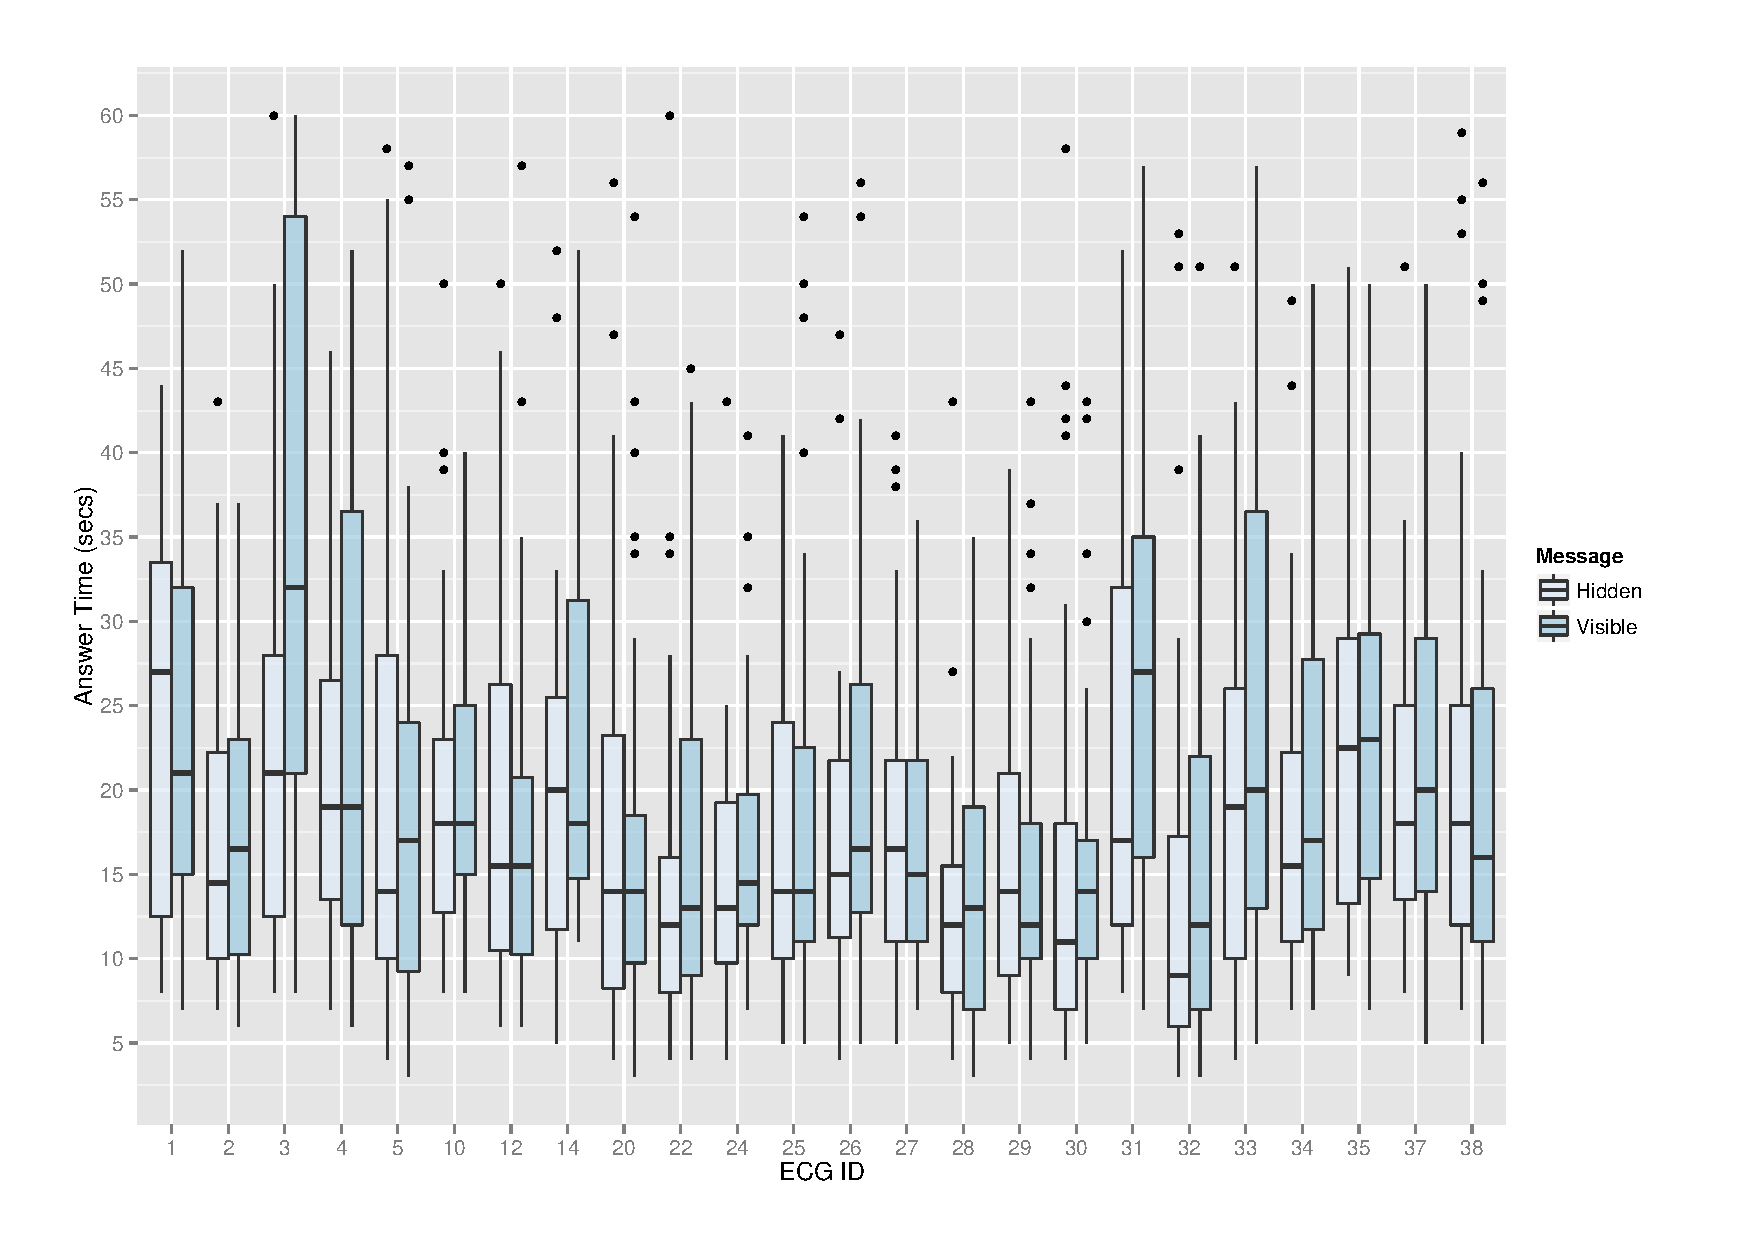
\includegraphics[page=1,keepaspectratio=false,width=0.8\paperwidth,height=0.45\paperwidth]{AnsTimeVsECG.pdf}}
\caption{Median answer time by ECG -- correct participant and computer interpretation}
\label{boxplot1}
\end{figure}

\begin{figure}[htbp]
\centerline{\includegraphics[page=2,keepaspectratio=false,width=0.8\paperwidth,height=0.45\paperwidth]{AnsTimeVsECG.pdf}}
\caption{Median answer time by ECG -- incorrect participant, and correct computer, interpretation}
\label{boxplot2}
\end{figure}

\begin{figure}[htbp]
\centerline{\includegraphics[page=3,keepaspectratio=false,width=0.8\paperwidth,height=0.45\paperwidth]{AnsTimeVsECG.pdf}}
\caption{Median answer time by ECG -- correct participant, and incorrect computer, interpretation}
\label{boxplot3}
\end{figure}

\begin{figure}[htbp]
\centerline{\includegraphics[page=4,keepaspectratio=false,width=0.8\paperwidth,height=0.45\paperwidth]{AnsTimeVsECG.pdf}}
\caption{Median answer time by ECG -- incorrect participant and computer interpretation}
\label{boxplot4}
\end{figure} 

 \newpage  

\section{Accuracy}
\label{accuracy}

\autoref{final2by2all} shows the sum totals of all responses by message visibility and answer accuracy. Participants in the pilot were correct approximately 80\% of the time, irrespective of whether the computer interpretation message was visible. 

\begin{table}[htbp]
\begin{minipage}{\linewidth}
\setlength{\tymax}{0.5\linewidth}
\centering
\small
\caption{Two-by-two table for all computer interpretations}
\label{final2by2all}
\begin{tabulary}{\textwidth}{@{}LCCC@{}} \toprule
&\multicolumn{2}{c}{Participant interpretation}&\\
Message&Correct&Incorrect&Total\\
\midrule
Visible&1481 (79\%)&385 (21\%)&1866\\
Hidden&1500 (80\%)&366 (20\%)&1866\\

\midrule
Total&2981(80\%)&751(20\%)&3732\\

\bottomrule

\end{tabulary}
\end{minipage}
\end{table}


When the data are split into correct and incorrect computer interpretations, a different pattern emerges. \autoref{final2by2correct} shows the results for ECGs with a correct computer interpretation. The results suggest that participants viewing this subset of ECGs, are more likely to make a correct interpretation. In addition, they are even more accurate when the computer interpretation message is visible.

\begin{table}[htbp]
\begin{minipage}{\linewidth}
\setlength{\tymax}{0.5\linewidth}
\centering
\small
\caption{Two-by-two table for all correct computer interpretations}
\label{final2by2correct}
\begin{tabulary}{\textwidth}{@{}LCCC@{}} \toprule
&\multicolumn{2}{c}{Participant interpretation}&\\
Message&Correct&Incorrect&Total\\
\midrule
Visible&816 (87\%)&117 (13\%)&933\\
Hidden&785 (84\%)&148 (16\%)&933\\

\midrule
Total&1601(86\%)&265 (14\%)&1866\\

\bottomrule

\end{tabulary}
\end{minipage}
\end{table}


Finally, \autoref{final2by2incorrect} shows the results for all ECGs with an incorrect computer interpretation. The results suggest that participants are less accurate in this sub-group, with 77\% of answers correct when the computer message is hidden, reducing to 71\% when the message is visible. 

\begin{table}[htbp]
\begin{minipage}{\linewidth}
\setlength{\tymax}{0.5\linewidth}
\centering
\small
\caption{Two-by-two table for all incorrect computer interpretations}
\label{final2by2incorrect}
\begin{tabulary}{\textwidth}{@{}LCCC@{}} \toprule
&\multicolumn{2}{c}{Participant interpretation}&\\
Message&Correct&Incorrect&Total\\
\midrule
Visible&665 (71\%)&268 (29\%)&933\\
Hidden&715 (77\%)&218 (23\%)&933\\

\midrule
Total&1380 (74\%)&486 (26\%)&1866\\

\bottomrule

\end{tabulary}
\end{minipage}
\end{table}


\section{Sensitivity and specificity}
\label{sensitivityandspecificity}

\autoref{partsensspec} shows the sensitivities and specificities for the participant responses, depending on computer interpretation accuracy and message visibility. There is little difference in sensitivity and specificity values, when participant ECG interpretation attempts of ECGs with correct and incorrect computer interpretation messages are analysed together.

  % latex table generated in R 2.15.2 by xtable 1.7-1 package
% Sun Aug 25 15:41:44 2013
\begin{table}[htbp]
\centering
\caption{Summary of sensitivities and specificities of participant responses} 
\label{partsensspec}
\newcolumntype{D}{>{\arraybackslash}p{0.3\textwidth}}
                        \newcolumntype{E}{>{\centering\arraybackslash}p{0.12\textwidth}}
                        \newcolumntype{F}{>{\centering\arraybackslash}p{0.24\textwidth}}
                        \begin{tabular}{DEE|EE}
                       & \multicolumn{2}{F}{Message Visible} & \multicolumn{2}{F}{Message Hidden} \\
  \toprule
Computer interpretation & Sensitivity & Specificity & Sensitivity & Specificity \\ 
  \midrule
All & 86 & 75 & 86 & 76 \\ 
  Correct & 92 & 85 & 89 & 80 \\ 
  Incorrect & 80 & 64 & 83 & 72 \\ 
   \bottomrule
\end{tabular}
\end{table}
  

However, if only the subgroup of participant interpretation attempts when the computer message is correct is considered, participants demonstrate a higher sensitivity and specificity, which increases further when the correct computer message is visible. Conversely, participant interpretation sensitivity and specificity decrease when only the ECGs which the computer interpreted incorrectly are included.

Overall, paramedics generally balance sensitivity and specificity quite well, with values around the 80\% mark, which is useful from a diagnostic perspective, but suggests that there is room for improvement. 

\section{Intra-class correlation coefficient}
\label{intra-classcorrelationcoefficient}

The intra-class correlation coefficient (ICC) is a measure of the degree of similarity between ECG interpretation attempts within a cluster. The ICC for participants is 0.05 and for ECGs, 0.41. The correlation between two randomly selected responses from the same participant, and the same ECG (known as the interaction ICC), was 0.46. These values suggest that taking clustering into account should make a significant difference in the GLM analysis.

\section{Generalised linear modelling results}
\label{generalisedlinearmodellingresults}

\autoref{ormesgall}, \autoref{ormesgcc} and \autoref{ormesgci} shows the results from the GLMs. The unadjusted odds ratios (OR) from the GLM are identical to those calculated from the two-by-two tables (\autoref{final2by2all}, \autoref{final2by2correct} and \autoref{final2by2incorrect}). Note that $ \sigma^2_{ecg}$ is the between-ECG variance for the random effects model and $ \sigma^2_{participant}$, the variance between participants. 

  % latex table generated in R 2.15.2 by xtable 1.7-1 package
% Sat Aug 24 13:35:11 2013
\begin{table}[htbp]
\centering
\caption{Odds ratio of correct interpretation} 
\label{ormesgall}
\begin{tabular}{lcccc}
  \toprule
Parameters & OR & z & P$>$$|z|$ & 95\% CI \\ 
  \midrule
\textit{Unadjusted for clustering}  &  &  &  & \\ 
  Constant & 4.10 & 24.20 & 0.00 & 3.66 to 4.60 \\ 
  Message & 0.94 & -0.78 & 0.44 & 0.80 to 1.10 \\ 
  \midrule
  \textit{Adjusted for clustering} &  &  &  & \\ 
  Constant & 6.48 & 9.42 & 0.00 & 4.39 to 9.56 \\ 
  Message & 0.92 & -0.88 & 0.38 & 0.77 to 1.10 \\ 
  \midrule 
  $\sigma^2_{ecg}$ & 1.57 &  &  &  \\ 
  $\sigma^2_{participant}$ & 0.21 &  &  &  \\ 
   \bottomrule
\end{tabular}
\end{table}
  

\autoref{ormesgcc} shows the odds ratio of a correct answer when the computer messages are correct. After adjusting for clustering, the odds ratio for the computer message has increased from 1.31 to 1.42. Conversely, in \autoref{ormesgci} it can be seen that the opposite result is obtained when the computer message is incorrect, as the odds ratio for the message decreases from 0.76 in the unadjusted model to 0.70 when clustering is taken into account.
  % latex table generated in R 2.15.2 by xtable 1.7-1 package
% Sat Aug 24 13:35:11 2013
\begin{table}[htbp]
\centering
\caption{Odds ratio of correct interpretation with correct computer message} 
\label{ormesgcc}
\begin{tabular}{lcccc}
  \toprule
Parameters & OR & z & P$>$$|z|$ & 95\% CI \\ 
  \midrule
\textit{Unadjusted for clustering}  &  &  &  & \\ 
  Constant & 5.30 & 18.62 & 0.00 & 4.46 to 6.35 \\ 
  Message & 1.31 & 2.05 & 0.04 & 1.01 to 1.71 \\ 
  \midrule
  \textit{Adjusted for clustering} &  &  &  & \\ 
  Constant & 9.16 & 8.32 & 0.00 & 5.43 to 15.43 \\ 
  Message & 1.42 & 2.36 & 0.02 & 1.06 to 1.89 \\ 
  \midrule 
  $\sigma^2_{ecg}$ & 1.57 &  &  &  \\ 
  $\sigma^2_{participant}$ & 0.21 &  &  &  \\ 
   \bottomrule
\end{tabular}
\end{table}
  

  % latex table generated in R 2.15.2 by xtable 1.7-1 package
% Sat Aug 24 13:35:12 2013
\begin{table}[htbp]
\centering
\caption{Odds ratio of correct interpretation with incorrect computer message} 
\label{ormesgci}
\begin{tabular}{lcccc}
  \toprule
Parameters & OR & z & P$>$$|z|$ & 95\% CI \\ 
  \midrule
\textit{Unadjusted for clustering}  &  &  &  & \\ 
  Constant & 3.28 & 15.35 & 0.00 & 2.82 to 3.82 \\ 
  Message & 0.76 & -2.63 & 0.01 & 0.61 to 0.93 \\ 
  \midrule
  \textit{Adjusted for clustering} &  &  &  & \\ 
  Constant & 4.95 & 5.80 & 0.00 & 2.88 to 8.49 \\ 
  Message & 0.70 & -3.03 & 0.00 & 0.56 to 0.88 \\ 
  \midrule 
  $\sigma^2_{ecg}$ & 1.57 &  &  &  \\ 
  $\sigma^2_{participant}$ & 0.21 &  &  &  \\ 
   \bottomrule
\end{tabular}
\end{table}
  

From the previous section, the ICC values suggested that the odds ratios would be significantly affected when clustering was taken into account. However, the odds ratios and confidence intervals from the GLM results do not appear to show this.
 % Results - 1149 words

\chapter{Discussion}
\label{discussion}

 \lhead{\emph{Discussion}} % Chapter title for thesis template 

\section{Summary of main findings}
\label{summaryofmainfindings}

The RESPECT pilot study has demonstrated that it is possible to conduct a randomised crossover trial to test the accuracy of STEMI recognition by paramedics, using an online assessment tool. The numbers of paramedics who participated in the pilot reflect the advantage of using an online, and access anywhere, method of delivering the assessment tool to maximise recruitment. Conducting this study using physical media would have been difficult to administrate, expensive and time consuming. However, despite the final number of participants being well in excess of the target of 50 for the pilot, almost 24\% of participants who completed phase 1, failed to return for phase 2 (the crossover). This is a potential threat to the validity of the study and also could have an impact on the target sample size for the main study. There was no evidence that the incentives offered in the pilot study made any difference to completion rates. However, it is possible that had they been advertised and\slash or offered together, that they may have been more effective.

Overall, participants were correct approximately 80\% of the time, irrespective of whether the computer message was visible (\autoref{final2by2all}). Participant sensitivity and specificity for all computer interpretations were almost identical, irrespective of whether the message was visible, or not, with a sensitivity of 86\% and specificity, 75--76\% depending on message visibility (\autoref{partsensspec}). This suggests that it is worth investigating ways to improve paramedics' recognition of STEMI.

The sub-group analysis does suggest that computer interpretation messages have an effect on participant interpretation, although this must be taken in the context of a non-powered pilot study. In the sub-group of ECGs where the computer interpretation was correct, the proportion of correct answers by participants when the message was hidden was 84\%, increasing to 87\% when the message was visible. Likewise, sensitivity and specificity increased when participants viewed the correct computer interpretation message. Conversely, in the sub-group of incorrect computer interpretation, the proportion of correct answers fell to 77\% with the message hidden, and to 71\% when the incorrect computer interpretation message was visible (\autoref{final2by2incorrect}). As before, sensitivity and specificity followed suit, with a reduction in both when the incorrect message was displayed. This suggests that both the computer and participant are more likely to correctly, and incorrectly, interpret similar types of ECGs, which is worth investigating in the main study.

Finally, the intra-class correlation coefficients (ICCs) will enable the calculation of the design effect of the main study. This is potentially the most serious threat to the feasibility of the main study, since if the sample size required to ensure the study is adequately powered is too large, then it would not be appropriate to proceed. The ICC for participants, was 0.05, which results in a design effect of 1.55, assuming a cluster size of 12 ECGs per participant. Of greater concern is the ICC for ECGs, which is 0.46. The median number of participants viewing each ECG in the pilot study, was 39, which would lead to a design effect of 18.48. Of course, these design effects are not separate, they both apply together and the calculation for an overall sample size for cross-classified models is non-trivial, may require Bayesian analysis~\citep{browne_comparison_2006} and will require expert statistical assistance.

The logistic regression analysis with random effects modelling appears to have been conducted accurately, having been confirmed in a separate statistics application. The scripts created for the pilot study (an example of which can be seen in \autoref{appendixi}), can be utilised for the main study and be modified as required.

Given the ICC values from the pilot study, it is reasonable to assume that larger standard errors and confidence intervals would have been seen when the unadjusted GLM was amended to account for clustering. However, the pilot data does not show this (\autoref{ormesgall}, \autoref{ormesgcc} and \autoref{ormesgci}) and this requires an explanation prior to commencing the main study. One possibility, is that the paired nature of the data has reduced the effect of the clustering of data. However, this needs to be reviewed by a statistician with an expertise in cluster randomised controlled trials. 

\section{Interpretation}
\label{interpretation}

Assuming that a satisfactory explanation can be obtained for the smaller than expected standard errors and confidence intervals, the rates of attrition can be addressed, and the required sample size to conduct the main study is not prohibitively large, the results from the pilot study are rather encouraging and support undertaking the main study. 

\section{Context}
\label{context}

The paramedic studies in the literature review (\autoref{literaturereview}) are difficult to compare directly with the RESPECT pilot since correctly excluded paramedic ECG interpretation attempts, and paramedic ECG interpretation without computer assistance, are not reported. \autoref{stemisubset} shows the proportions for the RESPECT pilot where the participants and the computer identified the ECG as a STEMI. This enables some form of comparison with the paramedic studies.

\begin{table}[htbp]
\begin{minipage}{\linewidth}
\setlength{\tymax}{0.5\linewidth}
\centering
\small
\caption{Two-by-two table showing data where computer and participant identified ECG as STEMI}
\label{stemisubset}
\begin{tabulary}{\textwidth}{@{}LCCC@{}} \toprule
&\multicolumn{2}{c}{STEMI present}&\\
Message&YES&NO&Total\\
\midrule
Visible&426 (72\%)&166 (28\%)&592\\
Hidden&412 (76\%)&138 (24\%)&550\\

\midrule
Total&838 (73\%)&304 (27\%)&1142\\

\bottomrule

\end{tabulary}
\end{minipage}
\end{table}


Paramedics appeared to perform slightly better in the Cantor study~\citep{cantor_prehospital_2012}, with paramedics correctly identifying STEMI in 106\slash 134 (79\%) of cases (assisted with computer interpretation) compared with 426\slash 592 (72\%) in the pilot study, although they would have had the benefit of the patient presentation and history to assist in their decision making. Paramedics in the Selker study~\citep{selker_emergency_2011} did not perform as well, despite having computer interpretation available, correctly recognising STEMI in 296\slash 437 (68\%) of patients. Finally, in the Ting study~\citep{ting_abstract_2009} paramedics performed much better, with 26\slash 30 (87\%) of patients correctly identified as STEMI by the paramedic (assisted by computer interpretation), although the sample size is small.

The doctor studies~\citep{goodacre_computer_2001,massel_observer_2003,tsai_computer_2003} are more aligned to the RESPECT pilot methodologically, allowing a more direct comparison of results. The participants in the Tsai study were not as accurate as the pilot participants, but there was similarity in the pattern of the results. In the sub-group of correct computer interpretations, participants in the Tsai study made a correct diagnosis in 255\slash 480 (53\%) of ECGs when the message was not visible, which rose to a statistically significant 327\slash 480 (68\%, p$<$0.001) when the message was visible. In contrast, when only ECGs with incorrect computer interpretations were considered, 102\slash 180 (57\%) were interpreted correctly, reducing to 87\slash 180 (48\%) when the incorrect computer interpretation was displayed (p=0.131). However, the Tsai study ECGs were not limited to STEMI and STEMI-mimics.

The Massel study showed a more modest change in the decision making of junior doctors when interpreting ECGs: when considering whether to administer thrombolysis, the participants were more likely to undercall a thrombolysis decision when the message was visible. However, further, more in-depth comparison with the pilot study is not possible based on the published results. The Goodacre study, similarly to the pilot study, found that overall the computer message did not significantly effect the junior doctors' decisions, but it was not limited to ECGs with STEMIs and STEMI-mimics, unlike the RESPECT pilot study.

\section{Strengths and limitations}
\label{strengthsandlimitations}

The use of a crossover design is powerful in terms of reducing between-subject variability, making crossover trials more efficient than a similar sized parallel group trial and, in theory, producing more precise estimates of treatment effects with the same sample size. A key drawback with crossover trials is the risk of `carry over', when the wash-out period is insufficient to allow the effects of the first treatment to wear off~\citep{mills_design_2009,sibbald_understanding_1998}. In this study the two week wash-out period was considered sufficient to ensure participants could not recall their first phase attempt, and the ECGs they viewed. However, a perceived poor performance in the first phase, may have prompted the participants to revise their knowledge on ECGs, and so be better prepared for the second phase, or not to return at all. However, the reason for not returning for the second phase was not recorded in the pilot study. Since approximately 24\% of participants failed the study, there is a risk of attrition bias, which may have been compounded by the removal of incomplete results for the final analysis. 

From the results of the incentive randomisation, it can be seen that there is no statistically significant difference in completion rates between the three incentive options. However, due to an inadvertent usability error, whereby the download link for the certificate did not automatically appear at the end of the study, a number of participants did contact the researcher asking for the certificate. A better advertised incentive at the start of the study, may assist in completion rates.

The website assessment tool performed well, and since the allocation of ECGs and their randomisation was handled automatically, no intervention was required by the researcher, thus minimising the risk of observer bias. In addition, the website handled the wash-out period, not allowing participants to undertake phase two until the allotted time had passed, and inviting them to return by email, as well as sending out periodic reminders. Due to the design, replicating the study is straightforward and can be customised as required (for example, if overseas paramedics take part in a subsequent study).

There was a risk that participants may have utilised textbooks or an expert colleague to assist with their answers, since the study is not supervised by the researcher. However, the time limited nature of the assessment (each ECG is only visible for 60 seconds) and the inability to view the same ECG with a specific message visibility (i.e. visible or hidden) more than once, should have minimised the chance of this happening.

Ultimately, this is an experiment, and a proxy for the interpretation of an ECG in the presence of an acutely ill patient. However, to replicate this study prospectively with genuine patient episodes would be complicated and expensive, and make extracting the role of the computer message alone from the other benefits of an actual patient encounter (such as patient presentation and history) difficult. In addition, this is a pilot with no \emph{a priori} power calculations and the results need to be confirmed by an adequately powered study.

\section{Implications for practice}
\label{implicationsforpractice}

The results from this pilot study should be interpreted with caution, and an adequately powered study is required before too much emphasis can be placed on the findings. The types of ECGs that the computer algorithms are more likely to misinterpret are known,~\citep{ting_implementation_2008} as are the modifiable factors that lead to error, such as incorrect lead placement~\citep{mccann_accuracy_2007,rajaganeshan_accuracy_2008}, incorrect identification of the J-point~\citep{williams_paramedic_2008} and even vehicular movement~\citep{hebel_accuracy_1994}. If it is the case that paramedics' diagnostic accuracy is being adversely affected by computer interpretation, then the education of paramedics in 12-lead ECG acquisition and interpretation would benefit from being reviewed to see whether this could be addressed.

Alternatively, the computer interpretation messages could be turned off. However, there is a risk that if this is undertaken, then correct interpretation by paramedics, based on the pilot study results, would decrease. The accuracy of computer interpretation varies from study to study, but false positive rates are around 22\% and false negative, 6--9\%~\citep{clark_automated_2010}. Paramedics' accuracy does appear to improve these rates, with false positive results ranging from 15--18\% and false negative, from 1--6\%~\citep{feldman_real-time_2005,trivedi_can_2009,le_may_citywide_2008}. However, a recent US, multi-EMS system study, used a survey tool on 477 paramedics and found that they were poor at spotting STEMI-mimics, correctly interpreting known STEMI-mimics such as left ventricular hypertrophy (LVH) and left bundle branch block (LBBB) less than 40\% of the time~\citep{mencl_paramedic_2013}. It is difficult to know how generalisable these results are to the UK, since little research has been conducted with UK paramedics in the past 10 years, which can provide an estimate of paramedics' accuracy in the recognition (or exclusion) of STEMI. 

\section{Future research}
\label{futureresearch}

These results need to be confirmed by an adequately powered study, assuming that the required sample size does not make the main study impracticable to conduct. It would also be helpful to conduct a qualitative study to explore how paramedics interpret 12-lead ECGs in the context of STEMI, and try to identify what role the computer interpretation message plays in their decision making. Utilising participants in the RESPECT study, who have consented to be contacted for subsequent research, would make it possible to identify a purposeful sample of participants for such a study, based on the influence that computer interpretation messages have on their decision about whether a STEMI is present or not.
 % Discussion - 2099 words

\chapter{Conclusion}
\label{conclusion}

 \lhead{\emph{Conclusion}} % Chapter title for thesis template 

The RESPECT pilot study has demonstrated that it is possible to conduct a randomised crossover trial to test the accuracy of STEMI recognition by paramedics, using an online assessment tool. The next step is to calculate the sample size for an adequately powered main study. If this is not prohibitively high, the main study should be conducted to see whether the results suggested from the pilot data can be replicated. The sample size calculation, confirmation of the appropriate model that should be utilised, and an explanation for the smaller than expected standard errors and confidence intervals for the adjusted GLM, will require the services of a statistician with an expertise in cluster randomised controlled trials.
 % Conclusion - 123 words

%% ----------------------------------------------------------------
% Now begin the Appendices, including them as separate files

\addtocontents{toc}{\vspace{2em}} % Add a gap in the Contents, for aesthetics

\appendix % Cue to tell LaTeX that the following 'chapters' are Appendices

%% Appendix A

\chapter{Summary of study ECGs}
\label{appendixa}
\lhead{Appendix A. \emph{Summary of study ECGs}}

\clearpage

\centering
 \renewcommand{\arraystretch}{2.0}
 \newcolumntype{L}{>{\raggedright\arraybackslash}p{0.1\textwidth}}
 \newcolumntype{A}{>{\raggedright\arraybackslash}p{0.25\textwidth}}
 \tiny
\begin{longtable}[c]{Lp{0.18\textwidth}AA}
\caption{Summary of study ECGs}\\
\hline
\textbf{ECG ID} & \textbf{Classification} & \textbf{Actual interpretation} & \textbf{Computer interpretation} \\
\hline
\endfirsthead
\multicolumn{4}{c}
{\tablename\ \thetable\ -- \textit{Continued from previous page}} \\
\hline
\textbf{ECG ID} & \textbf{Classification} & \textbf{Actual interpretation} & \textbf{Computer interpretation} \\
\hline
\endhead
\hline \multicolumn{4}{r}{\textit{Continued on next page}} \\
\endfoot
\hline
\endlastfoot
1&True negative&Early repolarisation&Otherwise normal ECG,  \newline  Sinus bradycardia, \newline  Early repolarisation \\
2&True negative&Normal sinus rhythm, \newline  Old inferior MI&Abnormal ECG, \newline  Sinus rhythm, \newline  Possible inferior infarct - age undetermined \\
3&True positive&Inferolateral MI&Acute MI suspected, \newline  Unusual P axis, \newline  Low voltage QRS \\
4&True negative&Early repolarisation&Normal ECG or non-specific anomalies \\
5&True negative&Paced rhythm&Abnormal ECG, \newline  Demand pacing, \newline  LVH with secondary repolarisation abnormality, \newline  Widespread ST-T abnormality may be due to hypertrophy and\slash or ischaemia \\
6&False positive&Meets voltage criteria for LVH&Abnormal ECG, \newline  Meets ST elevation MI criteria, \newline  Sinus rhythm, \newline  Inferior ST elevation, \newline  consider acute \\
7&False positive&IVCD&Abnormal ECG,  \newline  Meets ST elevation MI criteria,  \newline  Sinus rhythm with 1st degree A-V block,  \newline  Extensive infarct - possibly acute \\
8&False positive&Pericarditis&Extensive myocardial infarction \\
9&False positive&Pericarditis&Extensive myocardial infarction \\
10&True negative&LBBB&Abnormal ECG Unconfirmed,  \newline  Normal sinus rhythm,  \newline  Left bundle branch block \\
11&False positive&Inverted P waves in inferior leads,  \newline  PR depression&Acute MI suspected,  \newline  Unusual P axis and short PR,  \newline  probably junctional rhythm, \newline ST elevation consider inferior injury or acute infarct \\
12&True negative&Early repolarisation&Otherwise normal ECG, sinus bradycardia \\
13&False positive&Atrial flutter&Acute MI suspected,  \newline  Atrial flutter with 4:1 AV conduction, \newline  ST elevation consider inferior injury or acute infarct \\
14&True negative&NSR, bifascicular block&Abnormal ECG unconfirmed,  \newline  Normal sinus rhythm, Right bundle branch block,  \newline  Left anterior fascicular block, Bifascicular block \\
15&False positive&LBBB&Medium sized myocardial infarction,  \newline  consider urgen reperfusion therapy \\
16&False positive&Early repolarisation&Acute MI suspected,  \newline  Sinus bradycardia with sinus arrhythmia,  \newline  ST elevation consider anterolateral injury or acute infarct,  \newline  ST elevation consider inferior injury or acute infarct \\
17&False positive&Hyperkalaemia&Acute MI suspected, \newline  Atrial fibrillation with rapid ventricular response, \newline  Indeterminate axis,  \newline  Low voltage QRS,  \newline  ST elevation lateral injury or acute infarct \\
18&False positive&LVH, early repolarisation&Extensive myocardial infarction \\
19&False positive&Osborne waves&Meets ST elevation criteria,  \newline  Atrial fibrillation, \newline  Prolonged QT interval,  \newline  Widespread ST elevation,  \newline  consider acute infarct,  \newline  Anteroseptal ST depression is probably reciprocal to inferior infarct, \newline  ST junctional depression is non-specific \\
20&True negative&Paced rhythm&Abnormal ECG,  \newline  Normal sinus rhythm,  \newline  Ventricular pre-excitation,  \newline  WPW pattern type B \\
21&False negative&LAD occlusion, \newline  hyperacute T-waves&Abnormal ECG, sinus bradycardia,  \newline  moderate voltage criteria for LVH,  \newline  cannot rule out septal infarct, age undetermined \\
22&True positive&Anterolateral MI&Meets ST elevation MI criteria,  \newline  sinus rhythm, anteroseptal infarct - possibly acute,  \newline  lateral ST elevation,  \newline  consider acute infarct \\
23&False negative&Anterolateral MI&ECG override: data quality prohibits interpretation \\
24&True positive&Anterior MI&Meets ST elevation MI criteria,  \newline  sinus bradycardia, \newline  left axis deviation,  \newline  anteroseptal ST elevation, \newline  consider acute infarct,  \newline  inferior\slash lateral ST-T abnormality suggests myocardial injury\slash ischaemia \\
25&True positive&Anterolateral MI&Extensive myocardial infarction, consider urgent reperfusion therapy if patient's age $<$= 80 years \\
26&True positive&Inferolateral MI&Medium-sized myocardial infarction, consider urgent reperfusion therapy if the patient's age $<$= 70 years \\
27&True positive&Inferolateral MI&Extensive myocardial infarction, consider urgent reperfusion therapy if patient's age $<$= 80 years \\
28&True positive&Inferior MI&Meets ST elevation MI criteria, \newline  sinus rhythm, \newline  rightward axis, RVH with secondary repolarisation abnormality, \newline  inferior ST elevation consider acute infarct,  \newline  Ant\slash septal and lateral ST\_T abnormality \\
29&True positive&Anterolateral MI&Extensive myocardial infarction, consider urgent reperfusion therapy if patient's age $<$= 80 years \\
30&True positive&Anterior MI&Meets ST elevation MI criteria, \newline  sinus rhythm,  \newline  Lead(s) unsuitable for analysis: V4, IV conduction defect,  \newline  septal infarct - possibly acute,  \newline  inferior T wave abnormality is nonspecific \\
31&True negative&LBBB&Abnormal ECG unconfirmed,  \newline  Atrial fibrillation with PVCs,  \newline  QRS changes in V2 may be due to LVH but cannot rule out septal infarct,  \newline  Left ventricular hypertrophy,  \newline  inferio\slash lateral ST-T abnormality may be due to hypertrophy and\slash or ischaemia \\
32&True positive&Inferolateral MI&Extensive myocardial infarction, consider urgent reperfusion therapy if patient's age $<$= 80 years \\
33&True positive&Inferior MI&Extensive myocardial infarction, consider urgent reperfusion therapy if patient's age $<$= 80 years \\
34&True negative&Normal variant for age&Normal ECG of non-specific anomalies \\
35&True positive&Inferolateral MI&Meets ST elevation MI criteria,  \newline  atrial fibrillation with rapid ventricular response with PVCs or aberrant ventricular conduction,  \newline  inferior infarct - possibly acute, \newline  Lateral ST elevation consider acute infarct, Anteroseptal ST depression is probably \\
36&False negative&Inferior MI&ECG override: data quality prohibits interpretation \\
37&True negative&Meets voltage criteria for LVH&Abnormal ECG unconfirmed, sinus tachycardia,  \newline  Left ventricular hyptertrophy,  \newline  Anterolateral ST-T abnormality is probably due to ventricular hypertrophy \\
38&True negative&LBBB&Abnormal ECG unconfirmed \\
39&False negative&Anterior MI&Abnormal ECG unconfirmed,  \newline  Normal sinus rhythm,  \newline  Low voltage QRS,  \newline  Cannot rule out anteroseptal infarct age undetermined \\
40&False negative&Anterior MI&Abnormal ECG unconfirmed,  \newline  normal sinus rhythm, septal infarct age undetermined \\
41&False negative&Inferolateral MI&Abnormal ECG unconfirmed,  \newline  sinus bradycardia, \newline  ST elevation, consider early repolarisation, pericarditis, or injury,  \newline  ST abnormality, possible digitalis effect \\
42&False positive&Early repolarisation&Acute MI suspected,  \newline  abnormal ECG unconfirmed, \newline  sinus bradycardia with sinus arrhythmia, ST elevation consider anterolateral injury or acute infarct,  \newline  ST elevation consider inferior injury or acute infarct \\
43&False negative&Inferior MI&ECG override: data quality prohibits interpretation \\
44&False negative&Inferior MI&ECG override: data quality prohibits interpretation \\
45&False negative&Anterolateral MI&ECG override: data quality prohibits interpretation \\
46&False negative&Inferior MI&Abnormal ECG unconfirmed \\
47&False negative&Inferior MI&Abnormal ECG unconfirmed \\
48&False negative&Anterolateral MI&Abnormal ECG unconfirmed \\
\end{longtable}
 \renewcommand{\arraystretch}{1}
\normalsize	%Keyword search for lit review

% Appendix A

\chapter{Summary of study ECGs}
\label{appendixa}
\lhead{Appendix A. \emph{Summary of study ECGs}}

\clearpage

\centering
 \renewcommand{\arraystretch}{2.0}
 \newcolumntype{L}{>{\raggedright\arraybackslash}p{0.1\textwidth}}
 \newcolumntype{A}{>{\raggedright\arraybackslash}p{0.25\textwidth}}
 \tiny
\begin{longtable}[c]{Lp{0.18\textwidth}AA}
\caption{Summary of study ECGs}\\
\hline
\textbf{ECG ID} & \textbf{Classification} & \textbf{Actual interpretation} & \textbf{Computer interpretation} \\
\hline
\endfirsthead
\multicolumn{4}{c}
{\tablename\ \thetable\ -- \textit{Continued from previous page}} \\
\hline
\textbf{ECG ID} & \textbf{Classification} & \textbf{Actual interpretation} & \textbf{Computer interpretation} \\
\hline
\endhead
\hline \multicolumn{4}{r}{\textit{Continued on next page}} \\
\endfoot
\hline
\endlastfoot
1&True negative&Early repolarisation&Otherwise normal ECG,  \newline  Sinus bradycardia, \newline  Early repolarisation \\
2&True negative&Normal sinus rhythm, \newline  Old inferior MI&Abnormal ECG, \newline  Sinus rhythm, \newline  Possible inferior infarct - age undetermined \\
3&True positive&Inferolateral MI&Acute MI suspected, \newline  Unusual P axis, \newline  Low voltage QRS \\
4&True negative&Early repolarisation&Normal ECG or non-specific anomalies \\
5&True negative&Paced rhythm&Abnormal ECG, \newline  Demand pacing, \newline  LVH with secondary repolarisation abnormality, \newline  Widespread ST-T abnormality may be due to hypertrophy and\slash or ischaemia \\
6&False positive&Meets voltage criteria for LVH&Abnormal ECG, \newline  Meets ST elevation MI criteria, \newline  Sinus rhythm, \newline  Inferior ST elevation, \newline  consider acute \\
7&False positive&IVCD&Abnormal ECG,  \newline  Meets ST elevation MI criteria,  \newline  Sinus rhythm with 1st degree A-V block,  \newline  Extensive infarct - possibly acute \\
8&False positive&Pericarditis&Extensive myocardial infarction \\
9&False positive&Pericarditis&Extensive myocardial infarction \\
10&True negative&LBBB&Abnormal ECG Unconfirmed,  \newline  Normal sinus rhythm,  \newline  Left bundle branch block \\
11&False positive&Inverted P waves in inferior leads,  \newline  PR depression&Acute MI suspected,  \newline  Unusual P axis and short PR,  \newline  probably junctional rhythm, \newline ST elevation consider inferior injury or acute infarct \\
12&True negative&Early repolarisation&Otherwise normal ECG, sinus bradycardia \\
13&False positive&Atrial flutter&Acute MI suspected,  \newline  Atrial flutter with 4:1 AV conduction, \newline  ST elevation consider inferior injury or acute infarct \\
14&True negative&NSR, bifascicular block&Abnormal ECG unconfirmed,  \newline  Normal sinus rhythm, Right bundle branch block,  \newline  Left anterior fascicular block, Bifascicular block \\
15&False positive&LBBB&Medium sized myocardial infarction,  \newline  consider urgen reperfusion therapy \\
16&False positive&Early repolarisation&Acute MI suspected,  \newline  Sinus bradycardia with sinus arrhythmia,  \newline  ST elevation consider anterolateral injury or acute infarct,  \newline  ST elevation consider inferior injury or acute infarct \\
17&False positive&Hyperkalaemia&Acute MI suspected, \newline  Atrial fibrillation with rapid ventricular response, \newline  Indeterminate axis,  \newline  Low voltage QRS,  \newline  ST elevation lateral injury or acute infarct \\
18&False positive&LVH, early repolarisation&Extensive myocardial infarction \\
19&False positive&Osborne waves&Meets ST elevation criteria,  \newline  Atrial fibrillation, \newline  Prolonged QT interval,  \newline  Widespread ST elevation,  \newline  consider acute infarct,  \newline  Anteroseptal ST depression is probably reciprocal to inferior infarct, \newline  ST junctional depression is non-specific \\
20&True negative&Paced rhythm&Abnormal ECG,  \newline  Normal sinus rhythm,  \newline  Ventricular pre-excitation,  \newline  WPW pattern type B \\
21&False negative&LAD occlusion, \newline  hyperacute T-waves&Abnormal ECG, sinus bradycardia,  \newline  moderate voltage criteria for LVH,  \newline  cannot rule out septal infarct, age undetermined \\
22&True positive&Anterolateral MI&Meets ST elevation MI criteria,  \newline  sinus rhythm, anteroseptal infarct - possibly acute,  \newline  lateral ST elevation,  \newline  consider acute infarct \\
23&False negative&Anterolateral MI&ECG override: data quality prohibits interpretation \\
24&True positive&Anterior MI&Meets ST elevation MI criteria,  \newline  sinus bradycardia, \newline  left axis deviation,  \newline  anteroseptal ST elevation, \newline  consider acute infarct,  \newline  inferior\slash lateral ST-T abnormality suggests myocardial injury\slash ischaemia \\
25&True positive&Anterolateral MI&Extensive myocardial infarction, consider urgent reperfusion therapy if patient's age $<$= 80 years \\
26&True positive&Inferolateral MI&Medium-sized myocardial infarction, consider urgent reperfusion therapy if the patient's age $<$= 70 years \\
27&True positive&Inferolateral MI&Extensive myocardial infarction, consider urgent reperfusion therapy if patient's age $<$= 80 years \\
28&True positive&Inferior MI&Meets ST elevation MI criteria, \newline  sinus rhythm, \newline  rightward axis, RVH with secondary repolarisation abnormality, \newline  inferior ST elevation consider acute infarct,  \newline  Ant\slash septal and lateral ST\_T abnormality \\
29&True positive&Anterolateral MI&Extensive myocardial infarction, consider urgent reperfusion therapy if patient's age $<$= 80 years \\
30&True positive&Anterior MI&Meets ST elevation MI criteria, \newline  sinus rhythm,  \newline  Lead(s) unsuitable for analysis: V4, IV conduction defect,  \newline  septal infarct - possibly acute,  \newline  inferior T wave abnormality is nonspecific \\
31&True negative&LBBB&Abnormal ECG unconfirmed,  \newline  Atrial fibrillation with PVCs,  \newline  QRS changes in V2 may be due to LVH but cannot rule out septal infarct,  \newline  Left ventricular hypertrophy,  \newline  inferio\slash lateral ST-T abnormality may be due to hypertrophy and\slash or ischaemia \\
32&True positive&Inferolateral MI&Extensive myocardial infarction, consider urgent reperfusion therapy if patient's age $<$= 80 years \\
33&True positive&Inferior MI&Extensive myocardial infarction, consider urgent reperfusion therapy if patient's age $<$= 80 years \\
34&True negative&Normal variant for age&Normal ECG of non-specific anomalies \\
35&True positive&Inferolateral MI&Meets ST elevation MI criteria,  \newline  atrial fibrillation with rapid ventricular response with PVCs or aberrant ventricular conduction,  \newline  inferior infarct - possibly acute, \newline  Lateral ST elevation consider acute infarct, Anteroseptal ST depression is probably \\
36&False negative&Inferior MI&ECG override: data quality prohibits interpretation \\
37&True negative&Meets voltage criteria for LVH&Abnormal ECG unconfirmed, sinus tachycardia,  \newline  Left ventricular hyptertrophy,  \newline  Anterolateral ST-T abnormality is probably due to ventricular hypertrophy \\
38&True negative&LBBB&Abnormal ECG unconfirmed \\
39&False negative&Anterior MI&Abnormal ECG unconfirmed,  \newline  Normal sinus rhythm,  \newline  Low voltage QRS,  \newline  Cannot rule out anteroseptal infarct age undetermined \\
40&False negative&Anterior MI&Abnormal ECG unconfirmed,  \newline  normal sinus rhythm, septal infarct age undetermined \\
41&False negative&Inferolateral MI&Abnormal ECG unconfirmed,  \newline  sinus bradycardia, \newline  ST elevation, consider early repolarisation, pericarditis, or injury,  \newline  ST abnormality, possible digitalis effect \\
42&False positive&Early repolarisation&Acute MI suspected,  \newline  abnormal ECG unconfirmed, \newline  sinus bradycardia with sinus arrhythmia, ST elevation consider anterolateral injury or acute infarct,  \newline  ST elevation consider inferior injury or acute infarct \\
43&False negative&Inferior MI&ECG override: data quality prohibits interpretation \\
44&False negative&Inferior MI&ECG override: data quality prohibits interpretation \\
45&False negative&Anterolateral MI&ECG override: data quality prohibits interpretation \\
46&False negative&Inferior MI&Abnormal ECG unconfirmed \\
47&False negative&Inferior MI&Abnormal ECG unconfirmed \\
48&False negative&Anterolateral MI&Abnormal ECG unconfirmed \\
\end{longtable}
 \renewcommand{\arraystretch}{1}
\normalsize % Summary of ECGs

% Appendix B

\chapter{MLWin data analysis method}
\label{appendixb}
\lhead{Appendix B. \emph{MLWin data analysis method}}

\begin{figure}[htbp]
\centerline{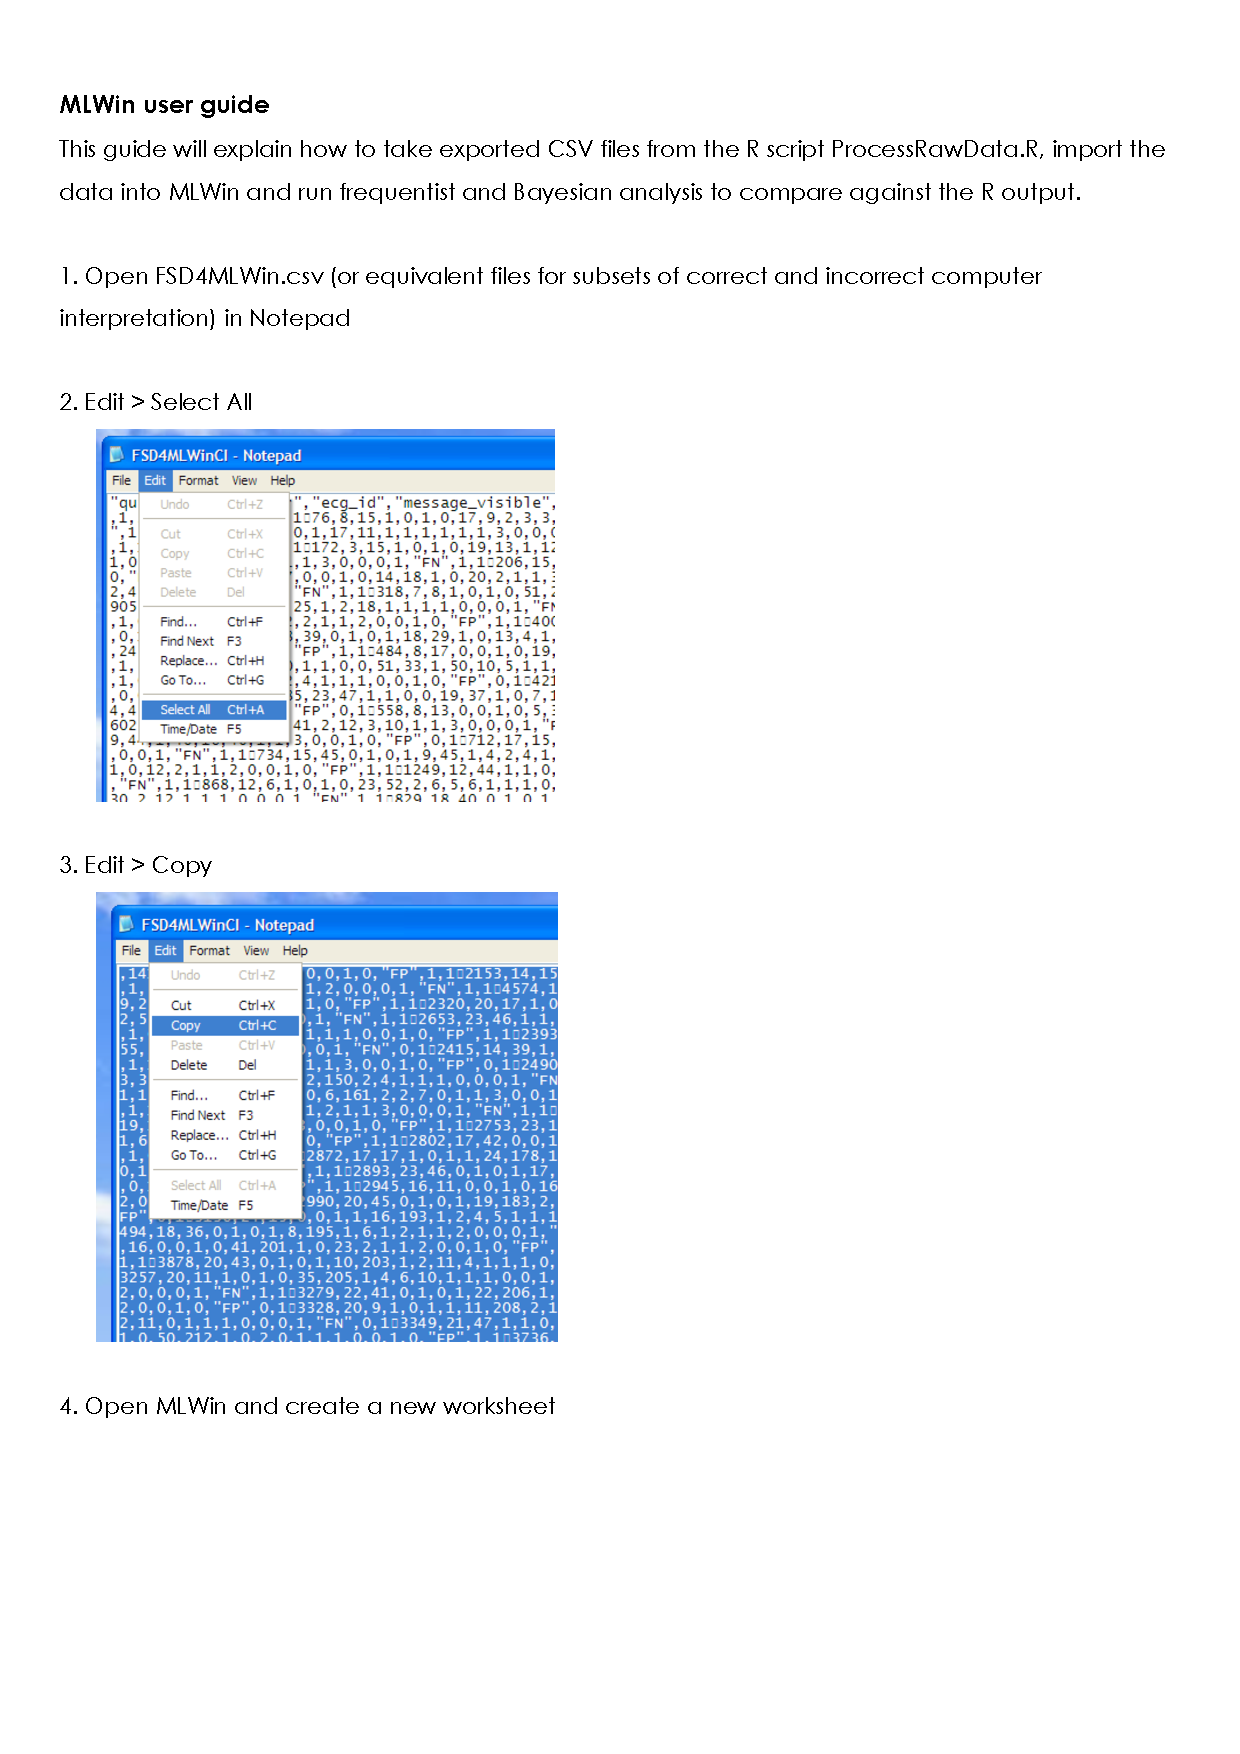
\includegraphics[page=1,keepaspectratio,width=0.9\paperwidth]{MLWin-respect.pdf}}
\label{partinfosheet1}
\end{figure}

\newpage

\begin{figure}[htbp]
\centerline{\includegraphics[page=2,keepaspectratio,width=0.9\paperwidth]{MLWin-respect.pdf}}
\label{partinfosheet2}
\end{figure}

\newpage

\begin{figure}[htbp]
\centerline{\includegraphics[page=3,keepaspectratio,width=0.9\paperwidth]{MLWin-respect.pdf}}
\label{partinfosheet3}
\end{figure}

\newpage

\begin{figure}[htbp]
\centerline{\includegraphics[page=4,keepaspectratio,width=0.9\paperwidth]{MLWin-respect.pdf}}
\label{partinfosheet4}
\end{figure}

\newpage

\begin{figure}[htbp]
\centerline{\includegraphics[page=5,keepaspectratio,width=0.9\paperwidth]{MLWin-respect.pdf}}
\label{partinfosheet5}
\end{figure}

\newpage

\begin{figure}[htbp]
\centerline{\includegraphics[page=6,keepaspectratio,width=0.9\paperwidth]{MLWin-respect.pdf}}
\label{partinfosheet6}
\end{figure}

\newpage

\begin{figure}[htbp]
\centerline{\includegraphics[page=7,keepaspectratio,width=0.9\paperwidth]{MLWin-respect.pdf}}
\label{partinfosheet7}
\end{figure}

\newpage

\begin{figure}[htbp]
\centerline{\includegraphics[page=8,keepaspectratio,width=0.9\paperwidth]{MLWin-respect.pdf}}
\label{partinfosheet8}
\end{figure}

\newpage

\begin{figure}[htbp]
\centerline{\includegraphics[page=9,keepaspectratio,width=0.9\paperwidth]{MLWin-respect.pdf}}
\label{partinfosheet9}
\end{figure}

\newpage

\begin{figure}[htbp]
\centerline{\includegraphics[page=10,keepaspectratio,width=0.9\paperwidth]{MLWin-respect.pdf}}
\label{partinfosheet10}
\end{figure}

\newpage

\begin{figure}[htbp]
\centerline{\includegraphics[page=11,keepaspectratio,width=0.9\paperwidth]{MLWin-respect.pdf}}
\label{partinfosheet11}
\end{figure}

\newpage

\begin{figure}[htbp]
\centerline{\includegraphics[page=12,keepaspectratio,width=0.9\paperwidth]{MLWin-respect.pdf}}
\label{partinfosheet12}
\end{figure}

\newpage

\begin{figure}[htbp]
\centerline{\includegraphics[page=13,keepaspectratio,width=0.9\paperwidth]{MLWin-respect.pdf}}
\label{partinfosheet13}
\end{figure}

\newpage

\begin{figure}[htbp]
\centerline{\includegraphics[page=14,keepaspectratio,width=0.9\paperwidth]{MLWin-respect.pdf}}
\label{partinfosheet14}
\end{figure}  % MLWin data testing method

% Appendix C

\chapter{YAS research and development approval}
\label{appendixc}
\lhead{Appendix C. \emph{YAS research and development approval}}

\begin{figure}[htbp]
\centerline{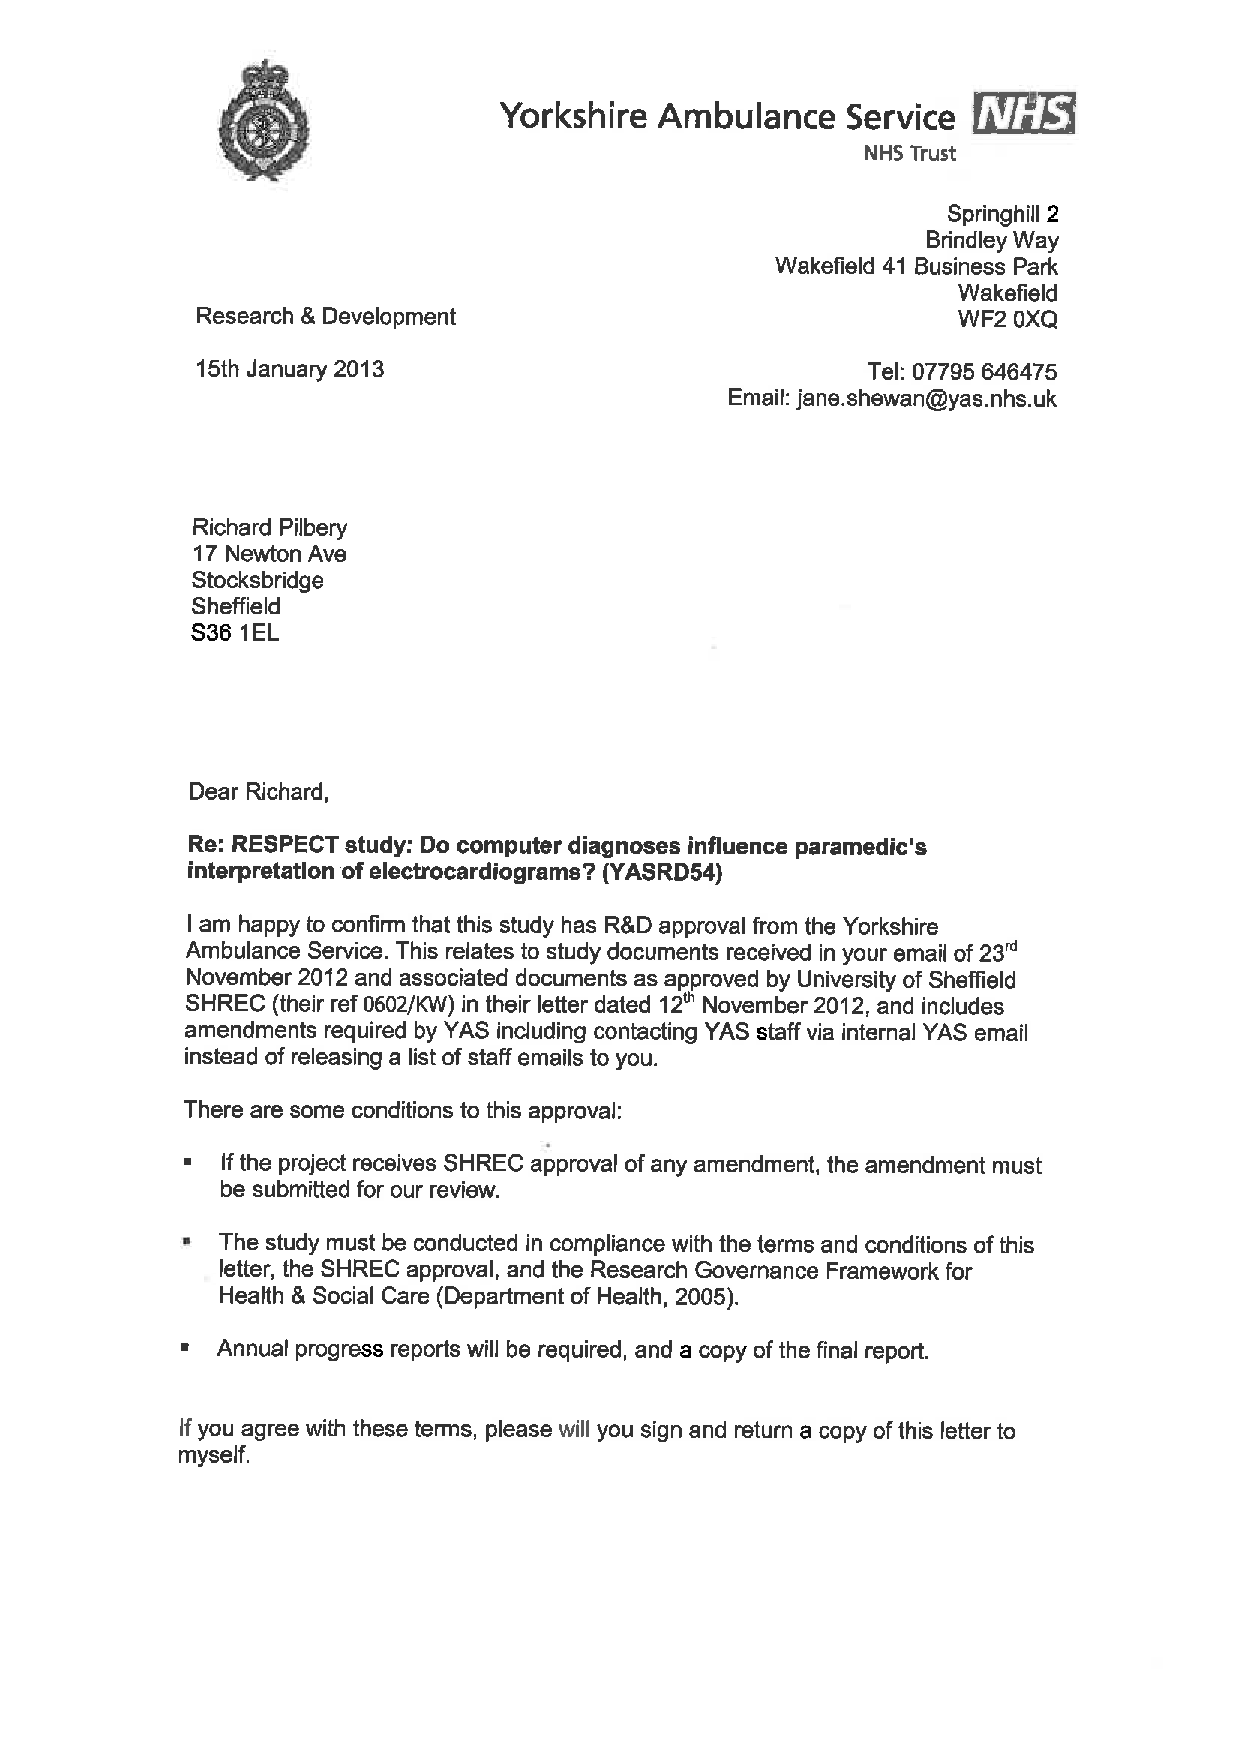
\includegraphics[page=1,keepaspectratio,width=0.9\paperwidth]{YASapprovalletterRPdissertation15thJan2013.pdf}}
\label{yasrdform1}
\end{figure}

\newpage

\begin{figure}[htbp]
\centerline{\includegraphics[page=2,keepaspectratio,width=0.9\paperwidth]{YASapprovalletterRPdissertation15thJan2013.pdf}}
\label{yasrdform2}
\end{figure} % YAS R&D approval

% Appendix D

\chapter{University ethics approval}
\label{appendixd}
\lhead{Appendix D. \emph{University ethics approval}}

\begin{figure}[htbp]
\centerline{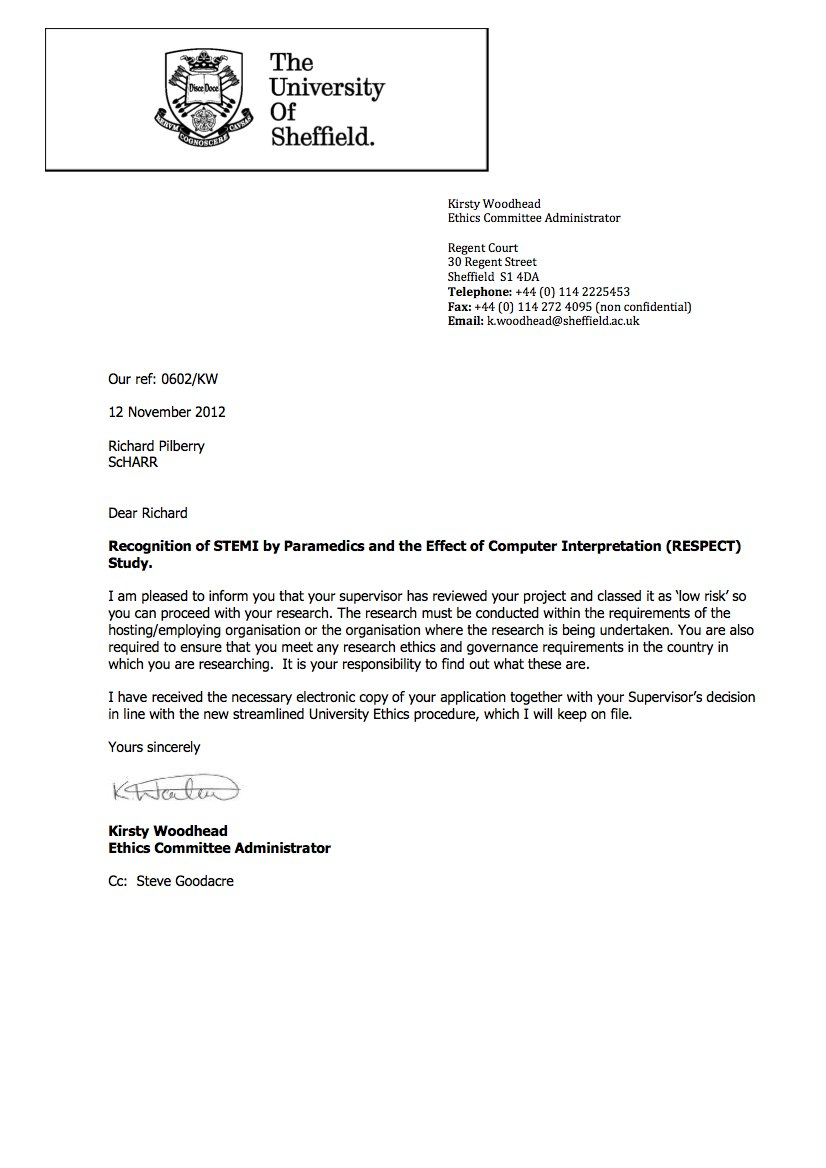
\includegraphics[page=1,keepaspectratio,width=0.8\paperwidth]{Approvalletter0602.jpg}}
\label{ethicsform}
\end{figure}
  % uni ethics

% Appendix E

\chapter{Research governance sponsorship confirmation}
\label{appendixe}
\lhead{Appendix E. \emph{Research governance sponsorship confirmation}}

\begin{figure}[htbp]
\centerline{
\includegraphics[page=1,keepaspectratio,width=0.8\paperwidth]{uni-sponsor.png}}
\label{sponsform}
\end{figure}
 % uni research sponsors confirmation

% Appendix F

\chapter{Risk assessment form}
\label{appendixf}
\lhead{Appendix F. \emph{Risk assessment form}}

\begin{figure}[htbp]
\centerline{
\includegraphics[page=1,keepaspectratio,width=0.8\paperwidth]{risk-assess1.jpg}}
\label{riskform1}
\end{figure}

\newpage

\begin{figure}[htbp]
\centerline{
\includegraphics[page=1,keepaspectratio,width=0.8\paperwidth]{risk-assess2.jpg}}
\label{riskform2}
\end{figure} % uni Risk assessment form

% Appendix G

\chapter{Participant information sheet}
\label{appendixg}
\lhead{Appendix G. \emph{Participant information sheet}}

\begin{figure}[htbp]
\centerline{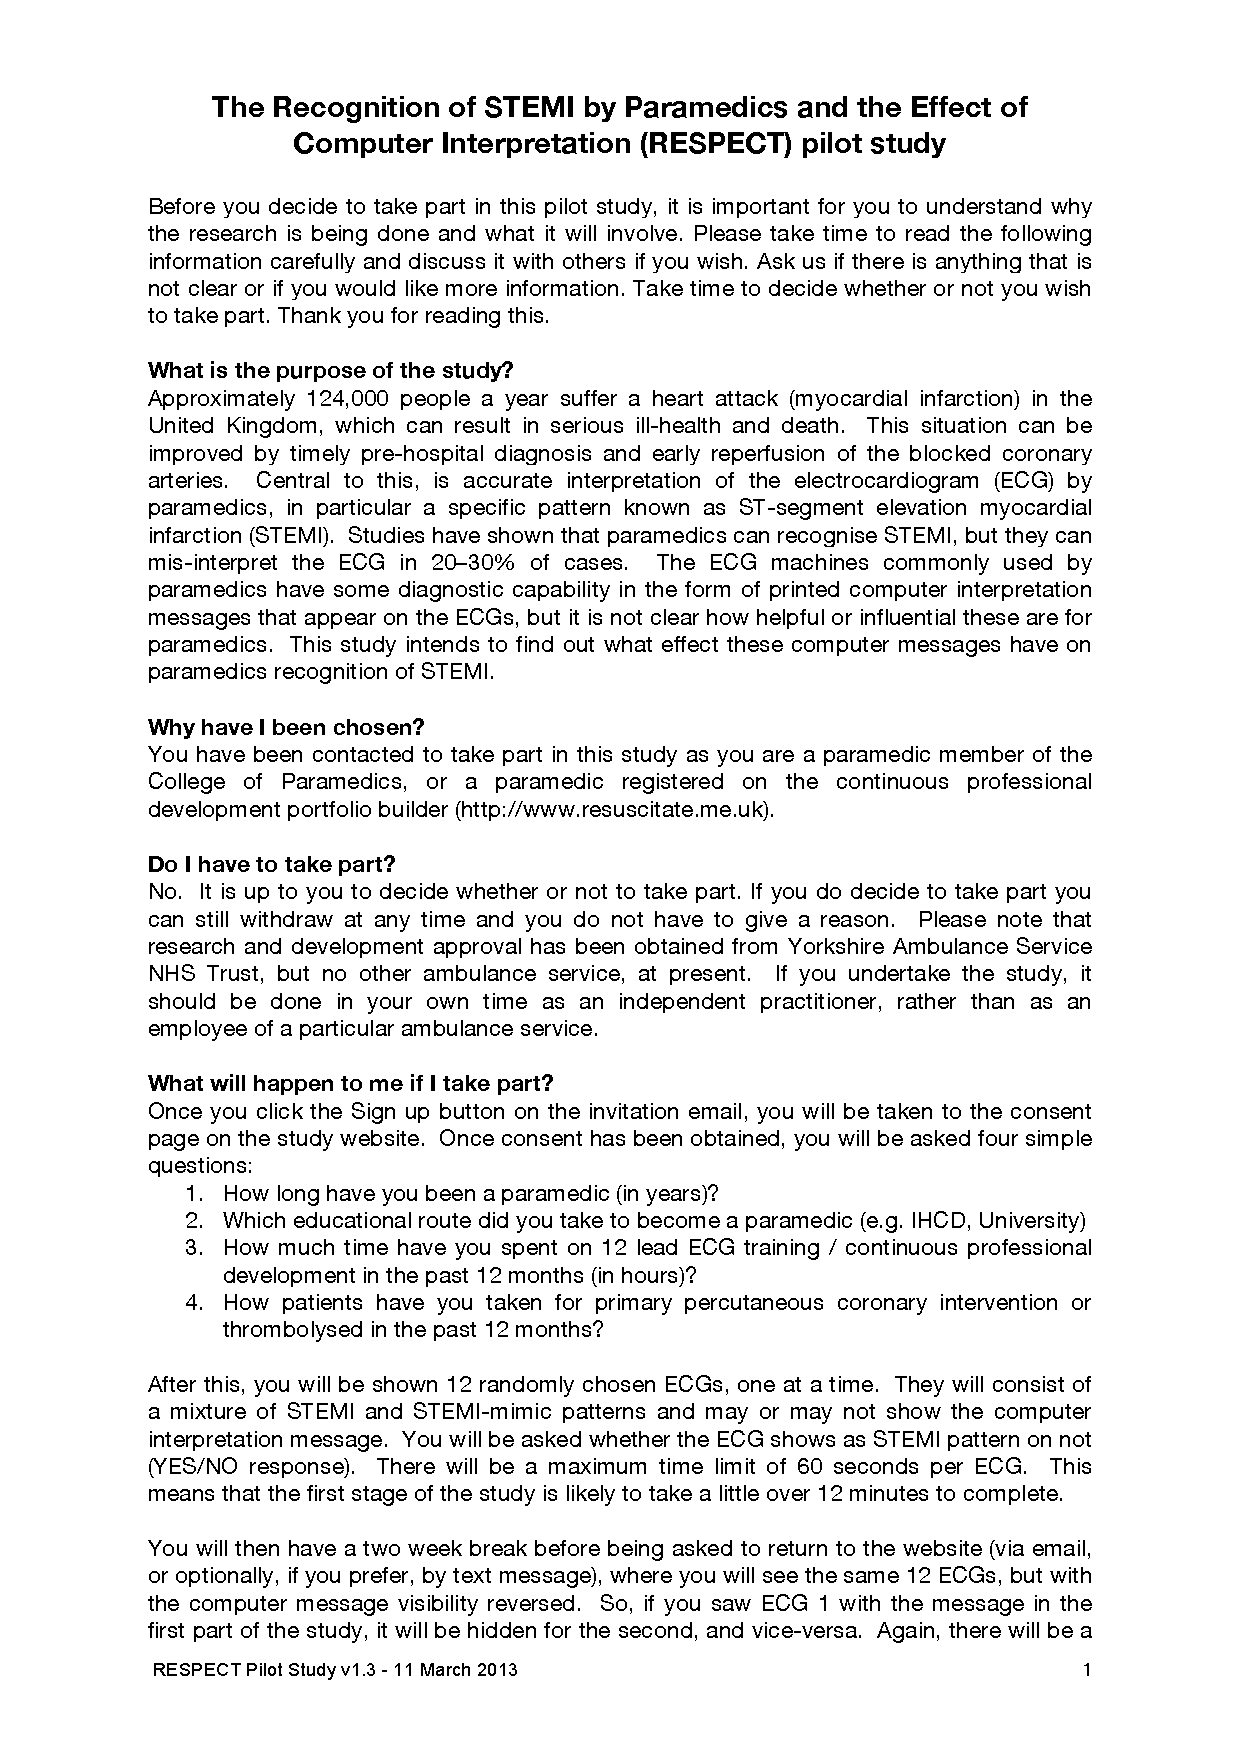
\includegraphics[page=1,keepaspectratio,width=0.8\paperwidth]{part-info-sheet.pdf}}
\label{partinfosheet1}
\end{figure}

\newpage

\begin{figure}[htbp]
\centerline{\includegraphics[page=2,keepaspectratio,width=0.8\paperwidth]{part-info-sheet.pdf}}
\label{partinfosheet2}
\end{figure}
 % Participant Information Sheet

% Appendix H

\chapter{Summary tables of participant responses to individual ECGs}
\label{appendixh}
\lhead{Appendix H. \emph{Summary tables of participant responses to individual ECGs}}

\begin{quote}
Key:\\
V message visible\\
H message hidden\\
T All messages\\
Data pairs - Paired responses with an answer for message visible and hidden for a single ECG and single participant\\
Excl. Orphaned data (ie missing one of message visible or hidden for a single ECG and single participant). This response will be deleted from the data set. 
\end{quote}

% This is the wrapper for partsumecginteract-middle.tex
% That file only contains the rows, so need to create the table wrapper around it

\begin{table}[htbp]
\begin{minipage}{\linewidth}
\setlength{\tymax}{0.5\linewidth}
\centering
\small
\caption{Summary of participant interaction with ECGs}
\label{partsumecginteract}
 \newcolumntype{G}{>{\centering\arraybackslash}p{0.035\textwidth}}
 \newcolumntype{H}{>{\centering\arraybackslash}p{0.06\textwidth}}
 \newcolumntype{J}{>{\centering\arraybackslash}p{0.2\textwidth}}
\begin{tabulary}{\textwidth}{@{}HGGGHGGGGGGH@{}} \toprule

\textbf{ECG ID}&\multicolumn{3}{J}{\textbf{Attempts with answer}}&\textbf{Data pairs}&\multicolumn{3}{J}
{\textbf{Not attempted}}&\multicolumn{3}{J}{\textbf{Unviewed}}&\textbf{Excl.}\\
&V&H&T&&V&H&T&V&H&T&\\
\midrule
% latex table generated in R 2.15.2 by xtable 1.7-1 package
% Sat Aug 24 10:36:05 2013
1 & 45 & 46 & 91 & 46 & 0 & 0 & 0 & 9 & 8 & 17 & 11 \\ 
  2 & 49 & 44 & 93 & 44 & 1 & 0 & 1 & 4 & 10 & 14 & 12 \\ 
  3 & 44 & 44 & 88 & 45 & 1 & 1 & 2 & 10 & 10 & 20 & 12 \\ 
  4 & 45 & 48 & 93 & 48 & 0 & 0 & 0 & 10 & 7 & 17 & 7 \\ 
  5 & 45 & 43 & 88 & 45 & 1 & 2 & 3 & 8 & 9 & 17 & 9 \\ 
  6 & 48 & 48 & 96 & 48 & 1 & 0 & 1 & 5 & 6 & 11 & 7 \\ 
  7 & 45 & 44 & 89 & 44 & 0 & 0 & 0 & 9 & 10 & 19 & 13 \\ 
  8 & 49 & 45 & 94 & 46 & 1 & 1 & 2 & 4 & 8 & 12 & 10 \\ 
  9 & 48 & 42 & 90 & 44 & 0 & 2 & 2 & 6 & 10 & 16 & 14 \\ 
  10 & 44 & 44 & 88 & 45 & 1 & 1 & 2 & 10 & 10 & 20 & 14 \\ 
  11 & 42 & 44 & 86 & 44 & 0 & 0 & 0 & 13 & 11 & 24 & 14 \\ 
  12 & 42 & 45 & 87 & 47 & 0 & 2 & 2 & 13 & 8 & 21 & 15 \\ 
  13 & 44 & 41 & 85 & 41 & 1 & 0 & 1 & 9 & 13 & 22 & 16 \\ 
  14 & 44 & 45 & 89 & 45 & 3 & 0 & 3 & 8 & 10 & 18 & 14 \\ 
  15 & 44 & 42 & 86 & 45 & 1 & 3 & 4 & 10 & 10 & 20 & 16 \\ 
  16 & 45 & 48 & 93 & 48 & 1 & 0 & 1 & 8 & 6 & 14 & 10 \\ 
  17 & 43 & 43 & 86 & 44 & 2 & 1 & 3 & 10 & 11 & 21 & 11 \\ 
  18 & 46 & 42 & 88 & 42 & 0 & 0 & 0 & 9 & 13 & 22 & 12 \\ 
  19 & 48 & 40 & 88 & 40 & 1 & 0 & 1 & 6 & 15 & 21 & 15 \\ 
  20 & 43 & 48 & 91 & 48 & 0 & 0 & 0 & 11 & 6 & 17 & 15 \\ 
  21 & 42 & 49 & 91 & 49 & 1 & 0 & 1 & 12 & 6 & 18 & 12 \\ 
  22 & 48 & 48 & 96 & 49 & 1 & 1 & 2 & 5 & 5 & 10 & 8 \\ 
  23 & 46 & 46 & 92 & 46 & 1 & 0 & 1 & 7 & 8 & 15 & 13 \\ 
  24 & 47 & 41 & 88 & 41 & 0 & 0 & 0 & 7 & 13 & 20 & 16 \\ 
  25 & 45 & 41 & 86 & 42 & 0 & 1 & 1 & 9 & 13 & 22 & 16 \\ 
  26 & 47 & 48 & 95 & 48 & 1 & 0 & 1 & 7 & 7 & 14 & 8 \\ 
  27 & 45 & 48 & 93 & 48 & 0 & 0 & 0 & 9 & 6 & 15 & 11 \\ 
  28 & 44 & 45 & 89 & 47 & 0 & 1 & 1 & 11 & 8 & 19 & 13 \\ 
  29 & 46 & 42 & 88 & 42 & 0 & 0 & 0 & 8 & 12 & 20 & 10 \\ 
  30 & 45 & 46 & 91 & 46 & 0 & 0 & 0 & 9 & 8 & 17 & 11 \\ 
  31 & 46 & 47 & 93 & 47 & 1 & 0 & 1 & 8 & 8 & 16 & 10 \\ 
  32 & 46 & 47 & 93 & 47 & 1 & 0 & 1 & 7 & 7 & 14 & 12 \\ 
  33 & 42 & 40 & 82 & 42 & 0 & 2 & 2 & 13 & 13 & 26 & 18 \\ 
  34 & 45 & 46 & 91 & 47 & 0 & 1 & 1 & 9 & 7 & 16 & 12 \\ 
  35 & 45 & 45 & 90 & 45 & 0 & 0 & 0 & 10 & 10 & 20 & 14 \\ 
  36 & 43 & 44 & 87 & 44 & 2 & 0 & 2 & 10 & 11 & 21 & 15 \\ 
  37 & 46 & 44 & 90 & 44 & 0 & 0 & 0 & 9 & 11 & 20 & 16 \\ 
  38 & 39 & 41 & 80 & 41 & 1 & 0 & 1 & 14 & 13 & 27 & 17 \\ 
  39 & 46 & 48 & 94 & 48 & 1 & 0 & 1 & 8 & 7 & 15 & 11 \\ 
  40 & 39 & 43 & 82 & 43 & 1 & 0 & 1 & 14 & 11 & 25 & 15 \\ 
  41 & 43 & 37 & 80 & 39 & 1 & 2 & 3 & 10 & 15 & 25 & 13 \\ 
  42 & 50 & 45 & 95 & 45 & 0 & 0 & 0 & 5 & 10 & 15 & 13 \\ 
  43 & 43 & 44 & 87 & 45 & 1 & 1 & 2 & 10 & 9 & 19 & 13 \\ 
  44 & 46 & 49 & 95 & 49 & 0 & 0 & 0 & 8 & 5 & 13 & 11 \\ 
  45 & 49 & 43 & 92 & 44 & 0 & 1 & 1 & 6 & 11 & 17 & 11 \\ 
  46 & 49 & 46 & 95 & 46 & 1 & 0 & 1 & 5 & 9 & 14 & 10 \\ 
  47 & 44 & 43 & 87 & 46 & 0 & 3 & 3 & 10 & 8 & 18 & 16 \\ 
  48 & 48 & 40 & 88 & 42 & 1 & 2 & 3 & 6 & 13 & 19 & 13 \\ 
   \bottomrule

\bottomrule

\end{tabulary}
\end{minipage}
\end{table} 

\begin{table}[htbp]
\begin{minipage}{\linewidth}
\setlength{\tymax}{0.5\linewidth}
\centering
\small
\caption{Summary of individual ECG answer times}
\label{ecgtimes}
 \newcolumntype{K}{>{\centering\arraybackslash}p{0.035\textwidth}}
 \newcolumntype{N}{>{\centering\arraybackslash}p{0.06\textwidth}}
 \newcolumntype{A}{>{\centering\arraybackslash}p{0.2\textwidth}}
\begin{tabulary}{\textwidth}{@{}NKKKKKKKKKKKK@{}} \toprule
\textbf{ECG ID}&\multicolumn{3}{A}{\textbf{Median correct answer time (secs)}}&\multicolumn{3}{A}{\textbf{Median incorrect answer time (secs)}}&\multicolumn{3}{A}{\textbf{No. Correct answers}}&\multicolumn{3}{A}{\textbf{No. Incorrect answers}}\\
&V&H&T&V&H&T&V&H&T&V&H&T\\
\midrule
% latex table generated in R 2.15.2 by xtable 1.7-1 package
1 & 24 & 27 & 26 & 20 & 27 & 27 & 38 & 26 & 64 & 7 & 20 & 27 \\ 
  2 & 17 & 14 & 16 & 42 & 27 & 33 & 45 & 38 & 83 & 5 & 6 & 11 \\ 
  3 & 32 & 23 & 29 & 22 & 17 & 18 & 17 & 14 & 31 & 28 & 31 & 59 \\ 
  4 & 20 & 19 & 19 & 30 & 24 & 24 & 32 & 29 & 61 & 13 & 19 & 32 \\ 
  5 & 18 & 14 & 17 & 32 & 45 & 39 & 35 & 39 & 74 & 11 & 6 & 17 \\ 
  6 & 18 & 12 & 16 & 25 & 5 & 20 & 46 & 47 & 93 & 3 & 1 & 4 \\ 
  7 & 28 & 22 & 23 & 25 & 27 & 26 & 30 & 29 & 59 & 15 & 15 & 30 \\ 
  8 & 32 & 28 & 30 & 20 & 26 & 26 & 25 & 27 & 52 & 25 & 19 & 44 \\ 
  9 & 26 & 20 & 22 & 25 & 21 & 24 & 31 & 33 & 64 & 17 & 11 & 28 \\ 
  10 & 20 & 18 & 18 & 28 & 28 & 28 & 40 & 34 & 74 & 5 & 11 & 16 \\ 
  11 & 22 & 19 & 20 & 39 & 32 & 35 & 36 & 39 & 75 & 6 & 5 & 11 \\ 
  12 & 16 & 16 & 16 & 28 & 25 & 26 & 34 & 42 & 76 & 8 & 5 & 13 \\ 
  13 & 18 & 14 & 15 & 29 &  & 29 & 42 & 41 & 83 & 3 & 0 & 3 \\ 
  14 & 18 & 20 & 20 & 20 & 24 & 20 & 31 & 33 & 64 & 16 & 12 & 28 \\ 
  15 & 20 & 15 & 17 & 25 & 25 & 25 & 24 & 25 & 49 & 21 & 20 & 41 \\ 
  16 & 30 & 26 & 27 & 18 & 16 & 17 & 22 & 28 & 50 & 24 & 20 & 44 \\ 
  17 & 18 & 14 & 17 & 17 & 30 & 17 & 39 & 38 & 77 & 6 & 6 & 12 \\ 
  18 & 27 & 18 & 23 & 30 & 24 & 28 & 28 & 30 & 58 & 18 & 12 & 30 \\ 
  19 & 32 & 18 & 24 & 20 & 20 & 20 & 19 & 15 & 34 & 30 & 25 & 55 \\ 
  20 & 13 & 14 & 14 & 19 & 16 & 16 & 41 & 44 & 85 & 2 & 4 & 6 \\ 
  21 & 38 & 28 & 32 & 22 & 23 & 23 & 17 & 20 & 37 & 26 & 29 & 55 \\ 
  22 & 14 & 12 & 13 & 17 & 20 & 18 & 48 & 48 & 96 & 1 & 1 & 2 \\ 
  23 & 14 & 16 & 14 & 51 & 38 & 51 & 44 & 44 & 88 & 3 & 2 & 5 \\ 
  24 & 15 & 12 & 13 &  &  &  & 47 & 41 & 88 & 0 & 0 & 0 \\ 
  25 & 14 & 14 & 14 &  & 26 & 26 & 45 & 40 & 85 & 1 & 2 & 3 \\ 
  26 & 18 & 15 & 16 & 17 & 42 & 25 & 43 & 45 & 88 & 5 & 3 & 8 \\ 
  27 & 16 & 17 & 17 & 22 & 34 & 28 & 44 & 43 & 87 & 1 & 5 & 6 \\ 
  28 & 14 & 12 & 12 & 28 & 17 & 19 & 42 & 42 & 84 & 2 & 5 & 7 \\ 
  29 & 14 & 14 & 14 &  & 22 & 22 & 46 & 40 & 86 & 0 & 2 & 2 \\ 
  30 & 14 & 12 & 14 & 27 & 28 & 27 & 42 & 42 & 84 & 3 & 4 & 7 \\ 
  31 & 26 & 17 & 19 & 16 & 20 & 20 & 37 & 33 & 70 & 10 & 14 & 24 \\ 
  32 & 12 & 10 & 10 & 52 & 21 & 45 & 42 & 46 & 88 & 5 & 1 & 6 \\ 
  33 & 20 & 16 & 19 & 38 & 21 & 24 & 36 & 34 & 70 & 6 & 8 & 14 \\ 
  34 & 18 & 16 & 18 & 27 & 25 & 27 & 40 & 43 & 83 & 5 & 4 & 9 \\ 
  35 & 24 & 20 & 23 & 35 & 30 & 35 & 42 & 41 & 83 & 3 & 4 & 7 \\ 
  36 & 15 & 13 & 15 & 24 & 16 & 24 & 37 & 37 & 74 & 8 & 7 & 15 \\ 
  37 & 20 & 17 & 18 & 24 & 12 & 16 & 43 & 42 & 85 & 3 & 2 & 5 \\ 
  38 & 16 & 18 & 18 & 26 & 20 & 20 & 34 & 34 & 68 & 6 & 7 & 13 \\ 
  39 & 21 & 19 & 20 & 26 & 25 & 25 & 34 & 37 & 71 & 13 & 11 & 24 \\ 
  40 & 19 & 18 & 19 & 37 & 24 & 25 & 27 & 30 & 57 & 13 & 13 & 26 \\ 
  41 & 25 & 19 & 22 & 26 & 25 & 26 & 29 & 27 & 56 & 15 & 12 & 27 \\ 
  42 & 36 & 31 & 33 & 24 & 16 & 22 & 21 & 25 & 46 & 29 & 20 & 49 \\ 
  43 & 16 & 12 & 12 & 25 & 38 & 34 & 42 & 43 & 85 & 2 & 2 & 4 \\ 
  44 & 14 & 11 & 12 &  & 40 & 40 & 46 & 47 & 93 & 0 & 2 & 2 \\ 
  45 & 15 & 15 & 15 & 15 & 28 & 20 & 43 & 38 & 81 & 6 & 6 & 12 \\ 
  46 & 16 & 16 & 16 & 22 & 38 & 24 & 42 & 39 & 81 & 8 & 7 & 15 \\ 
  47 & 20 & 18 & 19 & 21 & 28 & 28 & 34 & 35 & 69 & 10 & 11 & 21 \\ 
  48 & 28 & 21 & 26 & 27 & 38 & 30 & 33 & 32 & 65 & 16 & 10 & 26 \\ 
   \bottomrule

\bottomrule

\end{tabulary}
\end{minipage}
\end{table}

 % ECG and participant response tables

% Appendix I

\chapter{R statistics analysis script}
\label{appendixi}
\lhead{Appendix I. \emph{R statistics analysis script}}

\begin{figure}[htbp]
\centerline{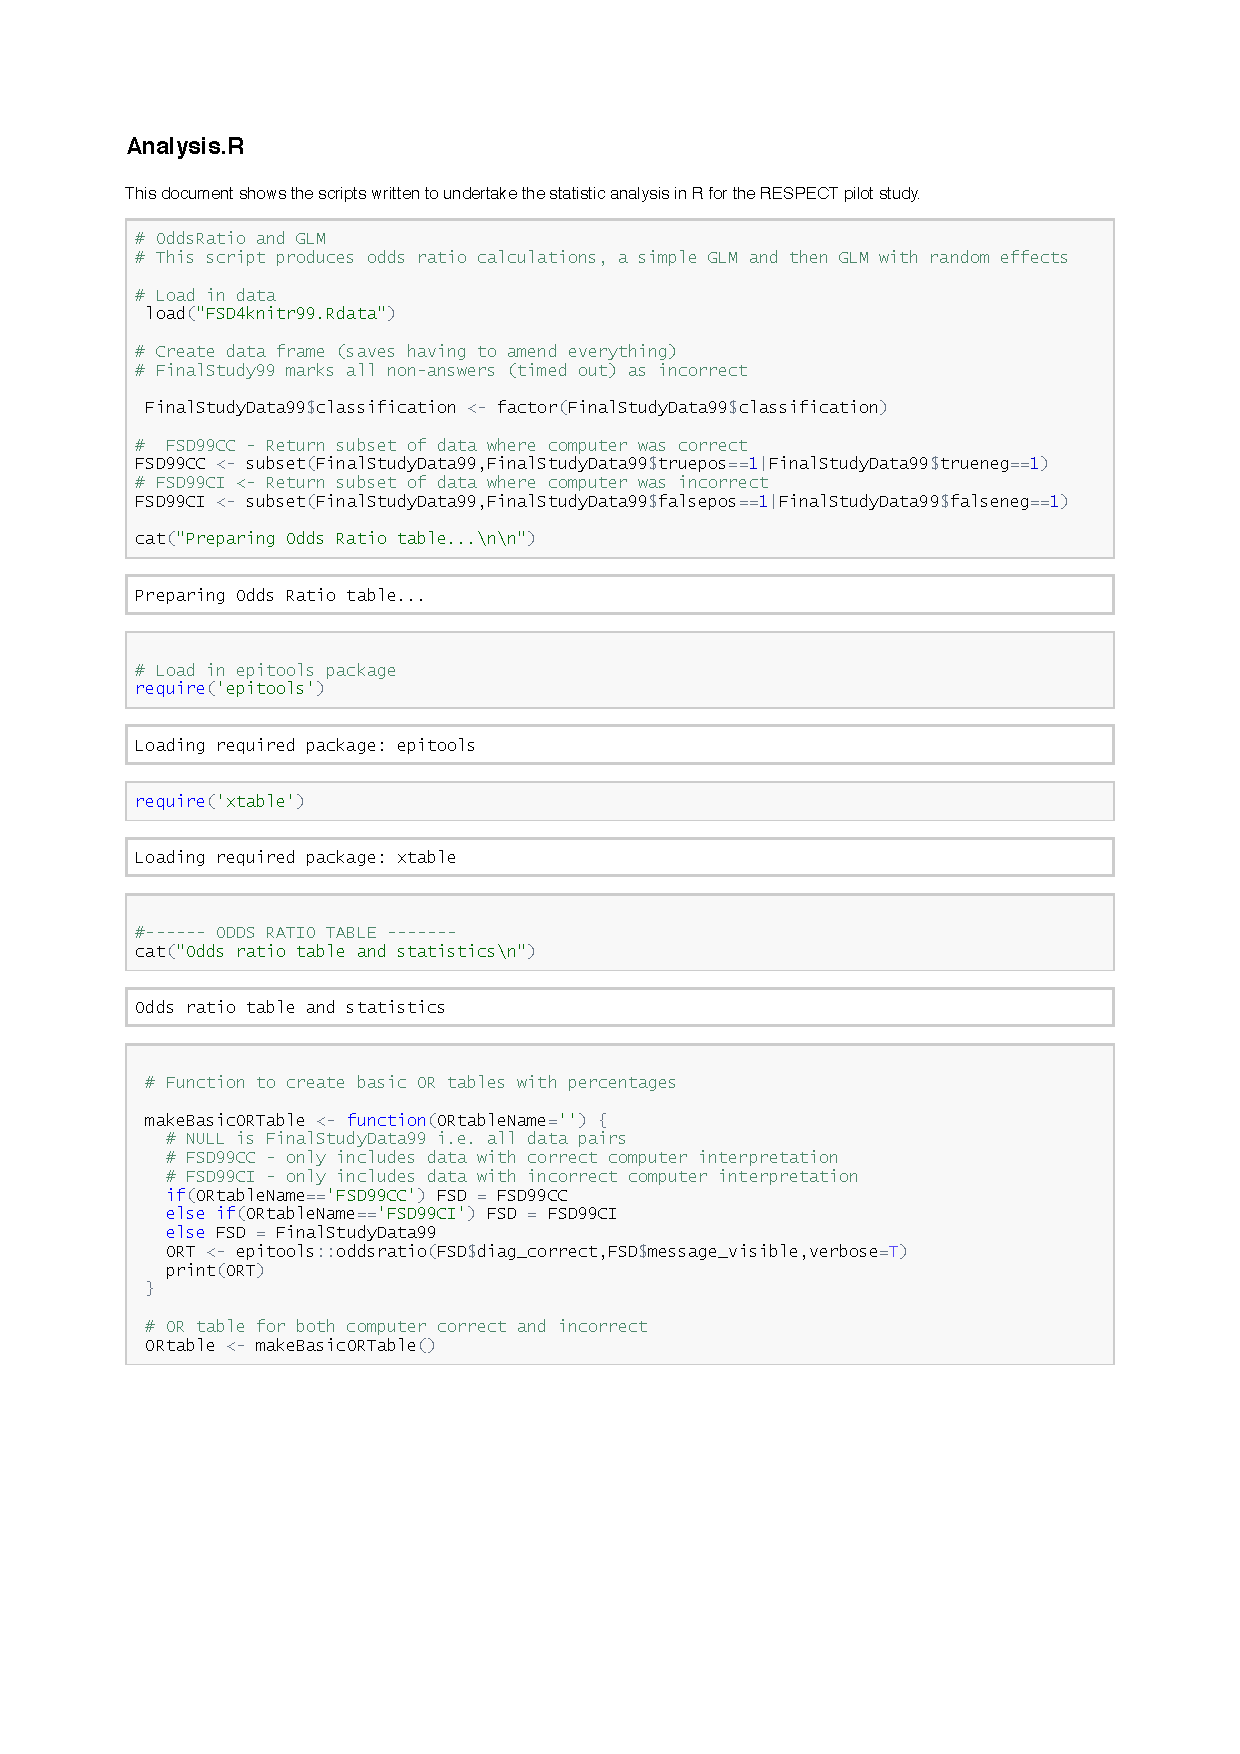
\includegraphics[page=1,keepaspectratio,width=0.80\paperwidth]{knitr.pdf}}
\end{figure}

\newpage

\begin{figure}[htbp]
\centerline{\includegraphics[page=2,keepaspectratio,width=0.80\paperwidth]{knitr.pdf}}
\end{figure}

\newpage

\begin{figure}[htbp]
\centerline{\includegraphics[page=3,keepaspectratio,width=0.80\paperwidth]{knitr.pdf}}
\end{figure}

\newpage

\begin{figure}[htbp]
\centerline{\includegraphics[page=4,keepaspectratio,width=0.80\paperwidth]{knitr.pdf}}
\end{figure}

\newpage

\begin{figure}[htbp]
\centerline{\includegraphics[page=5,keepaspectratio,width=0.80\paperwidth]{knitr.pdf}}
\end{figure}

\newpage

\begin{figure}[htbp]
\centerline{\includegraphics[page=6,keepaspectratio,width=0.80\paperwidth]{knitr.pdf}}
\end{figure}

\newpage

\begin{figure}[htbp]
\centerline{\includegraphics[page=7,keepaspectratio,width=0.80\paperwidth]{knitr.pdf}}
\end{figure}

\newpage

\begin{figure}[htbp]
\centerline{\includegraphics[page=8,keepaspectratio,width=0.80\paperwidth]{knitr.pdf}}
\end{figure}

\newpage

\begin{figure}[htbp]
\centerline{\includegraphics[page=9,keepaspectratio,width=0.80\paperwidth]{knitr.pdf}}
\end{figure}

\newpage

\begin{figure}[htbp]
\centerline{\includegraphics[page=10,keepaspectratio,width=0.80\paperwidth]{knitr.pdf}}
\end{figure}

\newpage

\begin{figure}[htbp]
\centerline{\includegraphics[page=11,keepaspectratio,width=0.80\paperwidth]{knitr.pdf}}
\end{figure}

\newpage

\begin{figure}[htbp]
\centerline{\includegraphics[page=12,keepaspectratio,width=0.80\paperwidth]{knitr.pdf}}
\end{figure}

\newpage

\begin{figure}[htbp]
\centerline{\includegraphics[page=13,keepaspectratio,width=0.80\paperwidth]{knitr.pdf}}
\end{figure}

\newpage

\begin{figure}[htbp]
\centerline{\includegraphics[page=14,keepaspectratio,width=0.80\paperwidth]{knitr.pdf}}
\end{figure}

\newpage

\begin{figure}[htbp]
\centerline{\includegraphics[page=15,keepaspectratio,width=0.80\paperwidth]{knitr.pdf}}
\end{figure}

\newpage

\begin{figure}[htbp]
\centerline{\includegraphics[page=16,keepaspectratio,width=0.80\paperwidth]{knitr.pdf}}
\end{figure}

\newpage

\begin{figure}[htbp]
\centerline{\includegraphics[page=17,keepaspectratio,width=0.80\paperwidth]{knitr.pdf}}
\end{figure}

\newpage

\begin{figure}[htbp]
\centerline{\includegraphics[page=18,keepaspectratio,width=0.80\paperwidth]{knitr.pdf}}
\end{figure}

\clearpage

\begin{figure}[htbp]
\centerline{\includegraphics[page=19,keepaspectratio,width=0.80\paperwidth]{knitr.pdf}}
\end{figure}

\newpage

\begin{figure}[htbp]
\centerline{\includegraphics[page=20,keepaspectratio,width=0.80\paperwidth]{knitr.pdf}}
\end{figure}

\newpage

\begin{figure}[htbp]
\centerline{\includegraphics[page=21,keepaspectratio,width=0.80\paperwidth]{knitr.pdf}}
\end{figure}

\newpage

\begin{figure}[htbp]
\centerline{\includegraphics[page=22,keepaspectratio,width=0.80\paperwidth]{knitr.pdf}}
\end{figure}

  % R stats output

% \input{./Appendices/AppendixK}  


\addtocontents{toc}{\vspace{2em}}  % Add a gap in the Contents, for aesthetics
\backmatter

%% ----------------------------------------------------------------

\label{References}
\lhead{\emph{References}}  % Change the left side page header to "Bibliography"
\bibliographystyle{vancouver}  % Use the "vancouver" BibTeX style for formatting the Bibliography
\bibliography{dissertation}  % The references (bibliography) information are stored in the file named "Bibliography.bib"

\end{document}  % The End
%% ----------------------------------------------------------------